\section{Discriminating variables}
\label{sec:ewk:sigbkg}

A key ingredient of the analysis is the reconstruction of the two Higgs bosons from the decay of the higgsinos.
Since this analysis targets events where both Higgs bosons decay to a $b\bar{b}$ pair, the reconstruction starts 
from four jets, which are chosen according to an ordering that favors $b$-tagged jets over non-tagged jets,
and then orders based on \pt. Practically, this results in the following criteria:
\begin{itemize}
\item If there are exactly four $b$-tagged jets in the event, those are used.
\item If there are more than four $b$-tagged jets, the selected ones are the four $b$-tagged jets with highest \pt.
\item If there are less than four $b$-tagged jets, the selected ones are the $b$-tagged jets and the non-tagged jets with highest \pt.
\end{itemize} 

Once the four jets have been selected, they are grouped in two pairs, each one constituting a candidate Higgs bosons. 
Different algorithms to pair the jets have been tested, and the chosen one is based on minimizing the angular separation 
between the two jets associated to the same Higgs boson candidate. 
In particular, the permutation chosen is the one that minimizes:
\begin{equation}
\dRmax = \mathrm{max}(\Delta R(h_1), \Delta R(h_2)) \; ,
\end{equation}

\noindent where $\Delta R(h)$ is the distance in the $\eta-\phi$ space between the two jets from the same candidate.
This choice has a good efficiency in reconstructing the Higgs bosons in the signal, 
and at the same time avoids creating artificial peaks in the background in correspondence of the Higgs boson mass. 
More details on the efficiency of the reconstruction and the comparison with other reconstruction algorithms are given in 
Appendix \ref{app:higgs}.

Beside the variables described in Section \ref{sec:common_variables}, a few other discriminating variables particularly 
effective for this signal model are described below.

\subsubsection*{Candidate Higgs bosons}

The invariant mass of the two Higgs boson candidates built following the procedure outlined above 
are used as discriminating variable. In particular, we refer to m($h_1$) and m($h_2$) respectively for the mass of the Higgs candidate with 
the leading and subleading mass.

The variable \dRmax, defined in the previous section, is used to choose the pairing of the jets while reconstructing 
the Higgs boson candidates but also as a discriminating variable to separate signal and background. 

\subsubsection*{Modified effective mass}

In the signal model, only four jets come from the hard scattering process, and are therefore expected to be more energetic than the 
remaining jets in the event. Therefore the \meff definition is modified to include only the jets that are selected 
as originating from a Higgs boson; the modified definition is therefore:
\begin{equation}
\meffb = \sum_{i=1,..,4} {\pt}^{j_i} + \met
\end{equation}
\noindent where the sum runs over the jets selected according to the ordering procedure presented in Section \ref{sec:ewk:higgsreco}. 


The variables defined above, together with the ones defined in Section \ref{sec:common_variables} 
allow identifying a region of the phase space that is enriched in signal events. 
This study is performed after selecting events with high \met ($> 200$ GeV), at least four signal jets and, least three $b$-tagged jets, zero signal leptons and \dphimin $>0.4$.

Figures \ref{fig:ewk:sig:1} and \ref{fig:ewk:sig:2}  show the distribution of the main kinematic variables for 
the sum of the \gls{sm} backgrounds and for different signal samples after these selections.
Figures \ref{fig:ewk:sig:mass_h1_min_dR} and \ref{fig:ewk:sig:mass_h2_min_dR} show the distribution of the mass of the Higgs 
candidate with the leading and subleading mass respectively. As can be appreciated, the distribution peaks at values around the Higgs mass for 
signals, while it is flatter for background. 
The distribution of \dRmax is shown in Figure \ref{fig:ewk:sig:dRmax_dR}. This variable assumes in general a lower value for 
signal events, in particular for the high-mass signals, where the Higgs bosons are produced with higher \pt and thus have 
more collimated decay products. Signal events also tend to have a lower number of signal jets, as can be observed in Figure 
\ref{fig:ewk:sig:jets_n}, and they occupy mostly the bins with three and four $b$-jets in the 
distribution of \nbjet (Figure \ref{fig:ewk:sig:bjets_n}). 
The \met distribution, shown in Figure \ref{fig:ewk:sig:met}, displays the expected features: while signals with low-mass higgsinos 
have low \met values, the distribution tends to assume increasingly high values with the increase of the higgsino mass. 
A similar feature is shown in Figures \ref{fig:ewk:sig:meff_4bj} and \ref{fig:ewk:sig:mTb_min} for the \meffb and \mtb distributions respectively: 
the higher the higgsino mass in the signal, the more signal events differ from background events. 
While on the one hand this makes it easier to separate them from the \gls{sm} background, on the other hand the increase in signal mass 
implies a decrease in production cross-section, which will be the limiting factor in sensitivity to high-mass signals. 

\begin{figure*}[htbp]
\centering 
\subfigure[m($h_1$)]{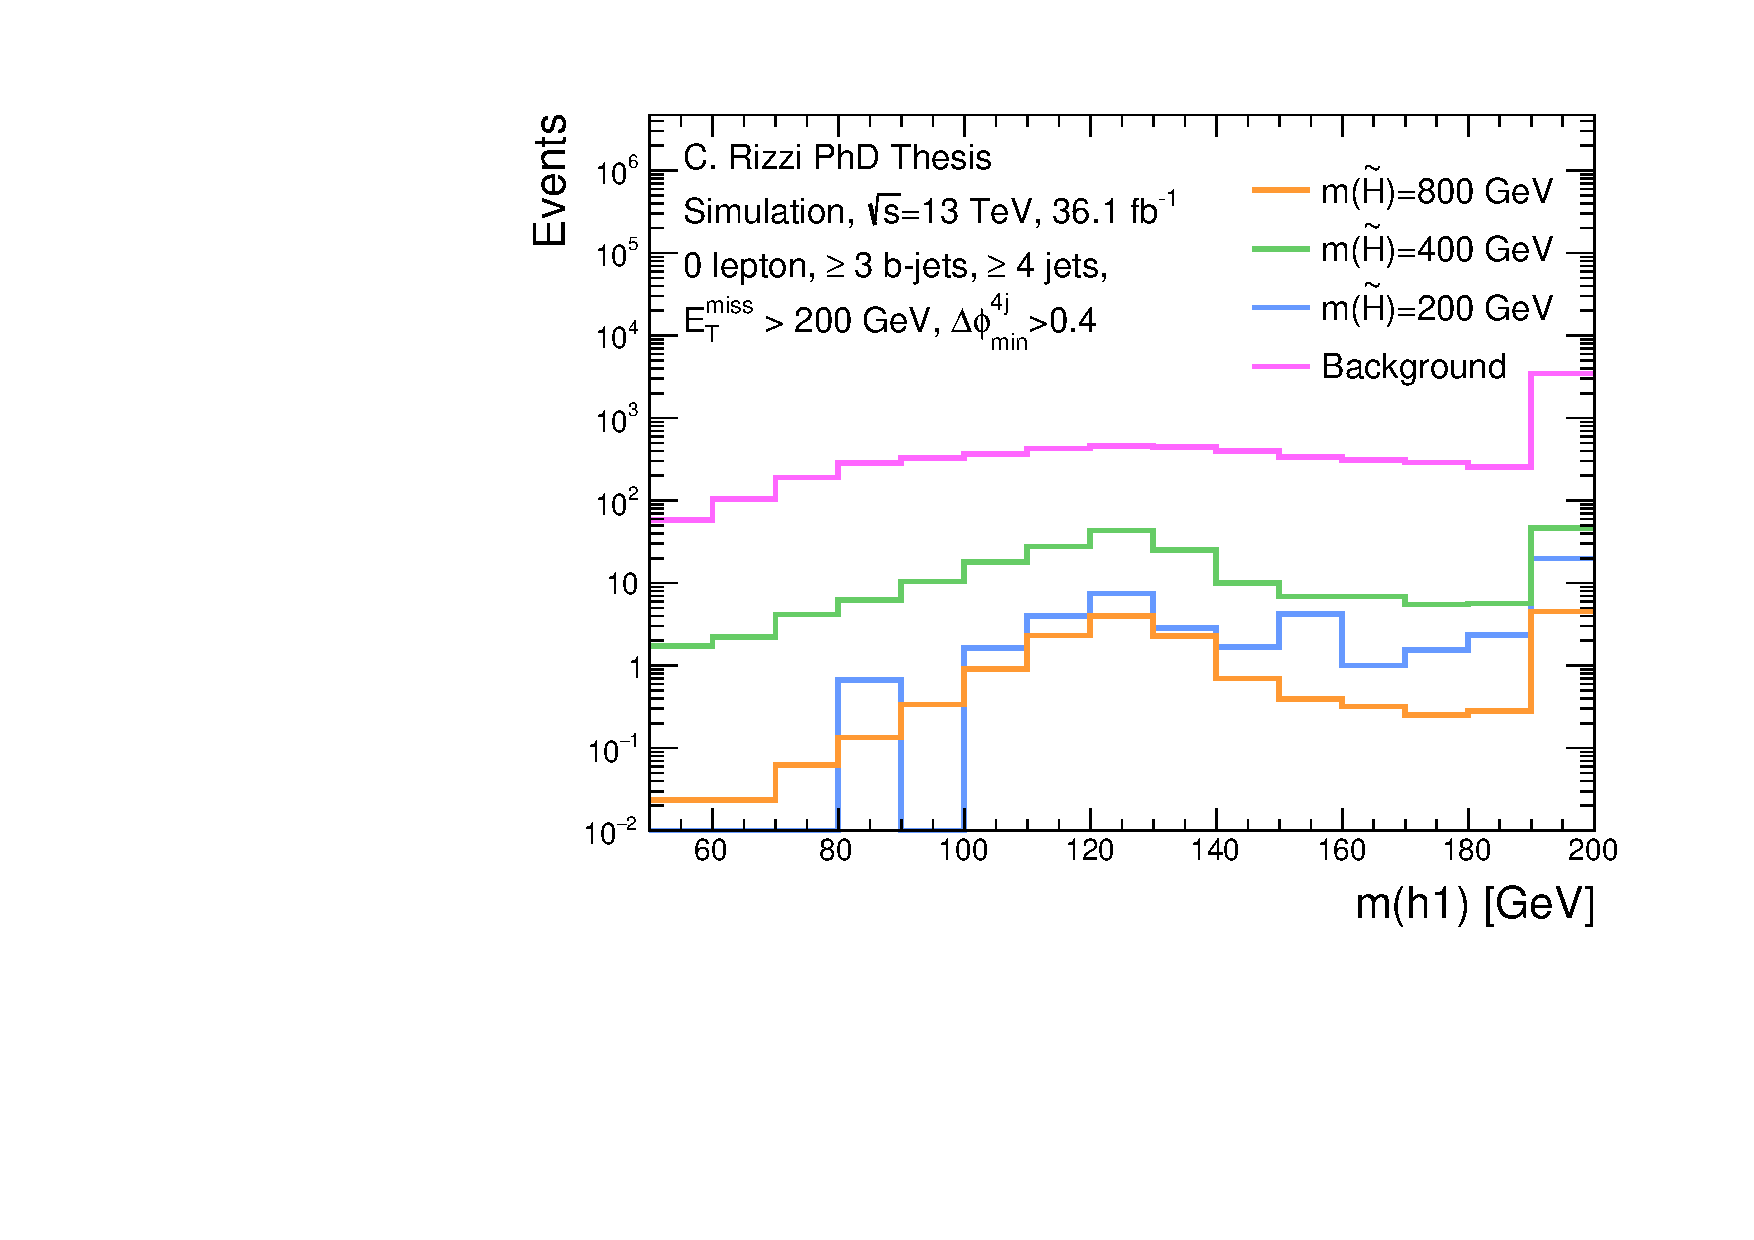
\includegraphics[width=0.48\textwidth]{figures/ewk_prod/sig_bkg/hh_compare_mass_h1_min_dR.pdf}\label{fig:ewk:sig:mass_h1_min_dR}}
\subfigure[m($h_2$)]{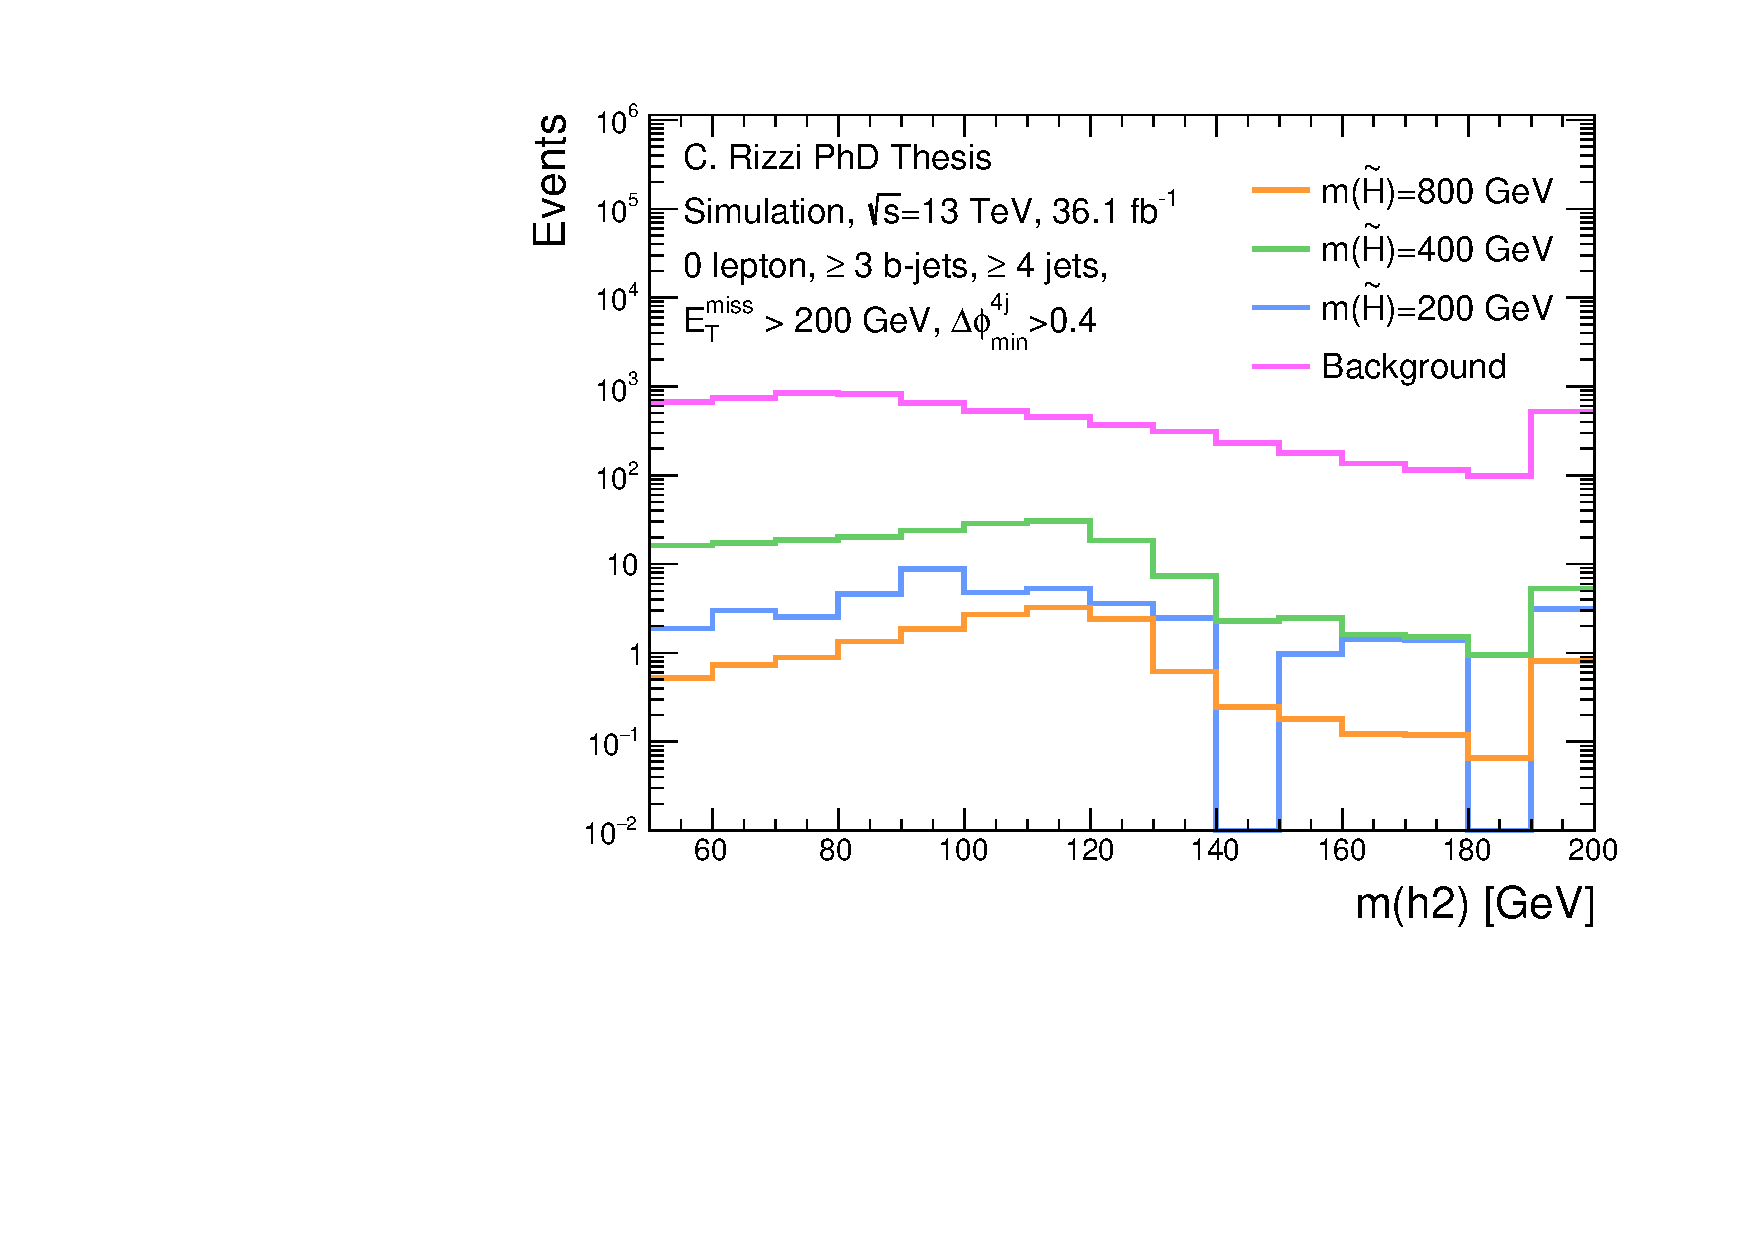
\includegraphics[width=0.48\textwidth]{figures/ewk_prod/sig_bkg/hh_compare_mass_h2_min_dR.pdf}\label{fig:ewk:sig:mass_h2_min_dR}} \\
\subfigure[\dRmax]{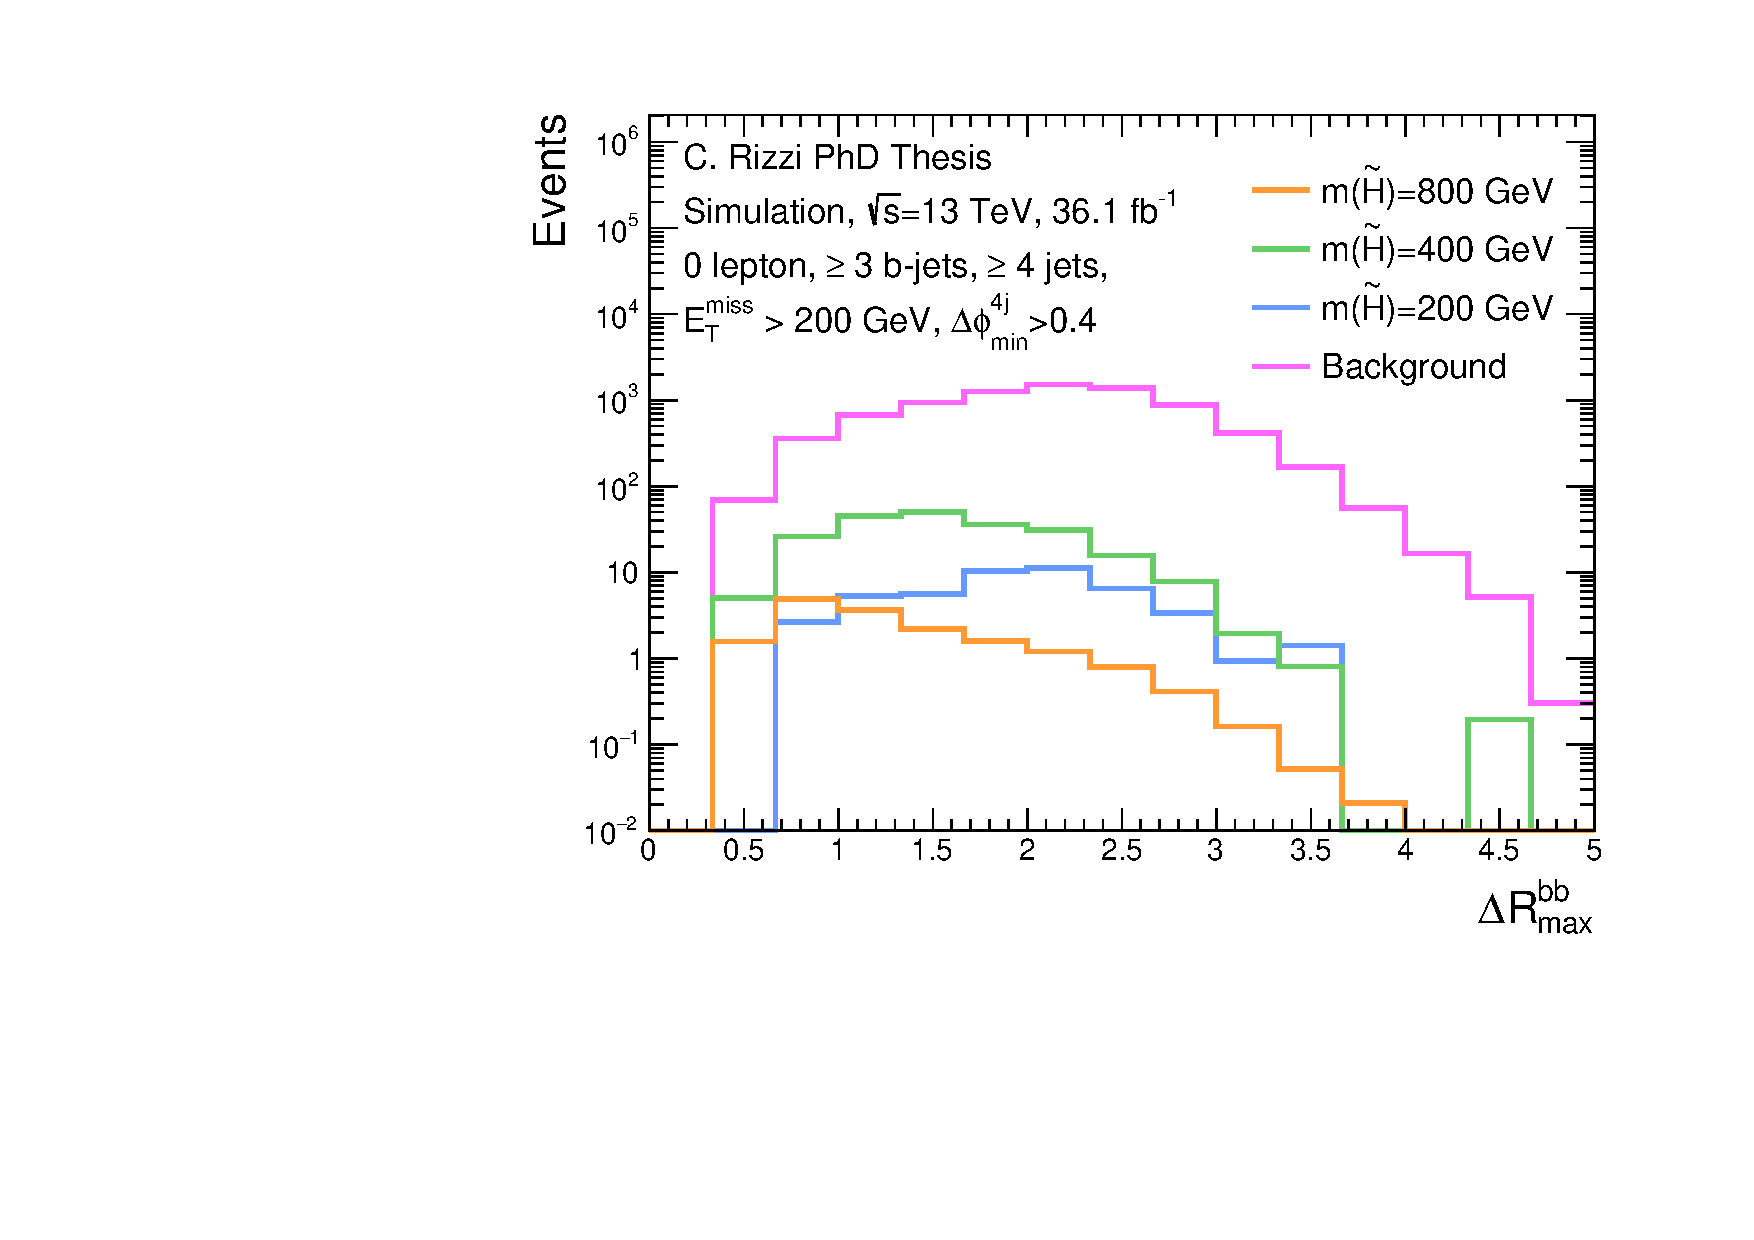
\includegraphics[width=0.48\textwidth]{figures/ewk_prod/sig_bkg/hh_compare_dRmax_dR.pdf}\label{fig:ewk:sig:dRmax_dR}}
\subfigure[\meffb]{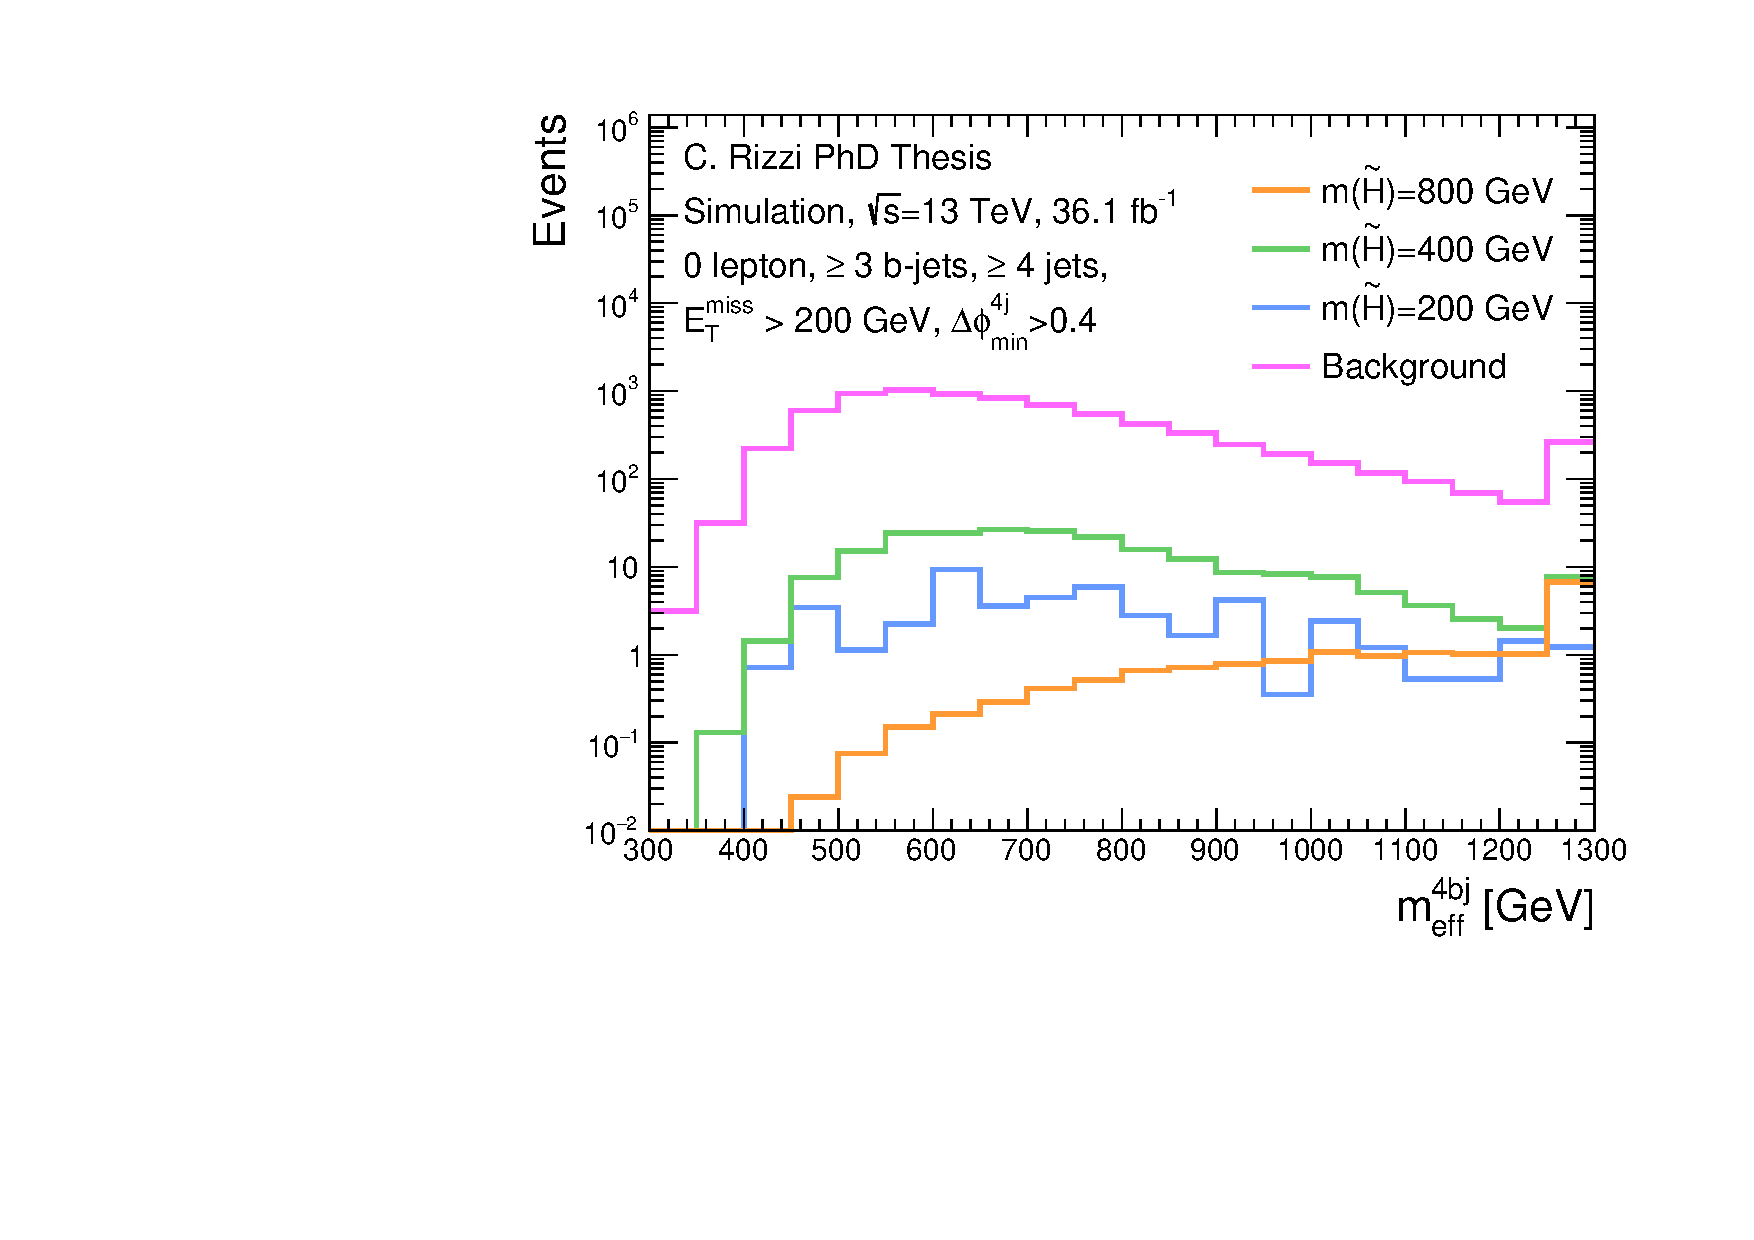
\includegraphics[width=0.48\textwidth]{figures/ewk_prod/sig_bkg/hh_compare_meff_4bj.pdf}\label{fig:ewk:sig:meff_4bj}}
\caption{Distribution of  the main kinematic variables in background and signal events after the selections described in the text.}
\label{fig:ewk:sig:1}
\end{figure*}

\begin{figure*}[htbp]
\centering
\subfigure[\njet]{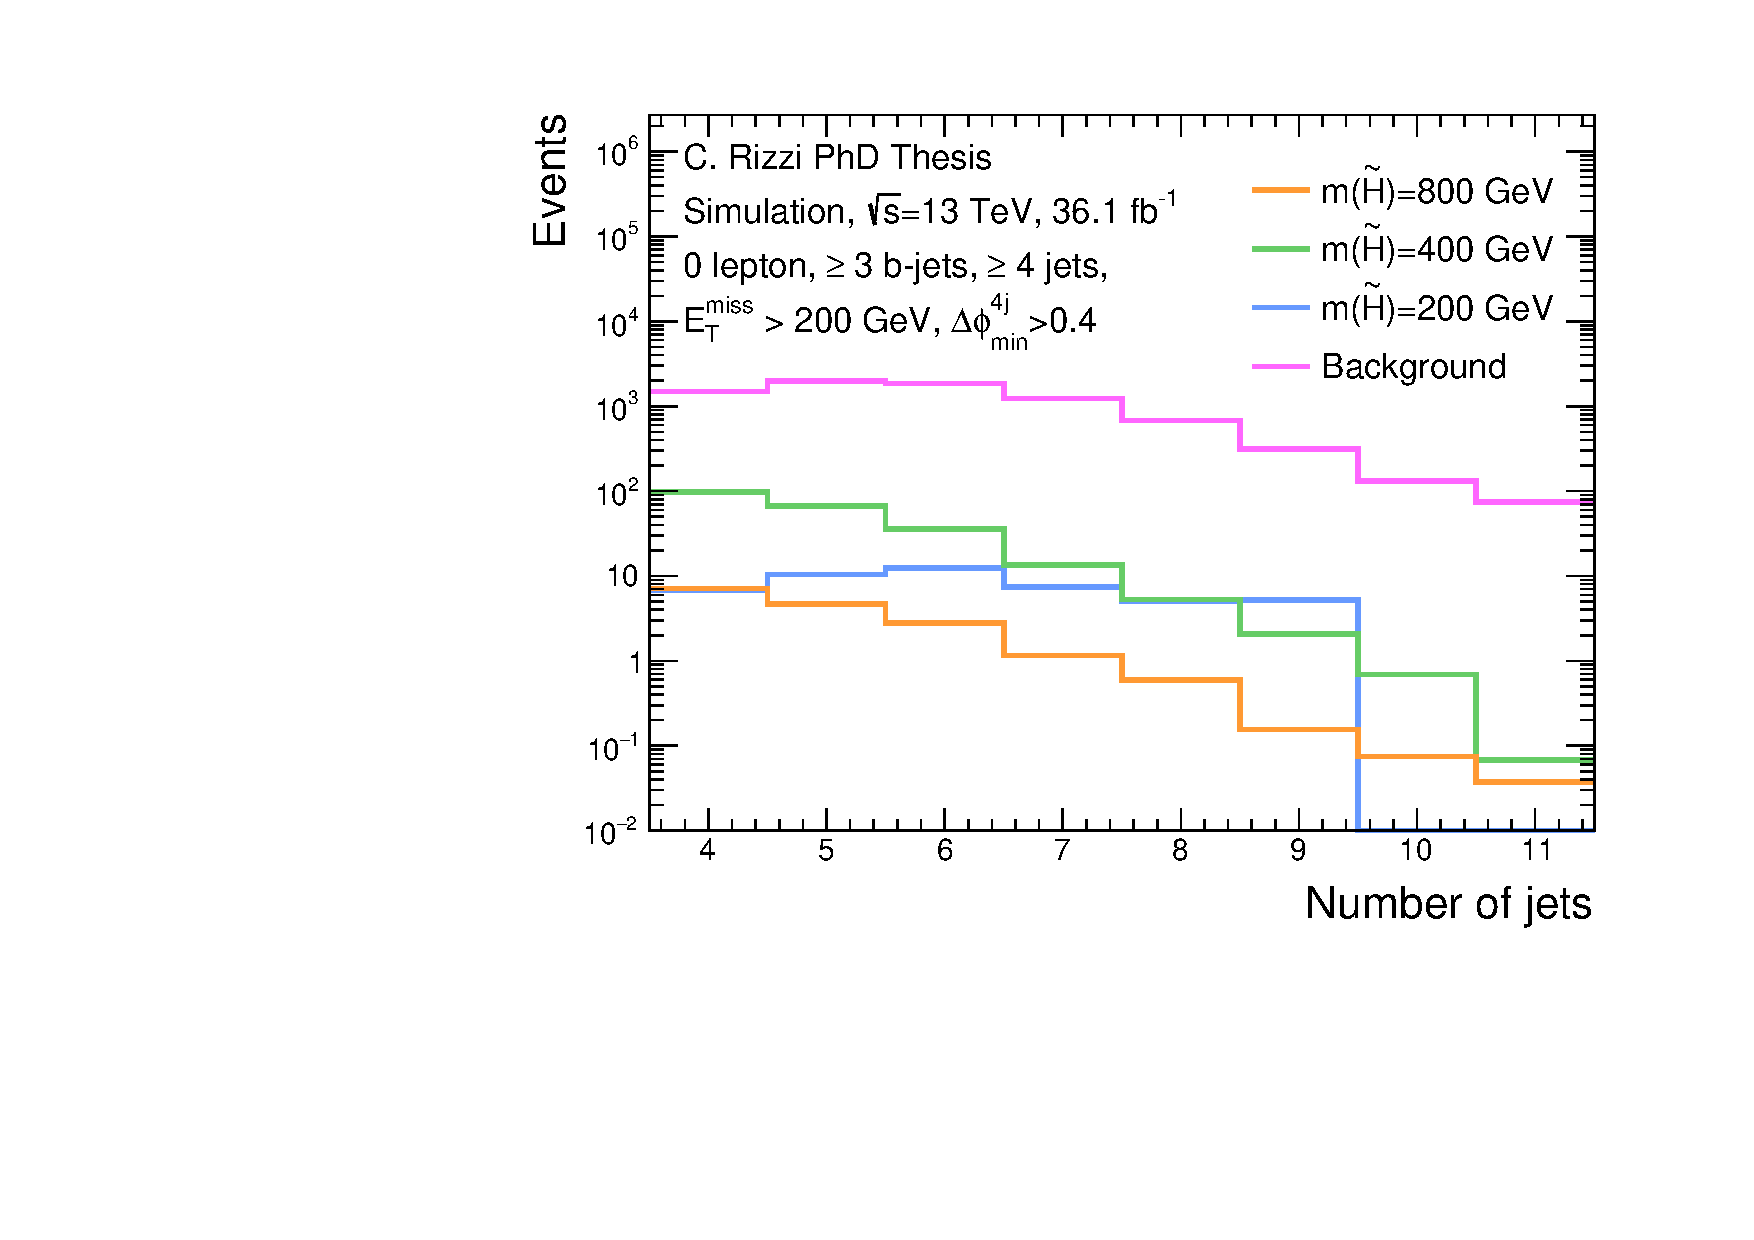
\includegraphics[width=0.48\textwidth]{figures/ewk_prod/sig_bkg/hh_compare_jets_n.pdf}\label{fig:ewk:sig:jets_n}}
\subfigure[\nbjet]{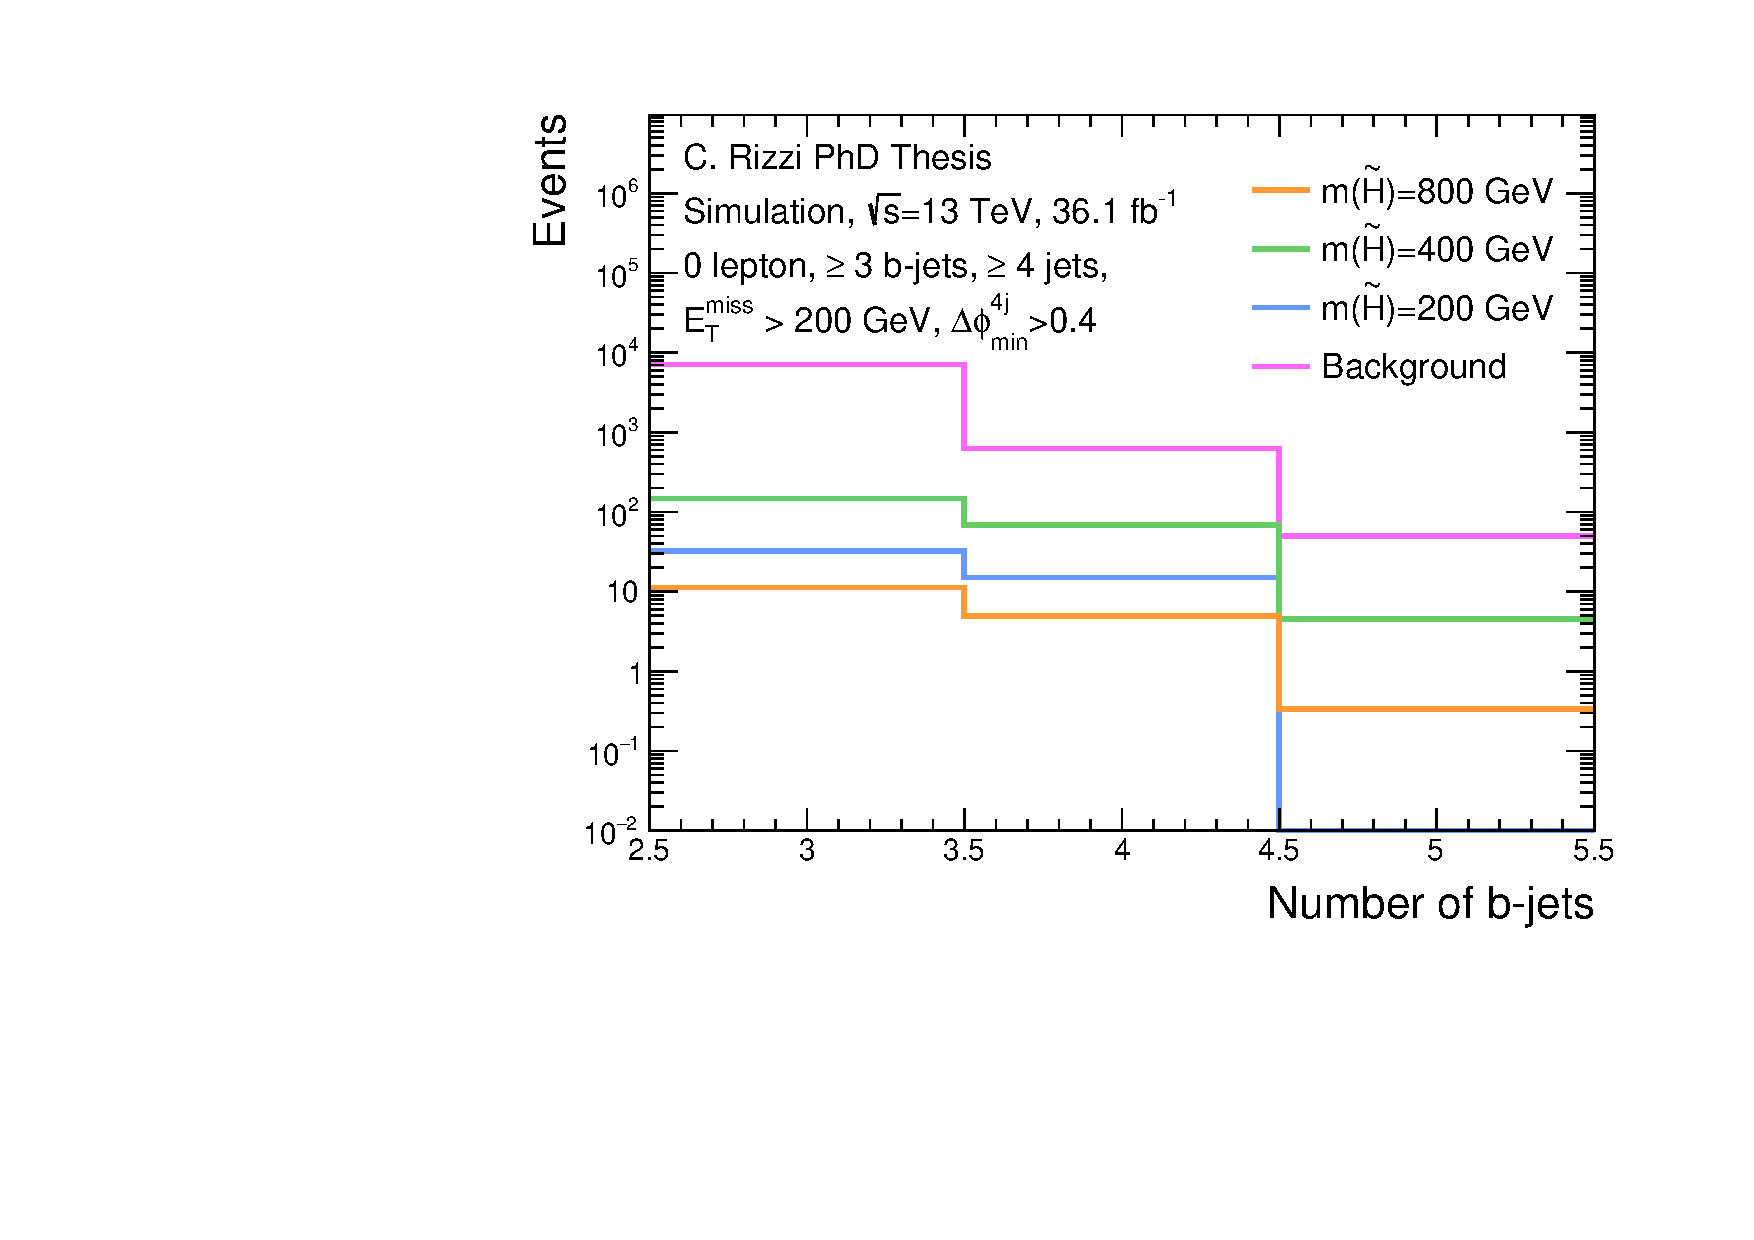
\includegraphics[width=0.48\textwidth]{figures/ewk_prod/sig_bkg/hh_compare_bjets_n.pdf}\label{fig:ewk:sig:bjets_n}}\\
\subfigure[\met]{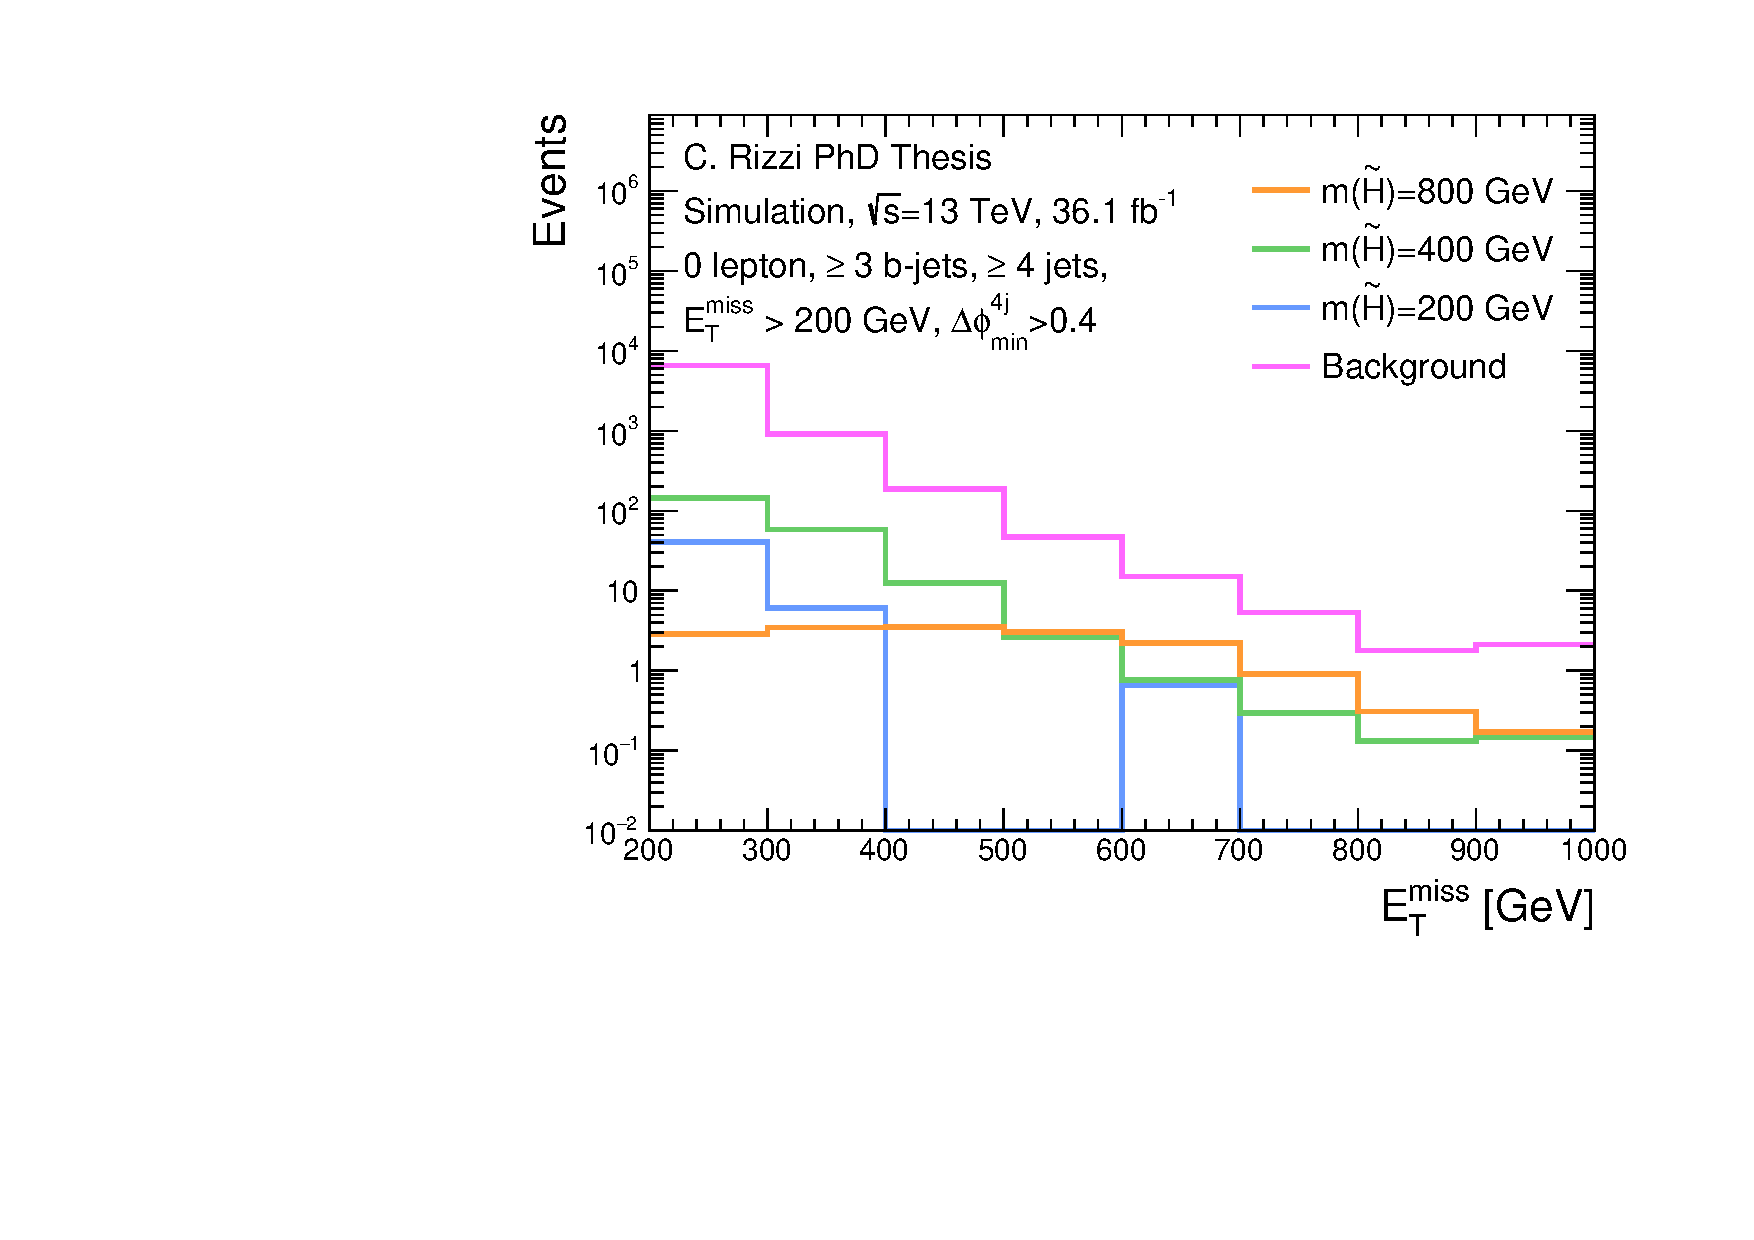
\includegraphics[width=0.48\textwidth]{figures/ewk_prod/sig_bkg/hh_compare_met.pdf}\label{fig:ewk:sig:met}}
\subfigure[\mtb]{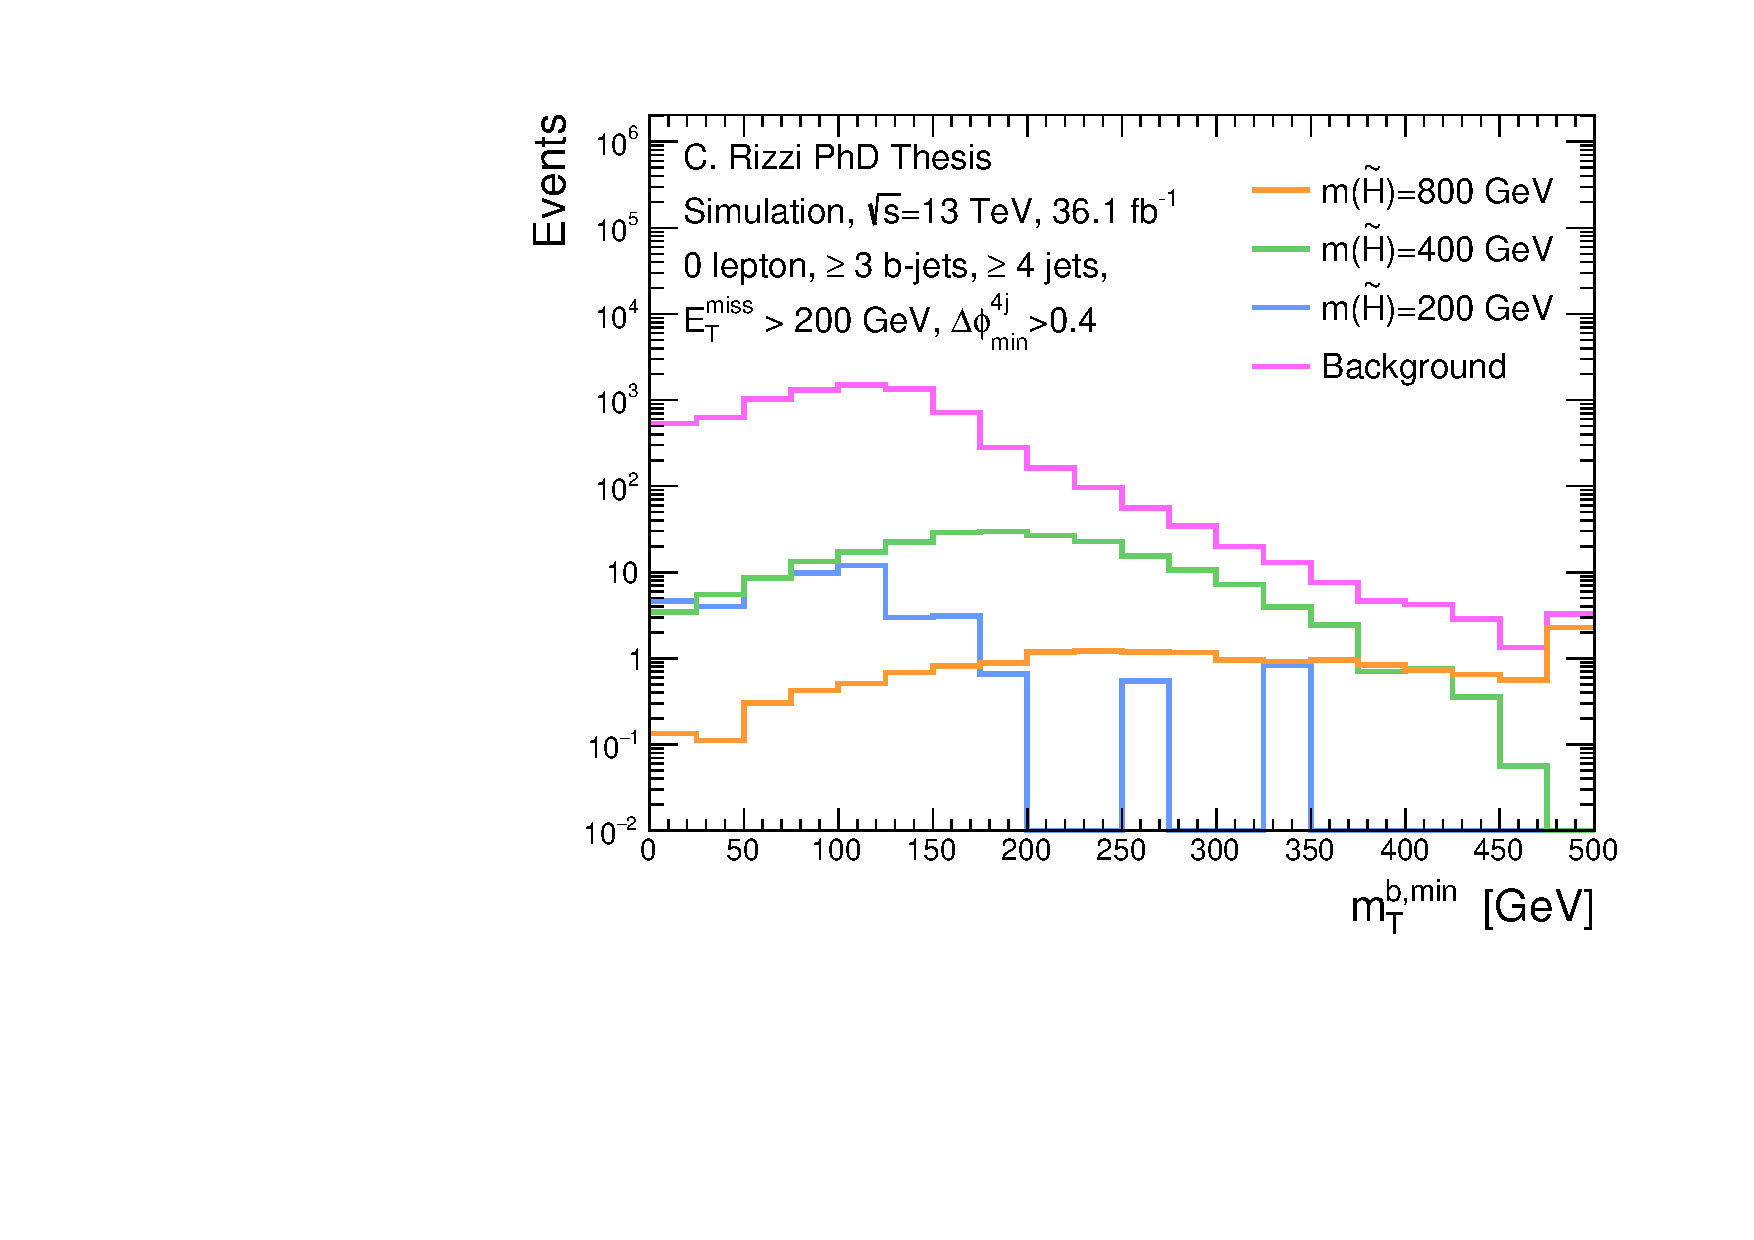
\includegraphics[width=0.48\textwidth]{figures/ewk_prod/sig_bkg/hh_compare_mTb_min.pdf}\label{fig:ewk:sig:mTb_min}}
\caption{Distribution of  the main kinematic variables in background and signal events after the selections described in the text.}
\label{fig:ewk:sig:2}
\end{figure*}

\FloatBarrier

\section{Signal regions}
\label{sec:ewk:SR}

This section describes the optimization of the \glspl{sr}. 
The high branching ratio of the h$\rightarrow$bb (58\%) makes the $\geq$3b channel the most promising to look for signal models 
in which both $\ninoone$ decay to h+$\gravino$. 
Therefore, the analysis selection are optimized to maximize the expected sensitivity to signals leading to $hh+\met$ 
and all the \glspl{sr} require both boson candidates to have masses compatible with the Higgs mass (the specific mass range is chosen during the optimization). 
%The target signal model is shown in Figure \ref{fig:opt_sighh4b}.

\subsection{Multi-bin regions}
\label{sec:ewk:multibin}

The optimization of the multi-bin \glspl{sr} aims at constructing several orthogonal \glspl{sr}, that can be combined in a fit. 
The general strategy adopted follows these steps:
\begin{enumerate}
\item A first variable (var$_1$) is chosen to define a coarse binning. 
    This variable should provide both a good signal-to-background discrimination and discrimination between signal 
    with different higgsino masses.
\item For each of these bins in var$_1$, a \gls{cr} is defined to normalize the \ttbar background in a kinematic regime close to the corresponding \gls{sr}.
\item Each bin based on var$_1$ is further split based on a second variable, var$_2$ (in this case all the bins based on the second variable share the same \gls{cr}).
\item The selections on the remaining kinematic variables are optimized independently in each var$_1$ bin (i.e. all the regions sharing the same 
\gls{cr} have the same selections on all the variables except var$_2$).
\end{enumerate}

\noindent As described above, var$_1$ must be able to provide at the same time a good separation between signal and background 
and a good separation between signals with different \hino masses. 
The latter is necessary in order to be able to optimize each bin in var$_1$ based on a different signal mass, 
providing in the end a good sensitivity to the entire mass spectrum. 
In order to understand which variable works best for this scope, the separation algorithm provided by the TMVA toolkit \footnote{TMVA is a toolkit designed for multivariate analyses, this in not the case here: it's only used as a quick way to access the discrimination power of the individual variables.} \cite{Hocker:2007ht} is used, defined as:

\begin{equation}
          \mathrm{separation} = \frac{1}{2} \int\frac{\left(f_s(x) - f_b(x)\right)^2}{f_s(x) + f_b(x)} dx \; , 
\label{eq:separation}
\end{equation}
\noindent where $f_s$ and $f_b$ are the signal and background \glspl{pdf} of $x$. 

The separation provided by the most promising analysis variables between background and 
signals with m(\hino)=300, 500 and 800 GeV is shown in Figure \ref{fig:ewk:separation}.
It is possible to see that \meffb is the best variable for our requirements (even if there are individual bins where this is not the case). 

\begin{figure}[htpb]
\begin{center}
%\subfigure[]{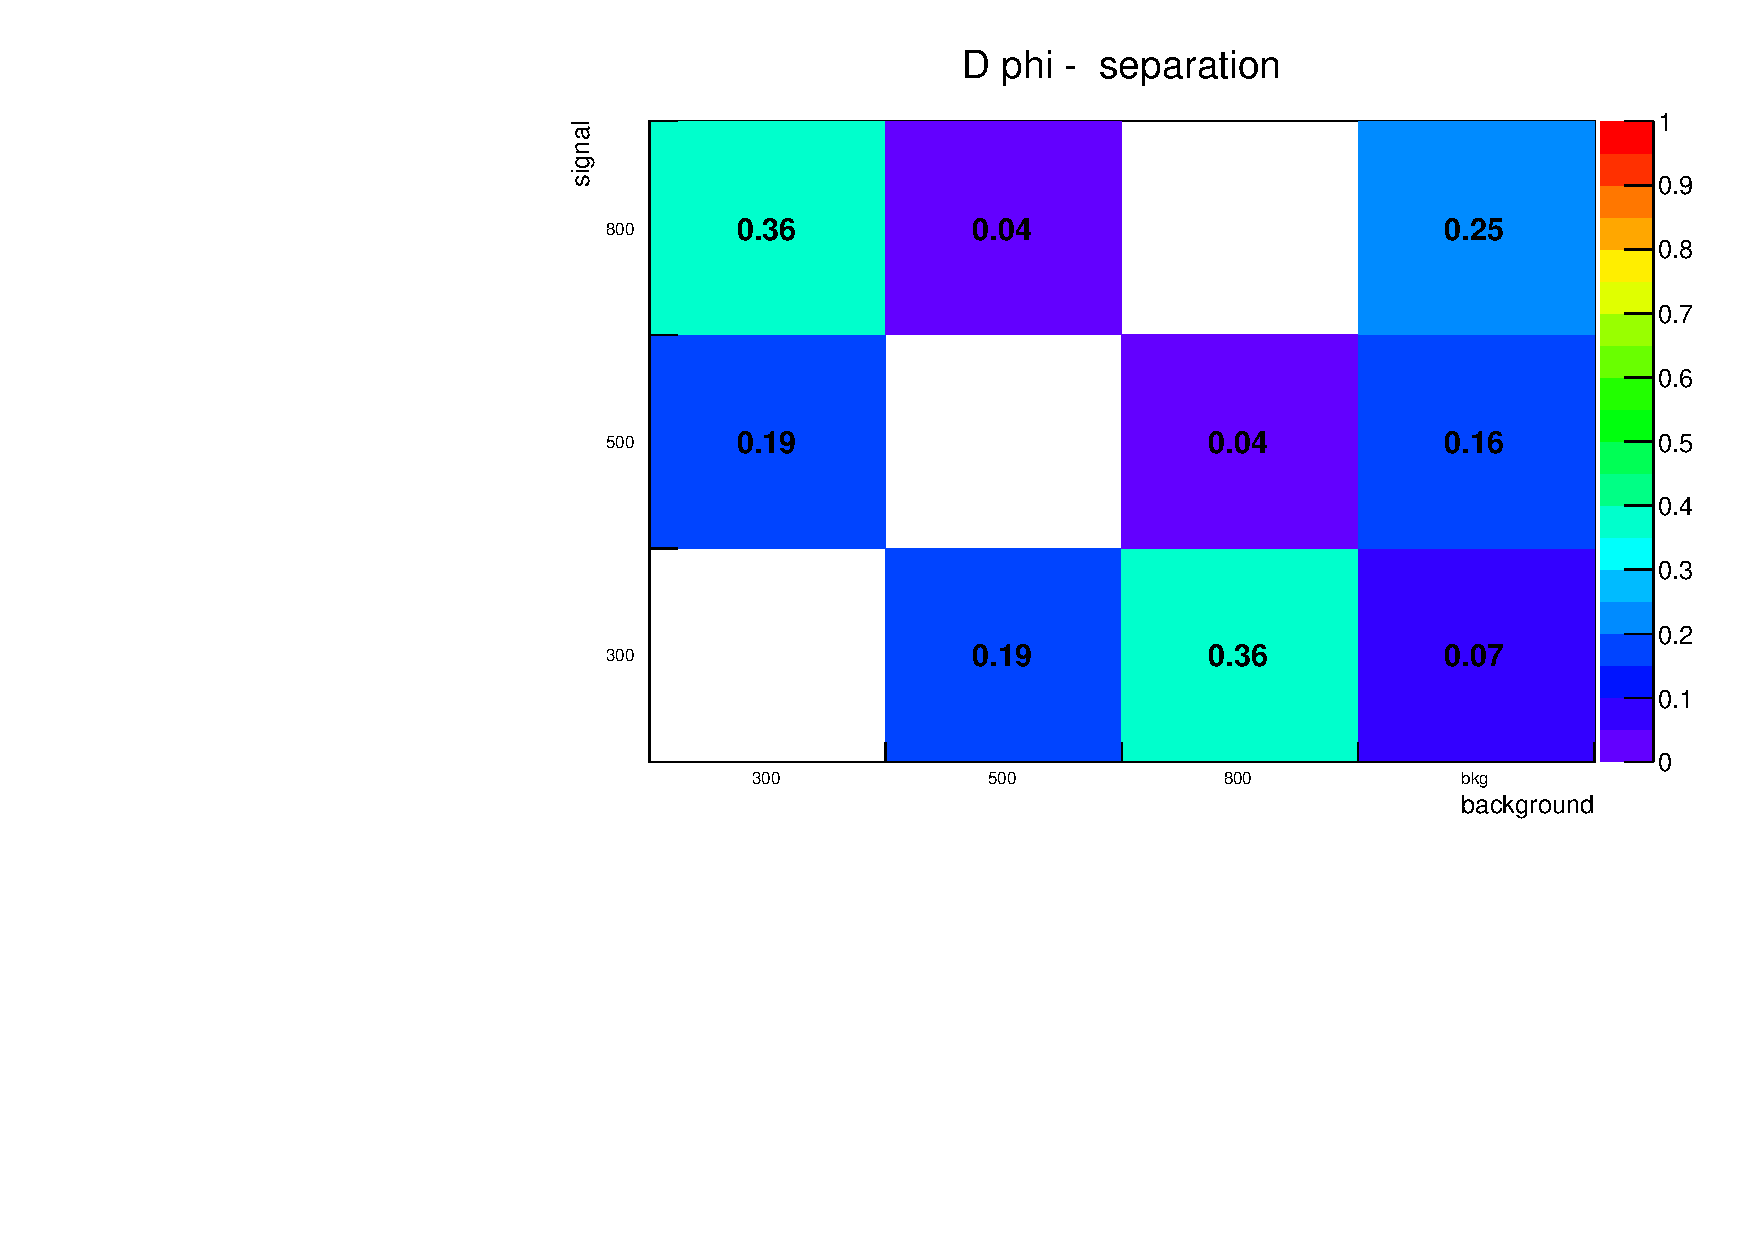
\includegraphics[width=0.43\textwidth]{figures/ewk_prod/separation/saparation_Dphi.pdf}}
\subfigure[]{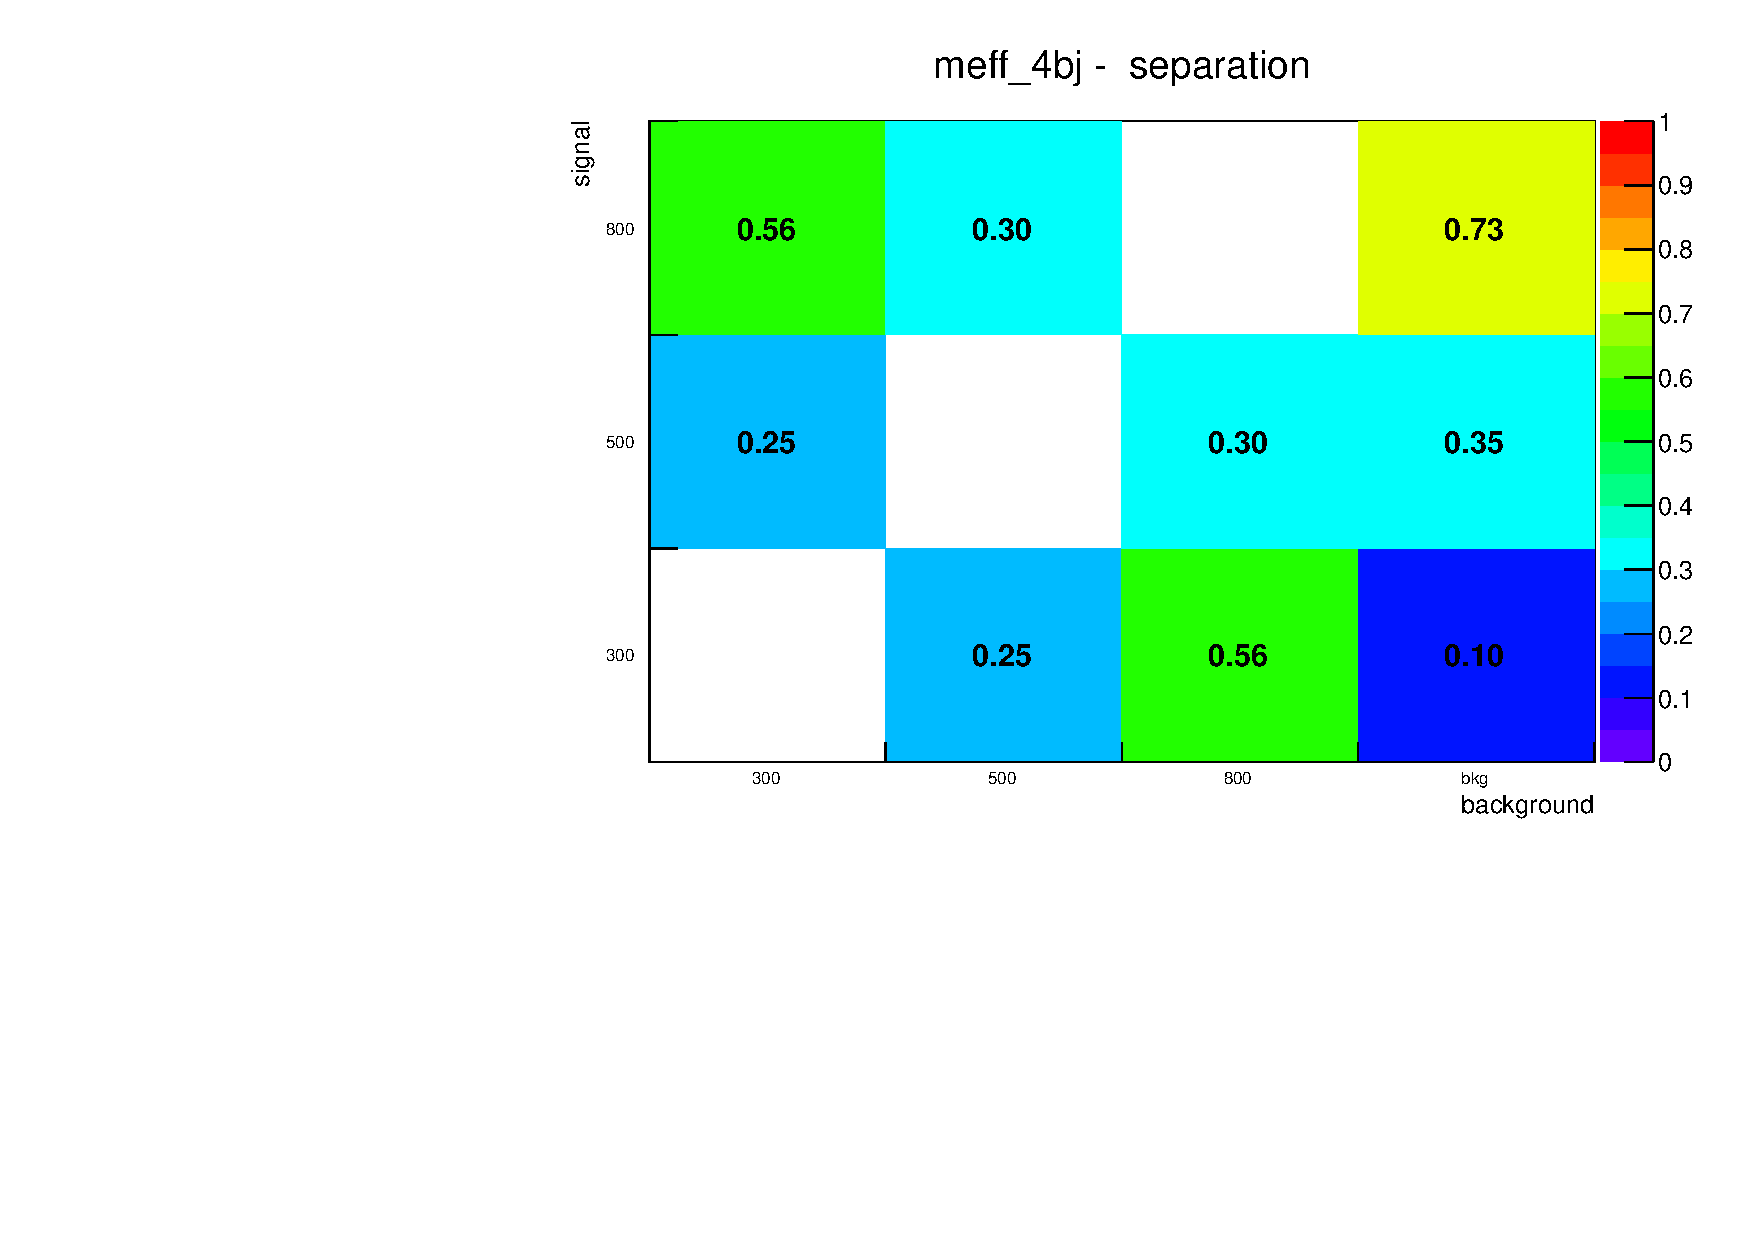
\includegraphics[width=0.43\textwidth]{figures/ewk_prod/separation/saparation_meff_4bj.pdf}}
\subfigure[]{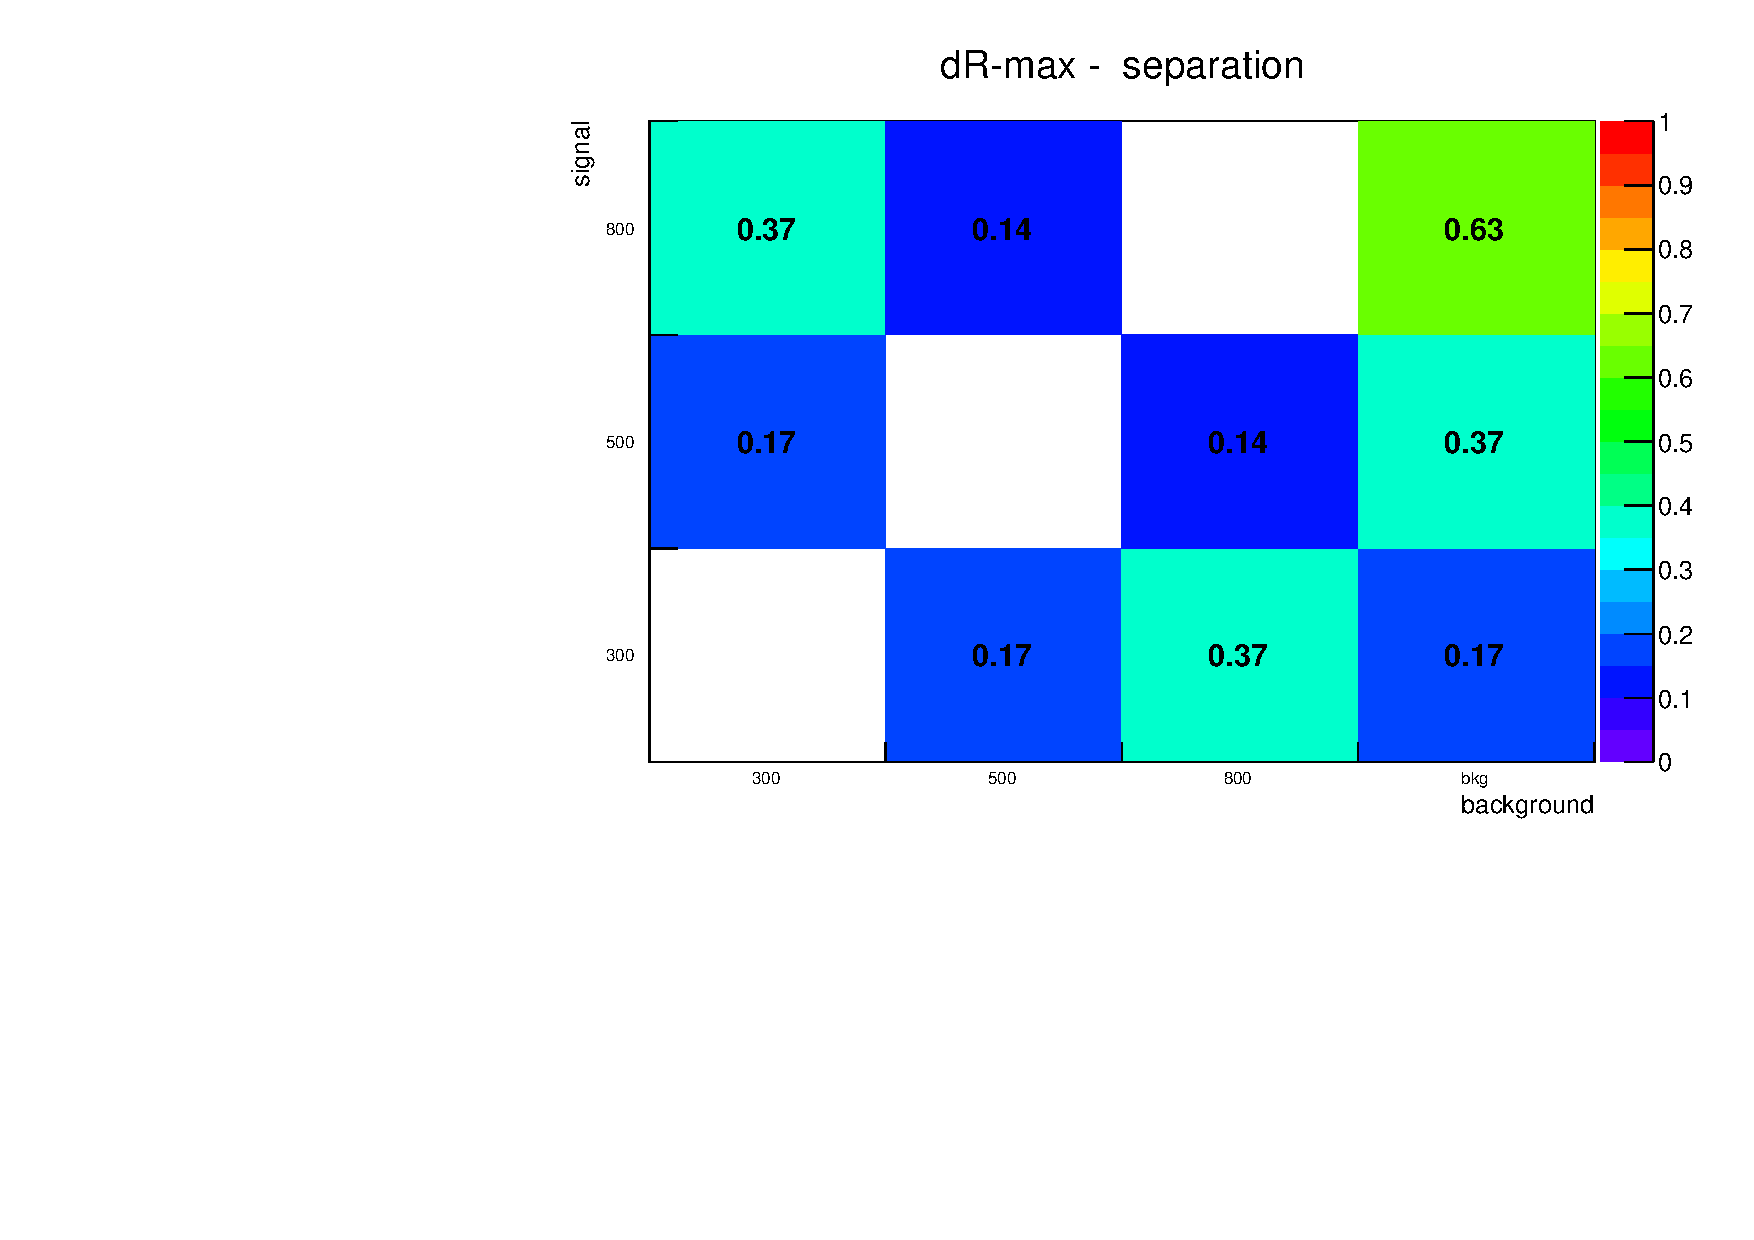
\includegraphics[width=0.43\textwidth]{figures/ewk_prod/separation/saparation_dR_max.pdf}}\\
\subfigure[]{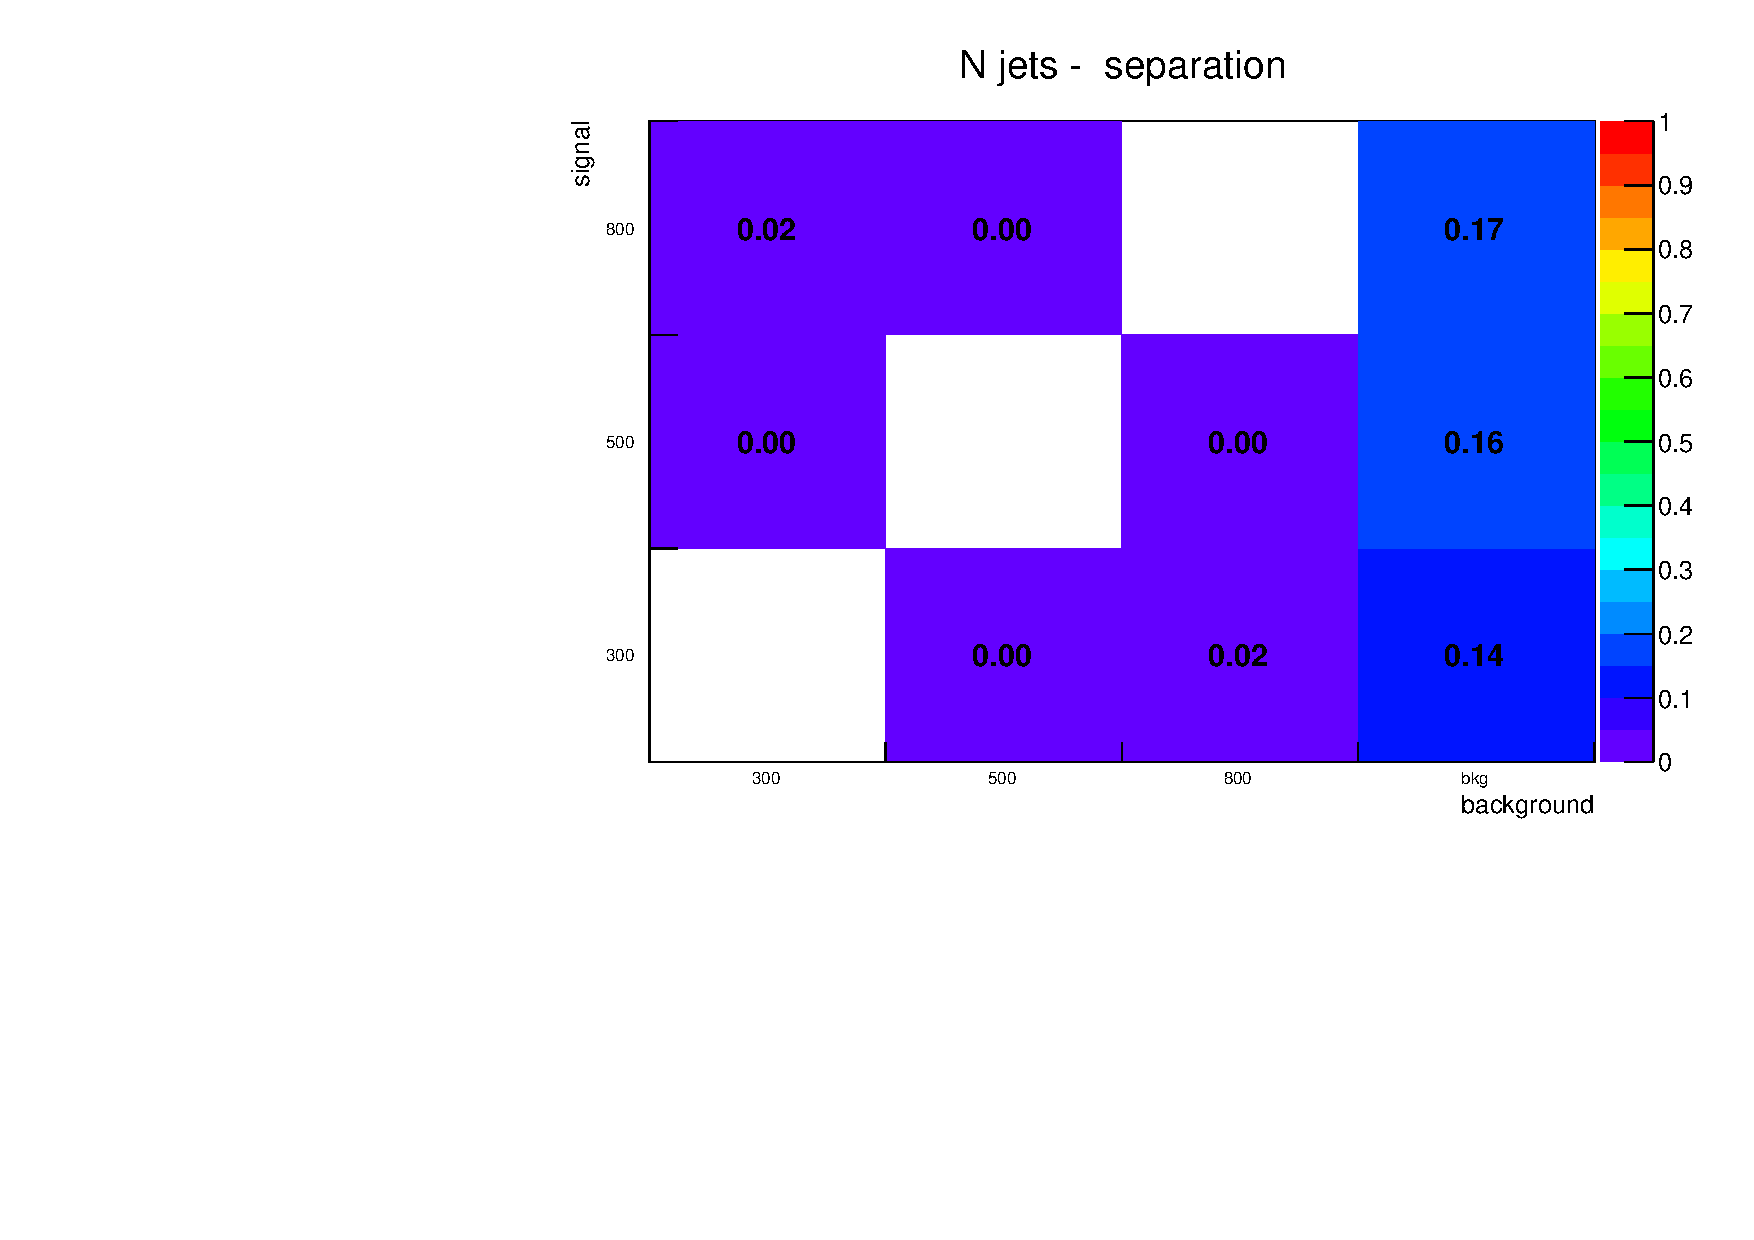
\includegraphics[width=0.43\textwidth]{figures/ewk_prod/separation/saparation_Njets.pdf}}
\subfigure[]{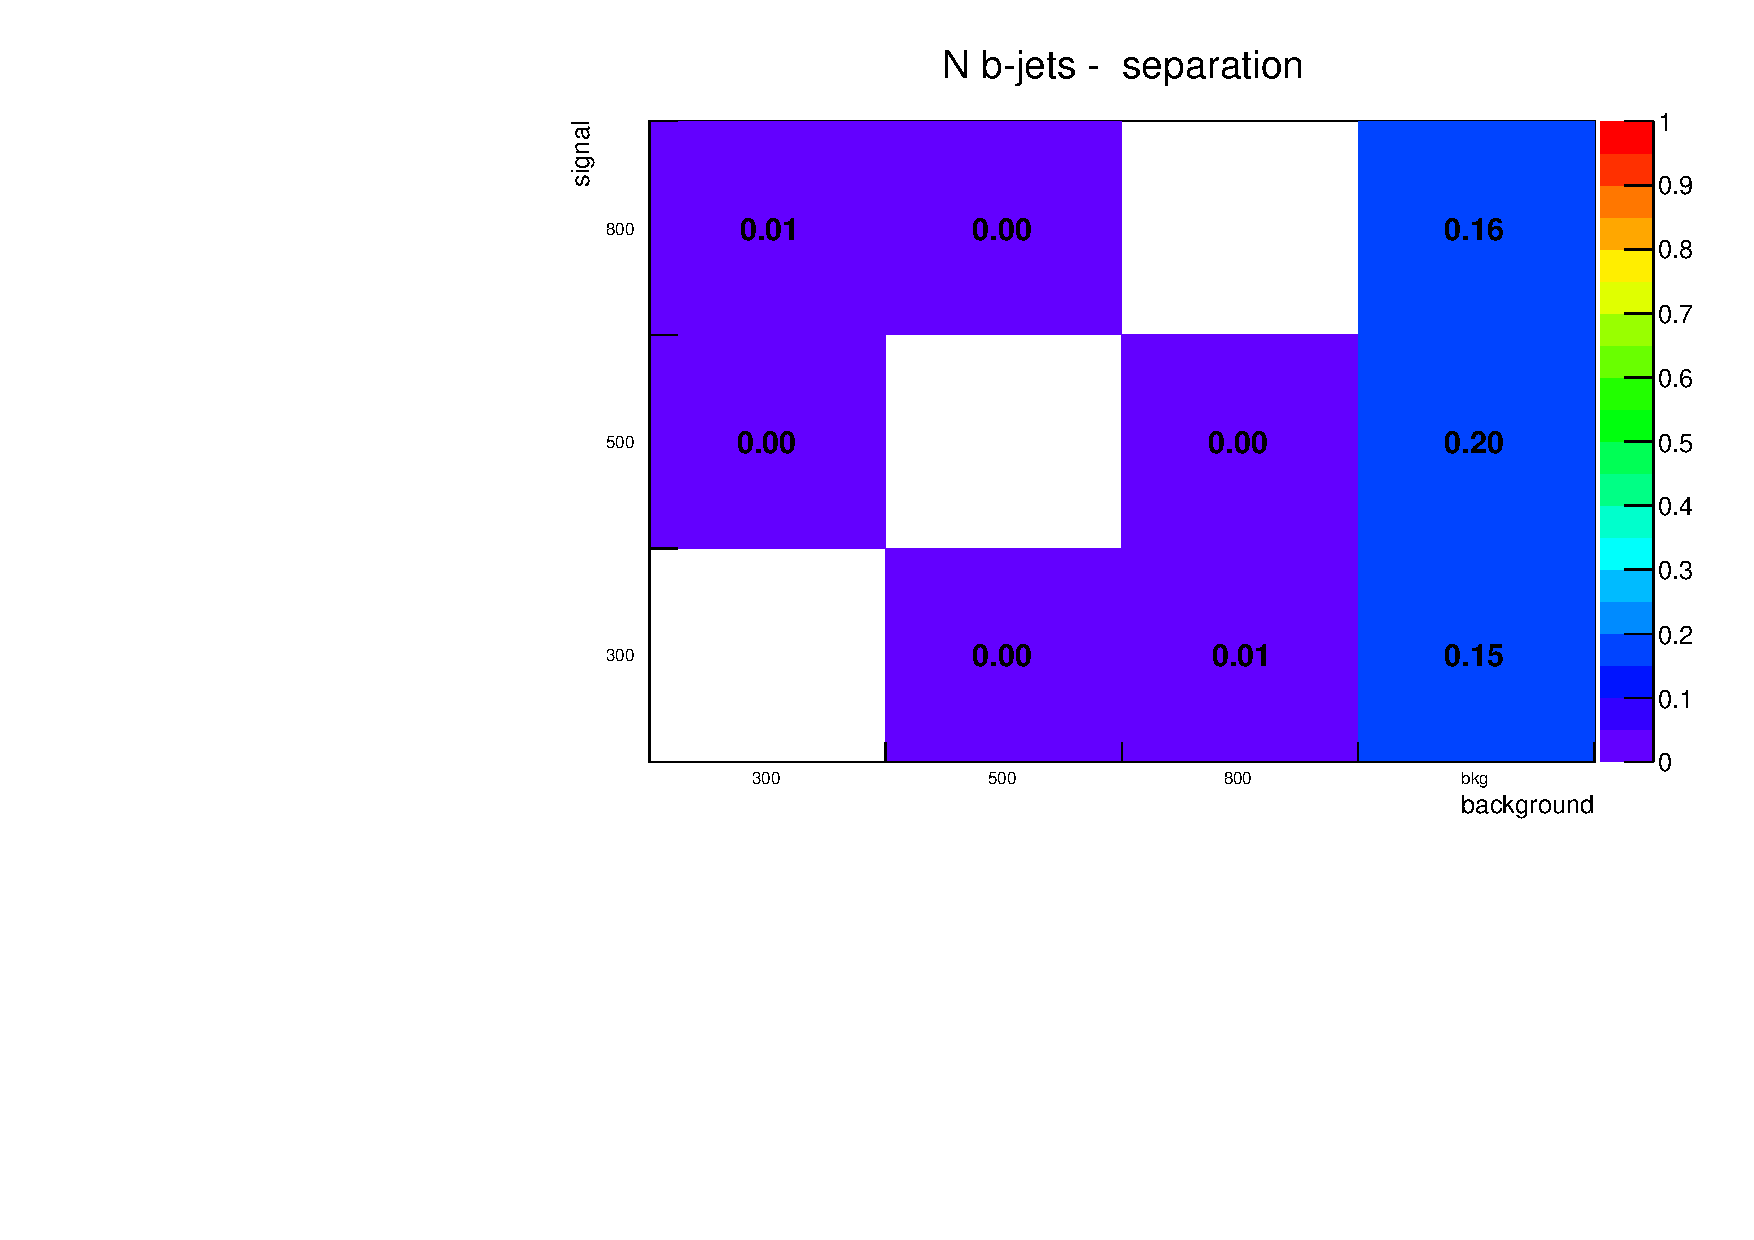
\includegraphics[width=0.43\textwidth]{figures/ewk_prod/separation/saparation_Nb_jets.pdf}}\\
\subfigure[]{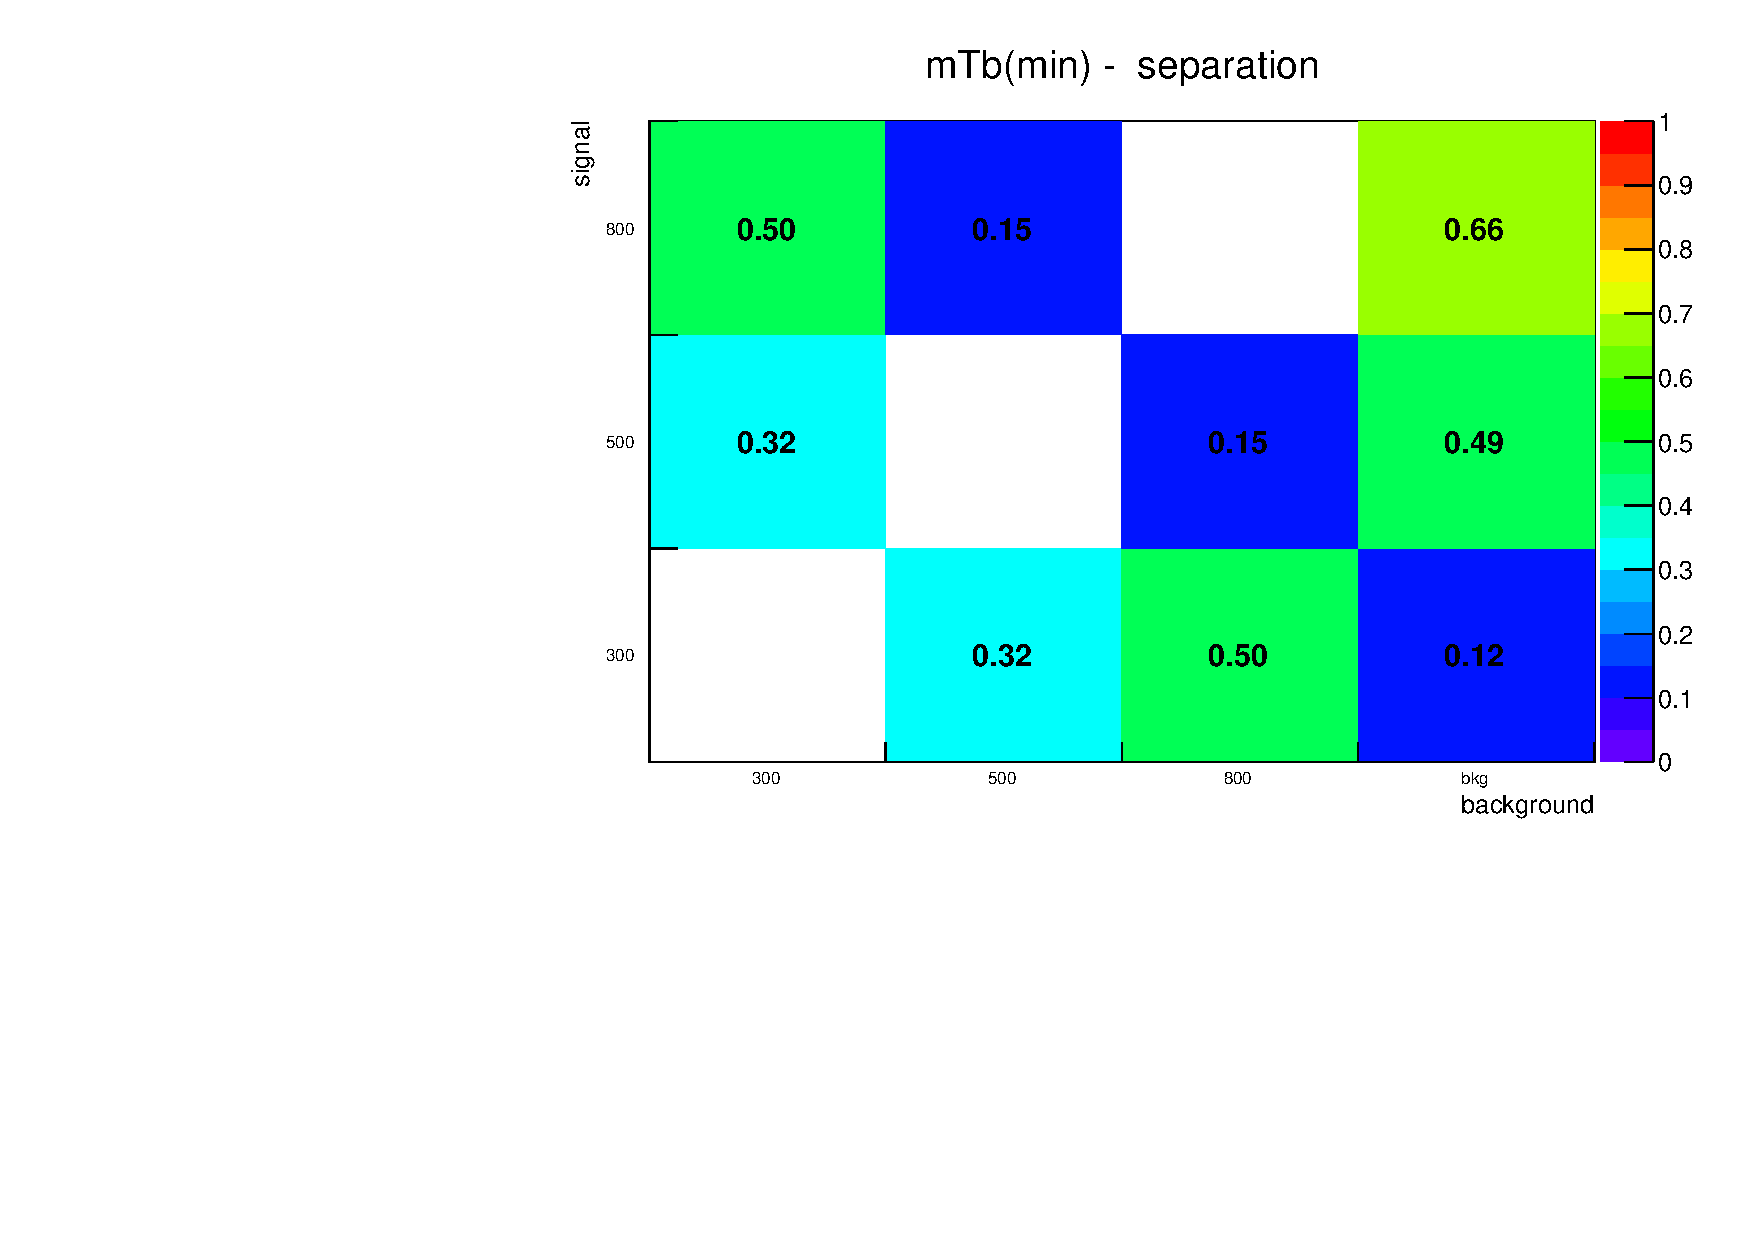
\includegraphics[width=0.43\textwidth]{figures/ewk_prod/separation/saparation_mTbmin.pdf}}
\subfigure[]{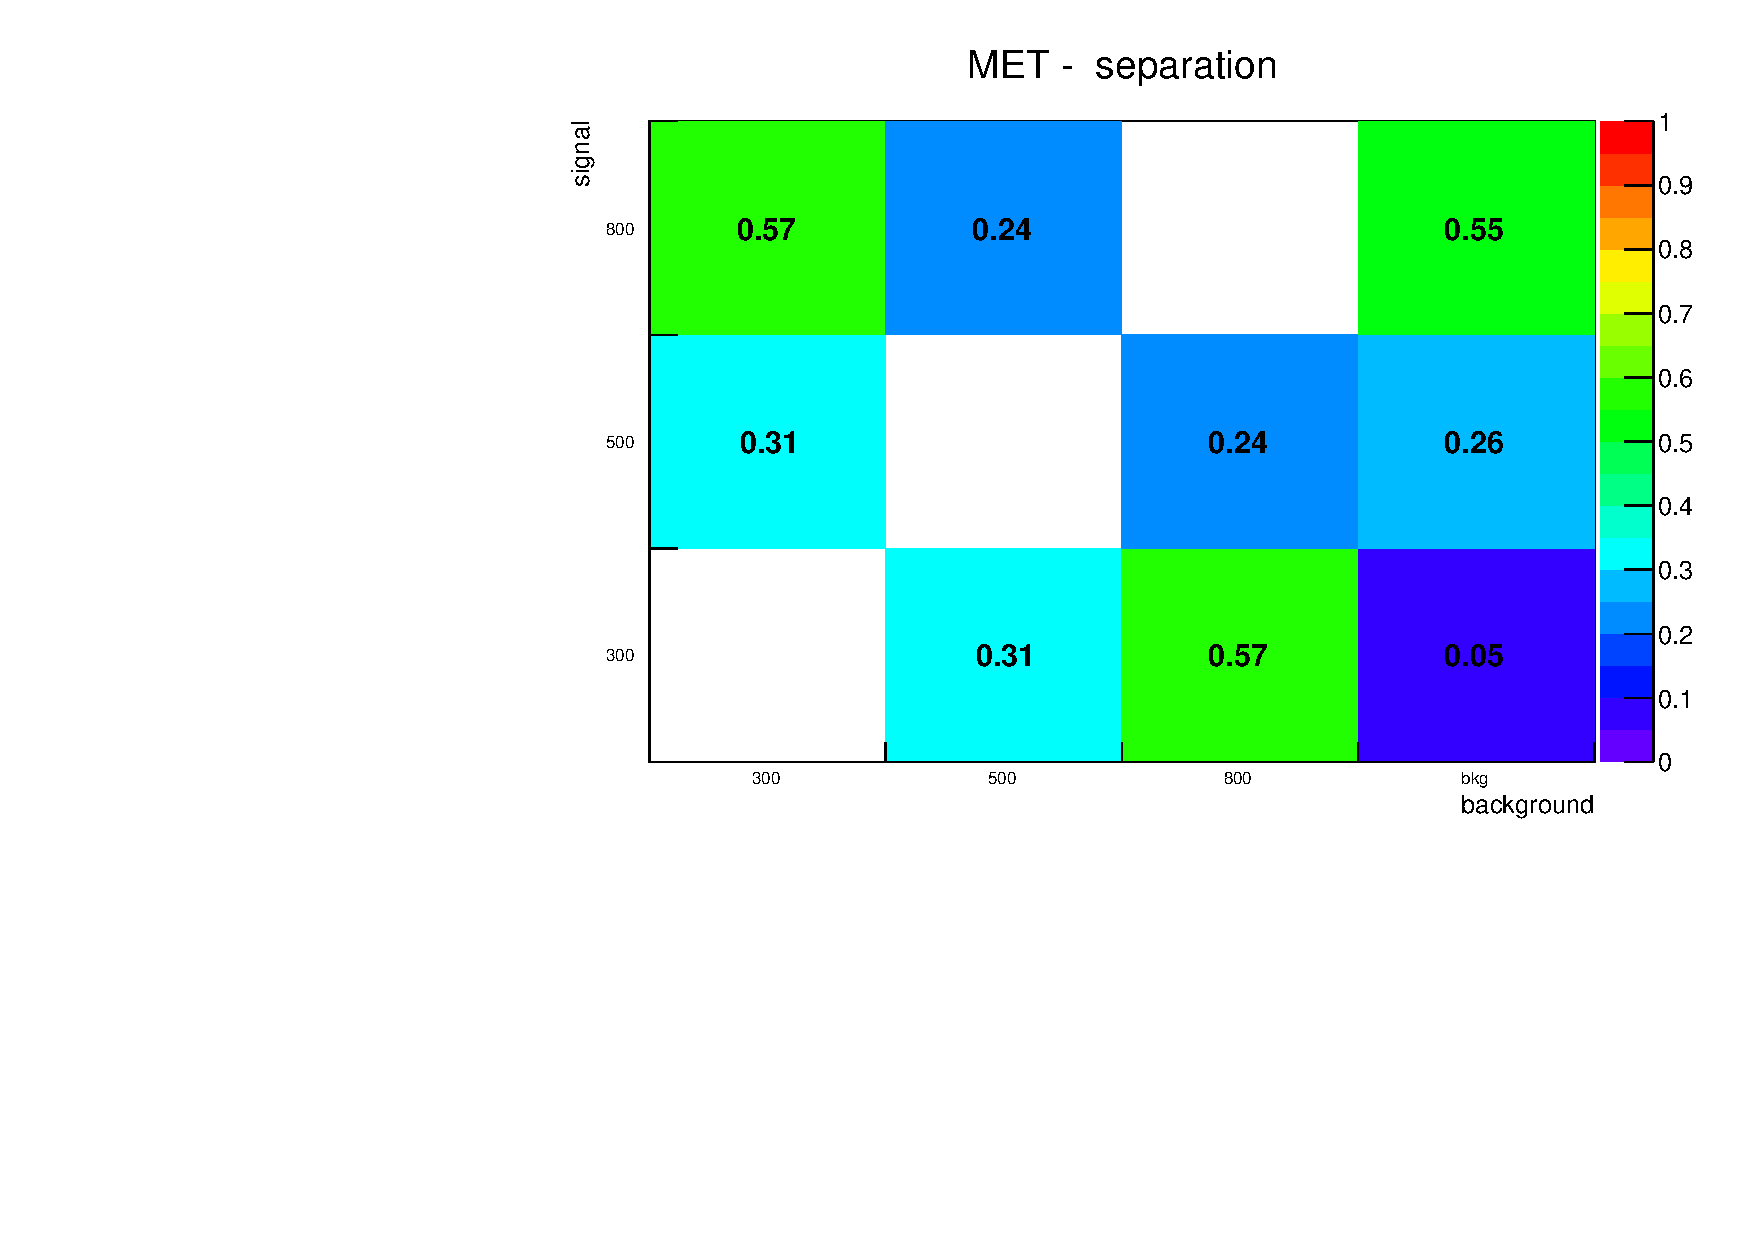
\includegraphics[width=0.43\textwidth]{figures/ewk_prod/separation/saparation_MET.pdf}}\\
%\subfigure[]{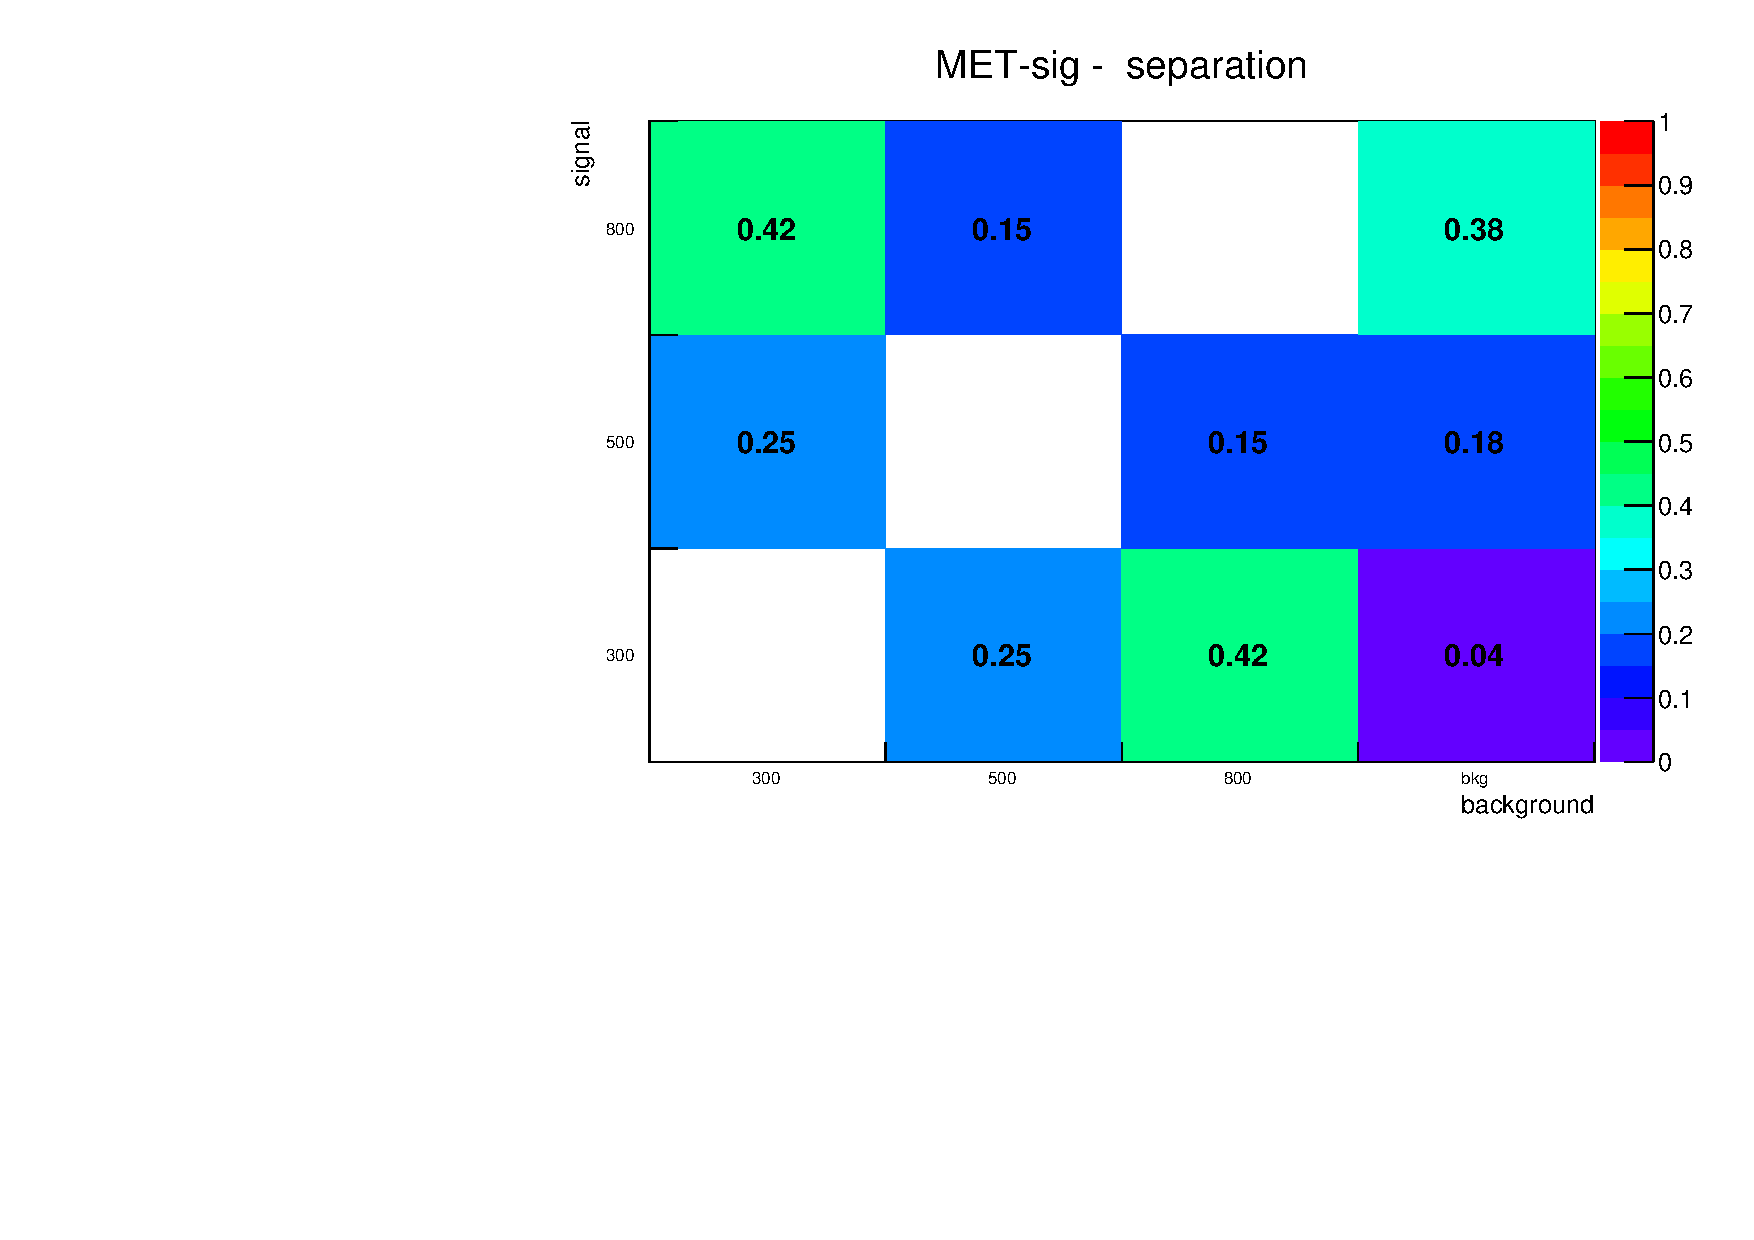
\includegraphics[width=0.43\textwidth]{figures/ewk_prod/separation/saparation_MET_sig.pdf}}
\caption{Separation offered by different analysis variables. The separation is defined as in Equation \ref{eq:separation}.}
\label{fig:ewk:separation}
\end{center}
\end{figure}

Three regular bins with a width of 150 GeV each are defined in \meffb. 
The edges of the bins are defined starting from the one with the highest value. 
At it has already been discussed in Section \ref{sec:ewk:sigbkg},
signals with high m(\hino) have kinematic features that distinguish them clearly from the background, 
but at the same time a low cross-section (e.g. for m($\ninoone$) = 800 GeV, the cross-section is about 3 fb). 
This makes it more convenient to define the selection that maximize the expected significance for a high-mass benchmark point (800 GeV) 
as a single-bin region, to concentrate as much as possible the signal events in one single \gls{sr}, 
instead of diluting it in several \glspl{sr}. % to try to exploit shape information.
The optimal selection for the high-m(\hino) benchmark signal occupies the highest \meffb bin,
and is determined my maximizing the expected significance over all the other discriminating variables,
leading to the selection:
\meffb $>$ 1100 GeV, \mtb$>$130 GeV, \dRmax $<$ 1.4, \met $>$200, $\geq$ 3 $b$-jets (77\% \gls{op}), 
4-5 jets, m($h_1$) in the range 110-150 GeV, m($h_2$) in the range 90-140 GeV.

Considering the separation power of the different variables shown in Figure  \ref{fig:ewk:separation} 
and the signal-to-background comparison in Figure \ref{fig:ewk:sig:1}, 
\dRmax is chosen as second binning variable. 
%to gain signal acceptance also for signals less boosted than the 800 GeV mass one, where the angular separation between the two $b$-jets originating from the same higgs is larger.
Once the selections for the high-\meffb \gls{sr} have been defined, 
a similar procedure is repeated for the other \meffb ranges: 600-850 GeV and 850-1100 GeV. 
These two bins with lower \meffb are also split according to the number of $b$-jets: exactly 3 and $\geq$4. 
The two bins in $b$-jet multiplicity are optimized separately. 
For each of the four remaining regions, the following steps are taken:

\begin{enumerate}
\item Optimize for one specific signal benchmark: \mhino = 300, 500 GeV for the 600-850 and 850-1100 GeV \meffb bins respectively.
\item  Where possible with a loss in significance $<$ 15\%, the selections are made uniform. 
This results to be the case for the m($h_1$) and m($h_2$) ranges, for the selection in \met, for the first bin in \dRmax, 
and for the number of jets. In the case of this last variable, it is possible to make it uniform (4-5 jets) 
without consistent loss in sensitivity in all bins except in the 4b-meff2 bin, where a veto on a 6th jet is penalizing; 
in this region, the selection on the number of jets is 4-6.
\item Use \dRmax to define further bins.
\end{enumerate}

It is found that a second bin in \dRmax is really helpful only in the regions with low and intermediate \meffb, and  $\geq$ 4 $b$-jets. 
This is because the highest \meffb region is particularly sensitive to high-mass signals, where \dRmax is small. 
For signals with lower masses, the signal-to-background ratio in regions with exactly 3 $b$-jets and high \dRmax is too low, 
while the requirement of a fourth $b$-jet suppresses the \gls{sm} background further and gives good sensitivity 
also to the region of phase space with higher \dRmax.
The final \glspl{sr} selections are summarized in Table \ref{tab:SR}.

\begin{table}[htbp]
\begin{center}
%\resizebox{1.\textwidth}{!}{
\renewcommand{\arraystretch}{1.1}
\begin{tabular}{|l|c|c|c|}
\toprule
  & SR-3b-meff1-A & SR-3b-meff2-A & SR-3b-meff3-A\\
 \hline
\nbjet &  $=$3 &  $=$3 &  $\geq$3 \\
 \hline
\met & \multicolumn{3}{|c|}{$>$ 200}\\
\hline
\dphimin    & \multicolumn{3}{|c|}{$>$0.4}\\
 \hline
\njet &  4--5 &  4--5 &  4--5 \\
 \hline
\mtb &  $>$150 &  $>$150 &  $>$130 \\
 \hline
$m(h_1)$ &    \multicolumn{3}{|c|}{110--150}\\
 \hline
$m(h_2)$ &    \multicolumn{3}{|c|}{90--140}\\
 \hline
\dRmax &  0.4--1.4 &  0.4--1.4 &  0.4--1.4 \\
 \hline
\meffb &  600--850 &  850--1100 &  $>$1100  \\
\bottomrule
\end{tabular} 

\vspace{0.4cm}

\begin{tabular}{|l|c|c|c|c|}
\toprule
   & SR-4b-meff1-A & SR-4b-meff1-B & SR-4b-meff2-A & SR-4b-meff2-B  \\
 \hline
\nbjet &  $\geq$4 &  $\geq$4 &  $\geq$4 &  $\geq$4 \\
 \hline
\met & \multicolumn{4}{|c|}{$>$ 200}\\
\hline
\dphimin    & \multicolumn{4}{|c|}{$>$0.4}\\
 \hline
\njet & 4--5 &  4--5 &  4--6 &  4--6 \\
 \hline
\mtb &   - & - & - & -  \\
 \hline
$m(h_1)$ &    \multicolumn{4}{|c|}{110--150}\\
 \hline
$m(h_2)$ &    \multicolumn{4}{|c|}{90--140}\\
 \hline
\dRmax &   0.4--1.4 &  1.4--2.4 &  0.4--1.4 &  1.4--2.4\\
 \hline
\meffb &  600--850 &  600--850 &  850--1100 &  850--1100 \\
\bottomrule
\end{tabular} 
%}
\caption{Signal region definitions for the high-mass analysis. The units of \met, \mtb, $m(h_1)$, $m(h_2)$, and \meffb are GeV. 
Table from Ref. \cite{Aaboud:2018htj}.
%These variables are defined in Section~\ref{high_event_selection}.
}
\label{tab:SR}
\end{center}
\end{table}

\subsection{Cut-and-count regions}

The analysis strategy described in Section \ref{sec:ewk:multibin} leads to a good sensitivity for exclusion across the entire mass spectrum, 
but the constraint of building orthogonal regions makes it hard to have a high discovery significance 
for signals with intermediate masses. 
To solve this problem cut-and-count \glspl{sr} are defined as well, with the goal of
providing robust regions capable of discovery of \gls{susy} signatures, 
and allowing an easier reinterpretation of the results.

The upper selection on \meffb, that makes the different \glspl{sr} orthogonal, 
is the one limiting the most the sensitivity of the individual \glspl{sr}.
In the exclusion fit this is not a problem, as the sensitivity lost in one bin is recovered in the neighbouring one. 
To define the discovery regions, all the individual \glspl{sr} are considered without the upper cut on \meffb
and the expected significance for some benchmark signal models is computed in each. 
The expected significance is computed as discussed in Section \ref{sec:example_sr}, 
assuming 36.1 \ifb of data and a flat 30\% background uncertainty. 

Figure \ref{fig:ewk:disc_sig} shows the expected significance for all the multi-bin analysis regions once the upper \meffb 
selection is removed. 
Using only the modified versions of SR-4b-meff1-A, referred to as SR-4b-meff1-A-disc, 
and SR-3b-meff3 (orange and green line respectively in the figure) allow us to have good expected sensitivity for 
all the signal considered.  
This is always $>$3 standard deviations for all the masses in the 300-600 GeV range, and $\approx$ 2.5 standard deviations for the 800 GeV signal. 
The definition of SR-4b-meff1-A-disc is reported in Table \ref{tab:SR-disc}.

\begin{figure*}[htbp]
\centering
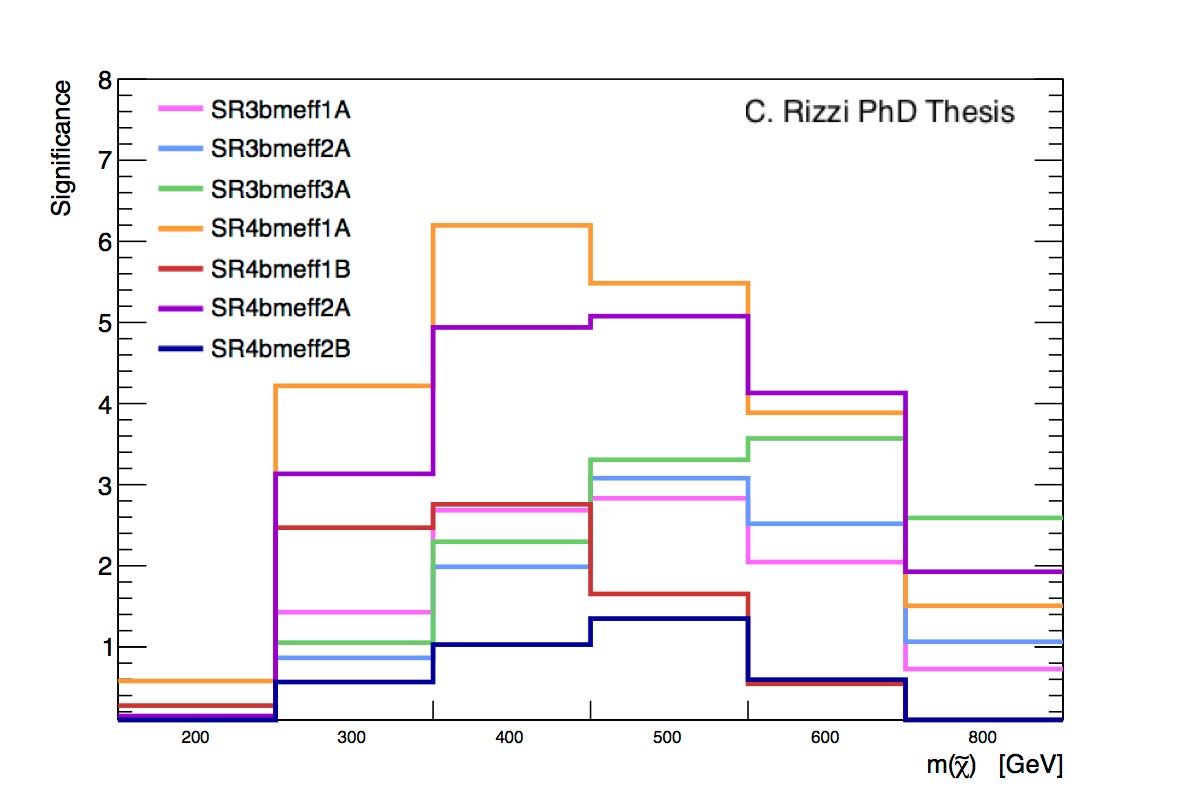
\includegraphics[width=0.7\textwidth]{figures/ewk_prod/discovery/significances_hh_regions.pdf}
\caption{Expected significance for the multi-bin regions after removing the upper \meffb selection. 
\label{fig:ewk:disc_sig}
}
\end{figure*}

\begin{table}[htbp]
\begin{center}
\renewcommand{\arraystretch}{1.1}
\begin{tabular}{|l|c|}
\toprule
   & SR-4b-meff1-A-disc \\
 \hline
\nbjet &  $\geq4$\\
 \hline
\met & $>$ 200\\
\hline
\dphimin    &$>$0.4\\
 \hline
\njet &  4--5\\
 \hline
\mtb &  - \\
 \hline
$m(h_1)$ &    110--150\\
 \hline
$m(h_2)$ &   90--140\\
 \hline
\dRmax &  0.4--1.4 \\
 \hline
\meffb &  $>600$ \\
\bottomrule
\end{tabular} 
%}
\caption{Definition of the high-mass analysis  SR-4b-meff1-A-disc. The units of \met, \mtb, $m(h_1)$, $m(h_2)$, and \meffb are GeV. 
Table from Ref. \cite{Aaboud:2018htj}.
%These variables are defined in Section~\ref{high_event_selection}.
}
\label{tab:SR-disc}
\end{center}
\end{table}


\section{Control and validation regions}
\label{sec:ewk:CRVR}

The \ttbar background is normalized in specifically designed \glspl{cr}.
A different \gls{cr} is built for each bin in \meffb and $b$-tagging multiplicity. 
These \glspl{cr} are built using side-bands both in m($h_1$) and m($h_2$). 
The extrapolation between \glspl{cr} and \glspl{sr} is tested in the \glspl{vr}, which take advantage of events
where only one between m($h_1$) and m($h_2$) is in the \gls{sr} mass range, 
as shown in Figure \ref{fig:binning_crvr}.

\begin{figure}[htbp]
	\centering
	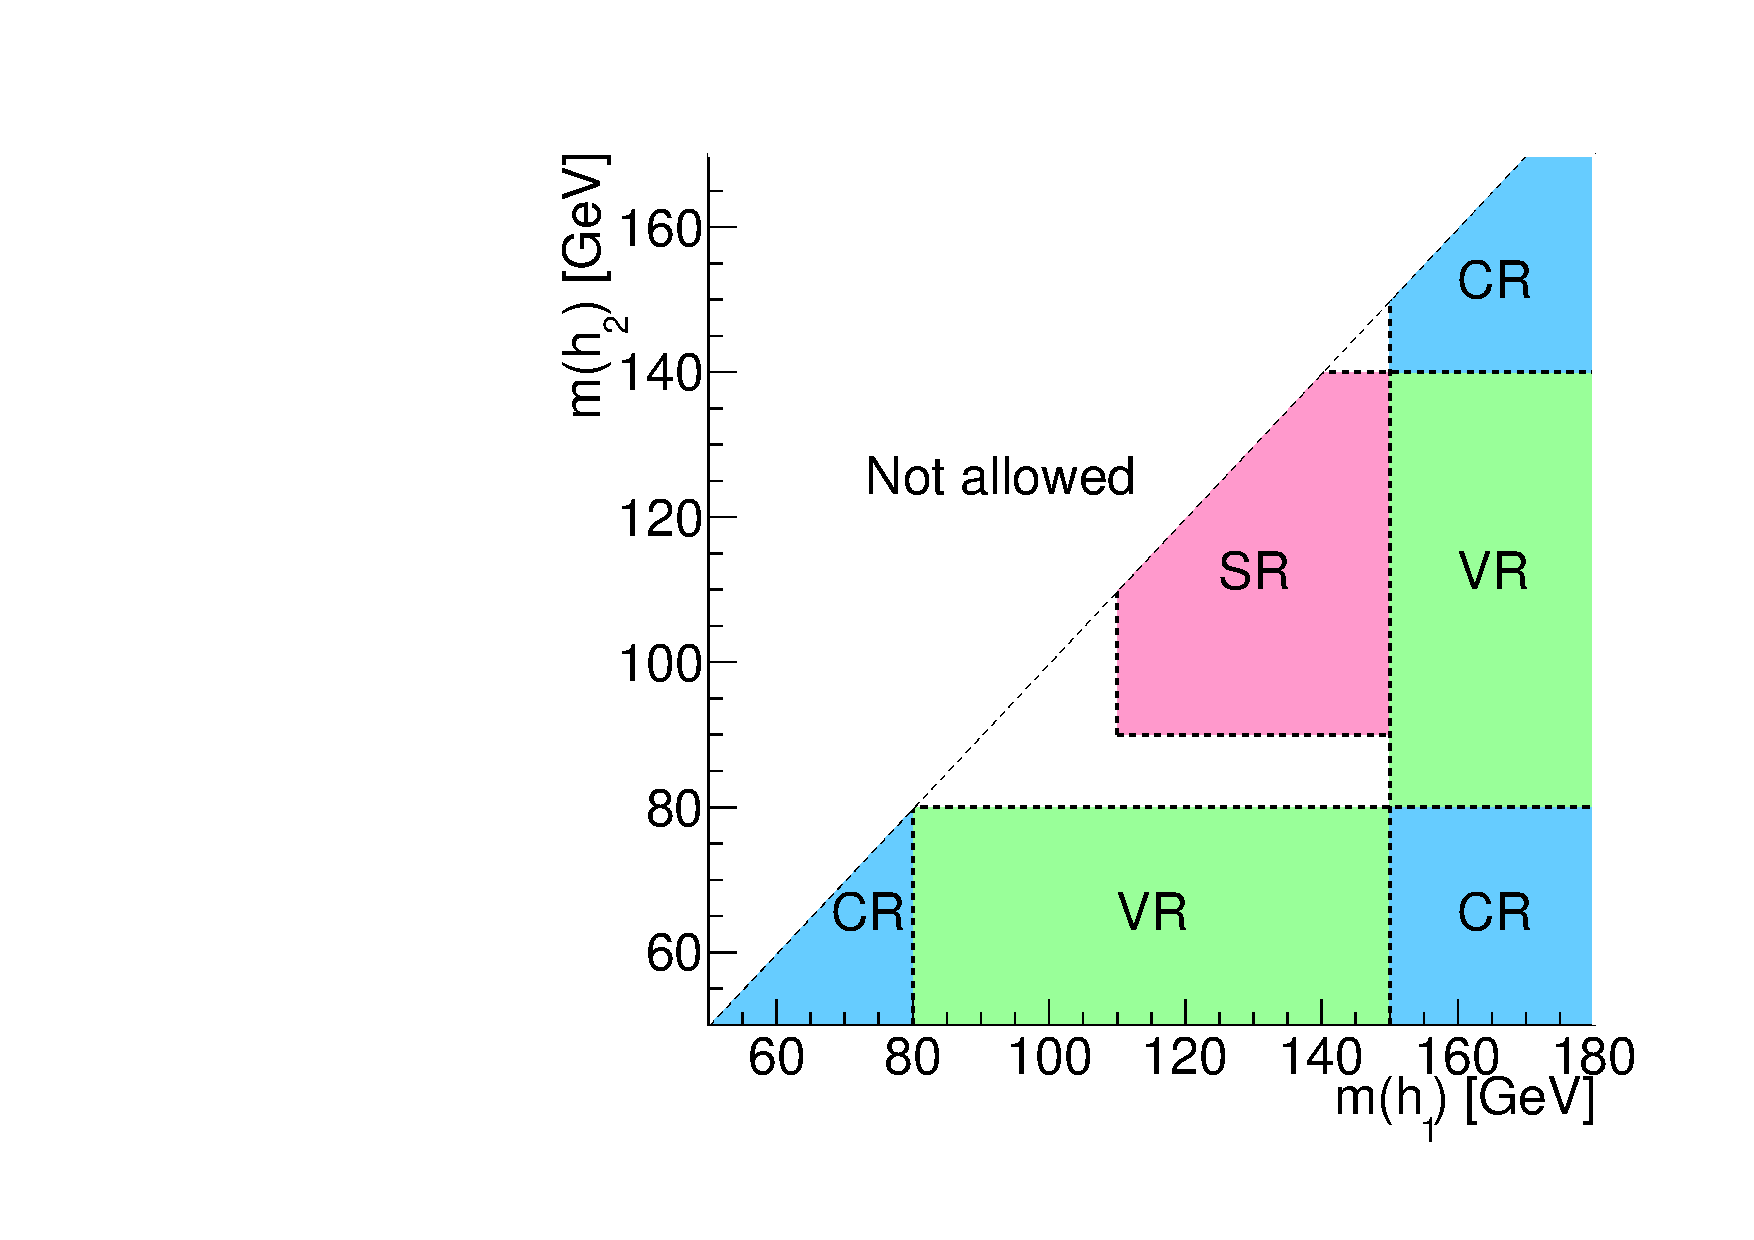
\includegraphics[width=0.490\textwidth]{figures/ewk_prod/varie/schema-1}
	\caption{The division of signal, control, and validation regions using the $m(h_1)$ and $m(h_2)$ variables in the high-mass analysis.}
	\label{fig:binning_crvr}
\end{figure}

Some of the selections of the \glspl{sr} are modified when moving to the \glspl{cr} or \glspl{vr}
 to allow enough events and low signal contamination.
The main extrapolation between \glspl{cr} and \glspl{sr} are:

\begin{itemize}
\item In the \gls{cr}, both m($h_1$) and m($h_2$) are required to be outside the \gls{sr} mass ranges.
\item \dRmax is relaxed to $<$4 (or removed).
\item \mtb is relaxed by 30 GeV in 3b-meff3 and by 50 GeV in 3b-meff1 and 3b-meff2.
\end{itemize}

To allow enough events in the \glspl{vr}, the \glspl{vr} are non orthogonal. Since these regions do not enter the fit, but are only used to validate the background prediction, non-orthogonality is not an issue here. 
The selections that remove the orthogonality between the different \glspl{vr} are:
\begin{itemize}
\item The edges of \meffb selection are relaxed by 50 GeV up and down.
\item The edges of the \dRmax bins are relaxed and, when two \dRmax bins are present for the same type of regions, they are partially overlapping.
\end{itemize}

With respect to the \glspl{sr}, the \mtb selection (where present) is relaxed as well by 50 GeV. 
Note that \glspl{cr} and \glspl{vr} do not have extrapolation in \nbjet or \njet with respect to the SRs.
The selections for all the \glspl{cr} and \glspl{vr} are summarized respectively in Tables \ref{tab:ewk:CR} and \ref{tab:ewk:VR}.


\begin{table}[htbp]
\begin{center}
%\resizebox{0.75\textwidth}{!}{
\renewcommand{\arraystretch}{1.1}
\begin{tabular}{|l|c|c|c|c|c|}
\toprule
  & CR-3b-meff1 & CR-3b-meff2 & CR-3b-meff3 & CR-4b-meff1 & CR-4b-meff2 \\
 \hline
\nbjet &  $=$3 &  $=$3 &  $\geq$3 &  $\geq$4 &  $\geq$4 \\
 \hline
\met  & \multicolumn{5}{|c|}{$>$ 200}\\
 \hline
\dphimin  & \multicolumn{5}{|c|}{$>$0.4}\\
 \hline
\njet &  4--5 &  4--5 &  4--5 &  4--5 &  4--6 \\
 \hline
\mtb &  $>$100 &  $>$100 &  $>$100 & - & - \\
 \hline
$m(h_1)$, $m(h_2)$  &  \multicolumn{5}{|c|}{ ($m(h_1)<$80, $m(h_2)<$80) or ($m(h_1)>$150, $m(h_2)<$80) or ($m(h_1)>$150, $m(h_2)>$140)    }\\
 \hline
\dRmax &  0.4--4 &  0.4--4 &  0.4--4 &  0.4--4 &  $\geq$ 0.4 \\
 \hline
\meffb &  600--850 &  850--1100 &  $>$1100 &  600--850 &  850--1100 \\
\bottomrule
\end{tabular} 
%} 
\caption{Control region definitions in the high-mass analysis. The units of \met, \mtb, $m(h_1)$, $m(h_2)$, and \meffb are GeV. 
Table from Ref. \cite{Aaboud:2018htj}.
%These variables are defined in Section~\ref{high_event_selection}.
}
\label{tab:ewk:CR}
\end{center}
\end{table}

\begin{table}[htbp]
\begin{center}
\renewcommand{\arraystretch}{1.1}
%\resizebox{1\textwidth}{!}{
\begin{tabular}{|l|c|c|c|}
\toprule
  & VR-3b-meff1-A & VR-3b-meff2-A & VR-3b-meff3-A \\
 \hline
\nbjet &  $=$3 &  $=$3 &  $\geq$3  \\
 \hline
\met  &  \multicolumn{3}{|c|}{$>$200}\\
 \hline
\dphimin &  \multicolumn{3}{|c|}{$>$0.4}\\
 \hline
\njet &  4--5 &  4--5 &  4--5 \\
 \hline
\mtb  & $>$120   & $>$100  & $>$80 \\
 \hline
$m(h_1)$, $m(h_2)$  &  \multicolumn{3}{|c|}{   (80<$m(h_1)$<150, $m(h_2)$<80) or ($m(h_1)$>150, 90<$m(h_2)$<140)   }\\
 \hline
\dRmax &  0.4--1.5 &  0.4--1.7 &  0.4--1.7  \\
 \hline
\meffb   & 550--900   & 800--1150  & $>$1050    \\
\bottomrule
\end{tabular} 

\vspace{0.4cm}

\begin{tabular}{|l|c|c|c|c|}
\toprule
  &  VR-4b-meff1-A & VR-4b-meff1-B & VR-4b-meff2-A & VR-4b-meff2-B \\
 \hline
\nbjet &   $\geq$4 &  $\geq$4 &  $\geq$4 &  $\geq$4 \\
 \hline
\met  &  \multicolumn{4}{|c|}{$>$200}\\
 \hline
\dphimin &  \multicolumn{4}{|c|}{$>$0.4}\\
 \hline
\njet &   4--5 &  4--5 &  4--6 &  4--6 \\
 \hline
\mtb   &  \multicolumn{4}{|c|}{-}\\
 \hline
$m(h_1)$, $m(h_2)$  &  \multicolumn{4}{|c|}{   (80<$m(h_1)$<150, $m(h_2)$<80) or ($m(h_1)$>150, 90<$m(h_2)$<140)   }\\
 \hline
\dRmax &   0.4--1.7 &  1.4--3 &  0.4--1.7 &  1.4--3 \\
 \hline
\meffb   &  550--900  & 550--900  & 800--1150  & 800--1150  \\
\bottomrule
\end{tabular} 
%} 
\caption{Validation region definitions in the high-mass analysis. The units of \met, \mtb, $m(h_1)$, $m(h_2)$, and \meffb are GeV. 
Table from Ref. \cite{Aaboud:2018htj}.
%These variables are defined in Section~\ref{high_event_selection}.
}
\label{tab:ewk:VR}
\end{center}
\end{table}

\section{Background composition}
\label{sec:ewk:bkgcomp}

The pre-fit background composition of the analysis regions is show in Figures \ref{fig:bkgcomp_hh3b} and \ref{fig:bkgcomp_hh4b}.
It is possible to see how \ttbar is the dominant background in all the \glspl{sr}.
%The \glspl{cr} and the \glspl{vr} have a high \ttbar purity by construction. 
%, since they are designed to respectively normalize this background and validate the extrapolation of this normalization to 
%a phase space closer to the \glspl{sr}.
% chiara: change, sentence from paper
The subdominant background contributions are $Z(\to \nu\nu)$+jets and $W(\to \ell\nu)$+jets events.
%where for W+jets events the lepton is electron or muon that is not reconstructed or a hadronically decaying $\tau$-lepton. 
%In the 1-lepton \glspl{sr}, the subdominant backgrounds are single-top, \ttbar+W and \ttbar+Z.
Figures \ref{fig:ttcomp_hh3b} and \ref{fig:ttcomp_hh3b} show the decay type of the \ttbar background,
while the heavy-flavor composition of the jets that are produced together with the \ttbar pair is shown 
in Figures \ref{fig:HFcomp_hh3b} and \ref{fig:HFcomp_hh3b}.

\begin{figure}[htbp]
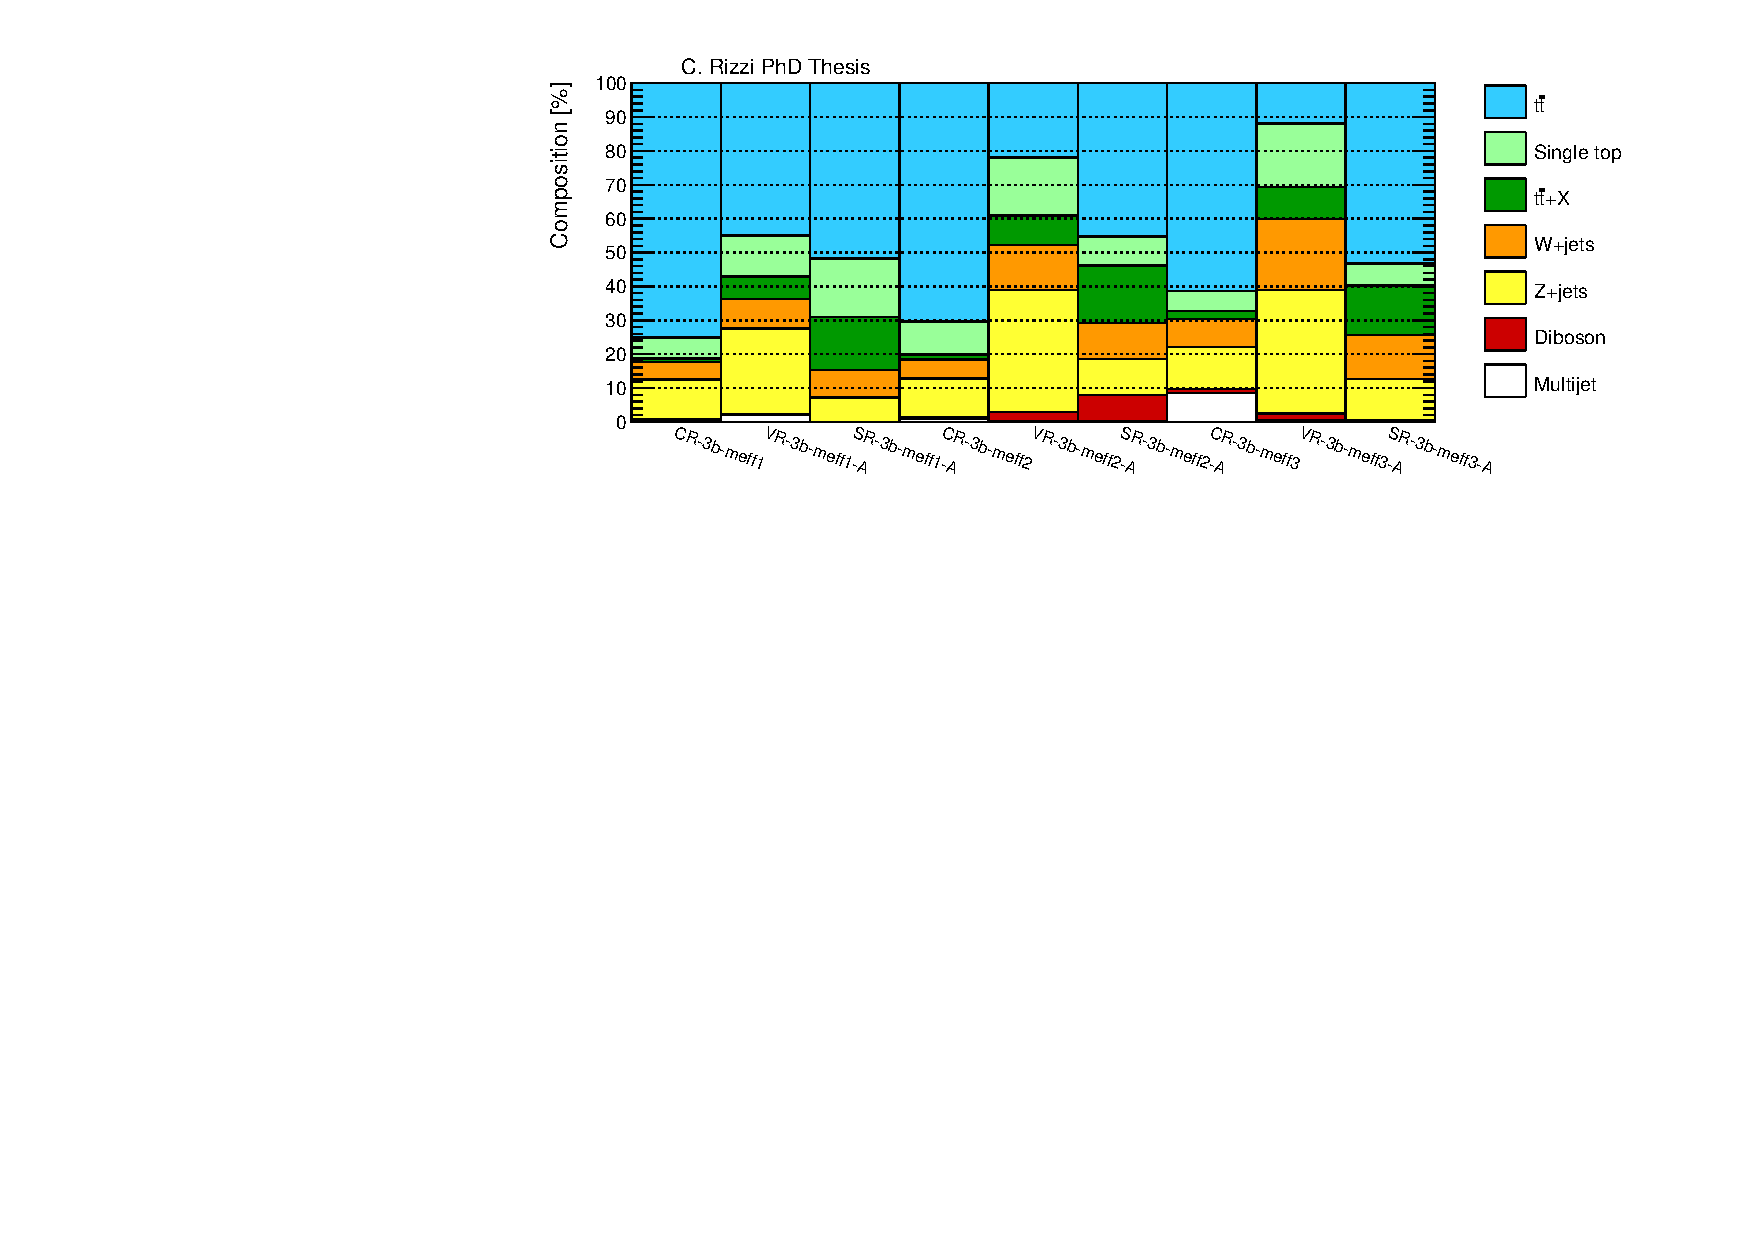
\includegraphics[width=\textwidth]{figures/ewk_prod/comp_plots/hh_3b_bkg.pdf}
\caption{Background composition in the regions with exactly three $b$-jets.}
	\label{fig:bkgcomp_hh3b}
\end{figure}

\begin{figure}[htbp]
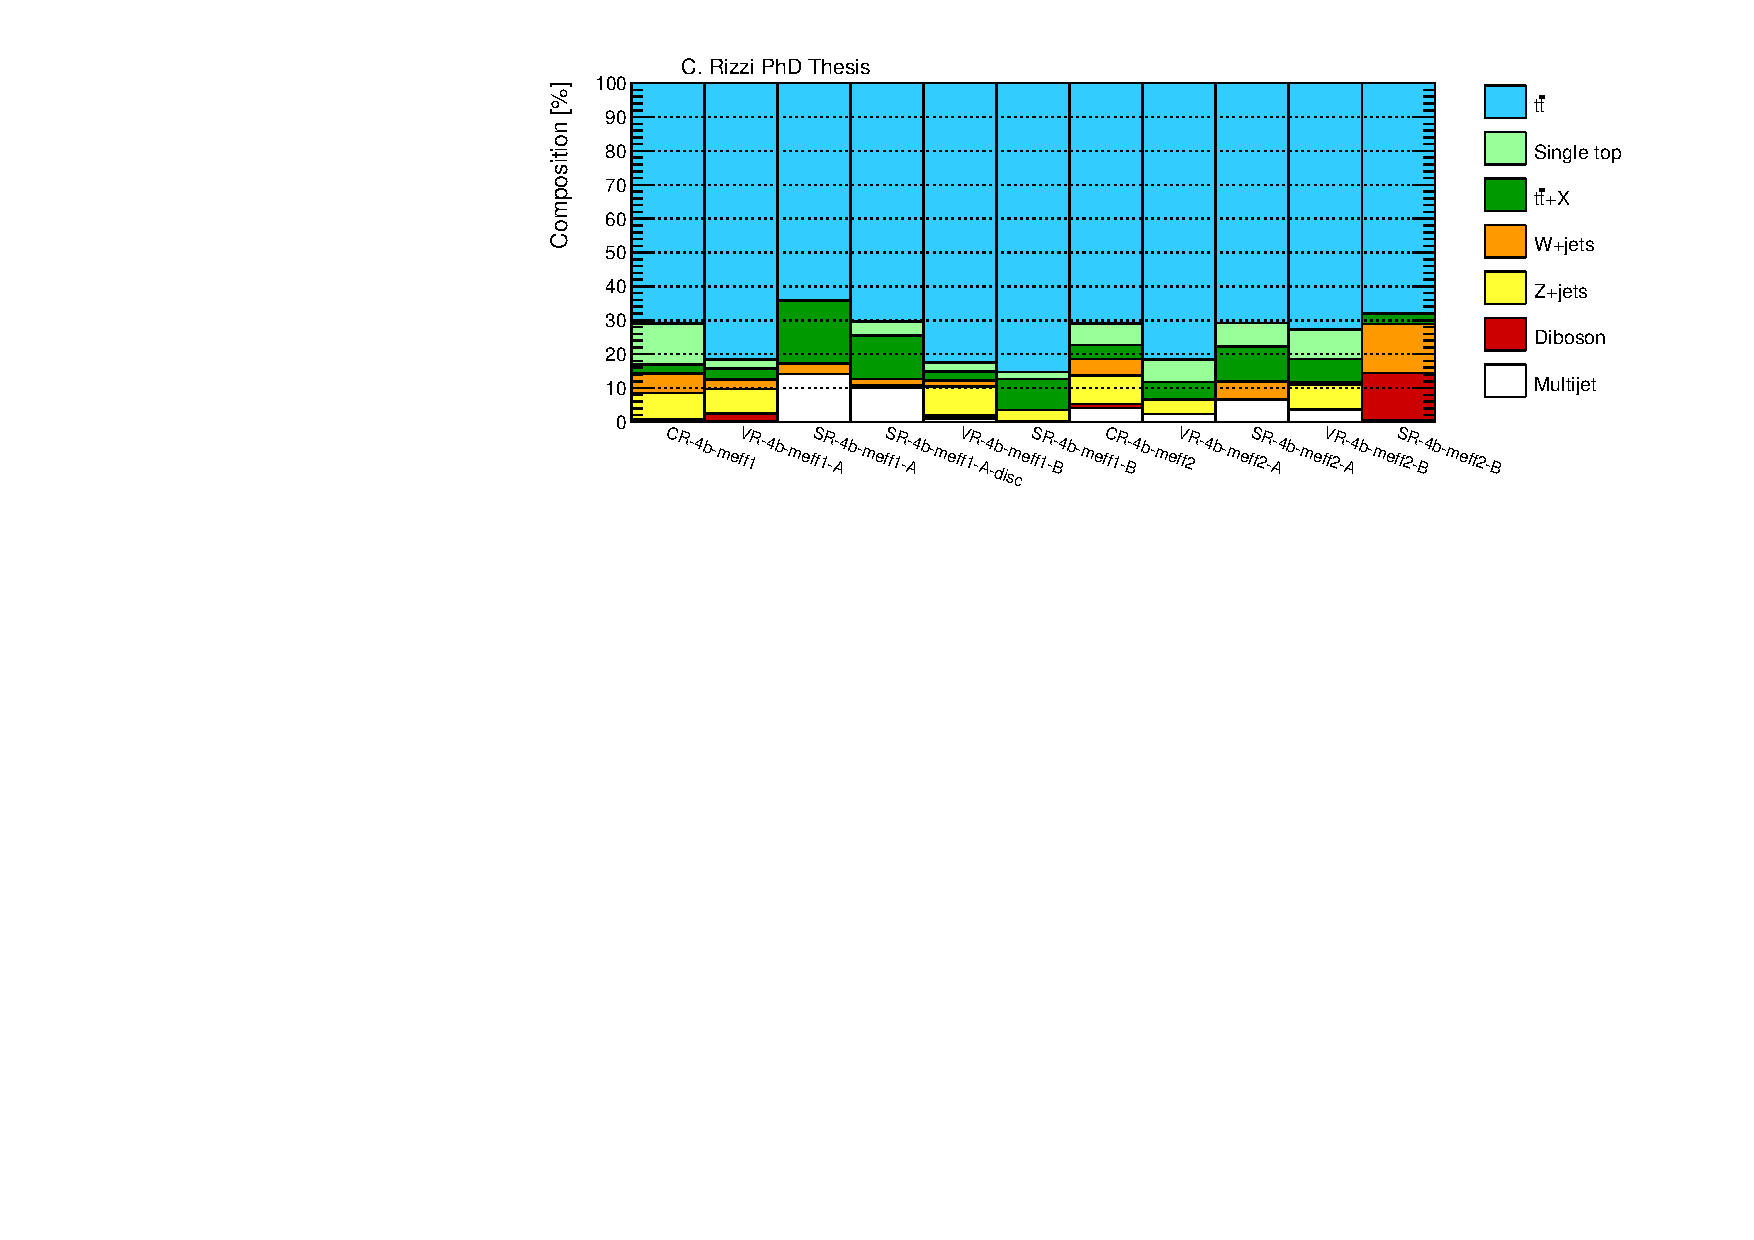
\includegraphics[width=\textwidth]{figures/ewk_prod/comp_plots/hh_4b_bkg.pdf}
\caption{Background composition in the regions with at least four $b$-jets.}
	\label{fig:bkgcomp_hh4b}
\end{figure}

\begin{figure}[htbp]
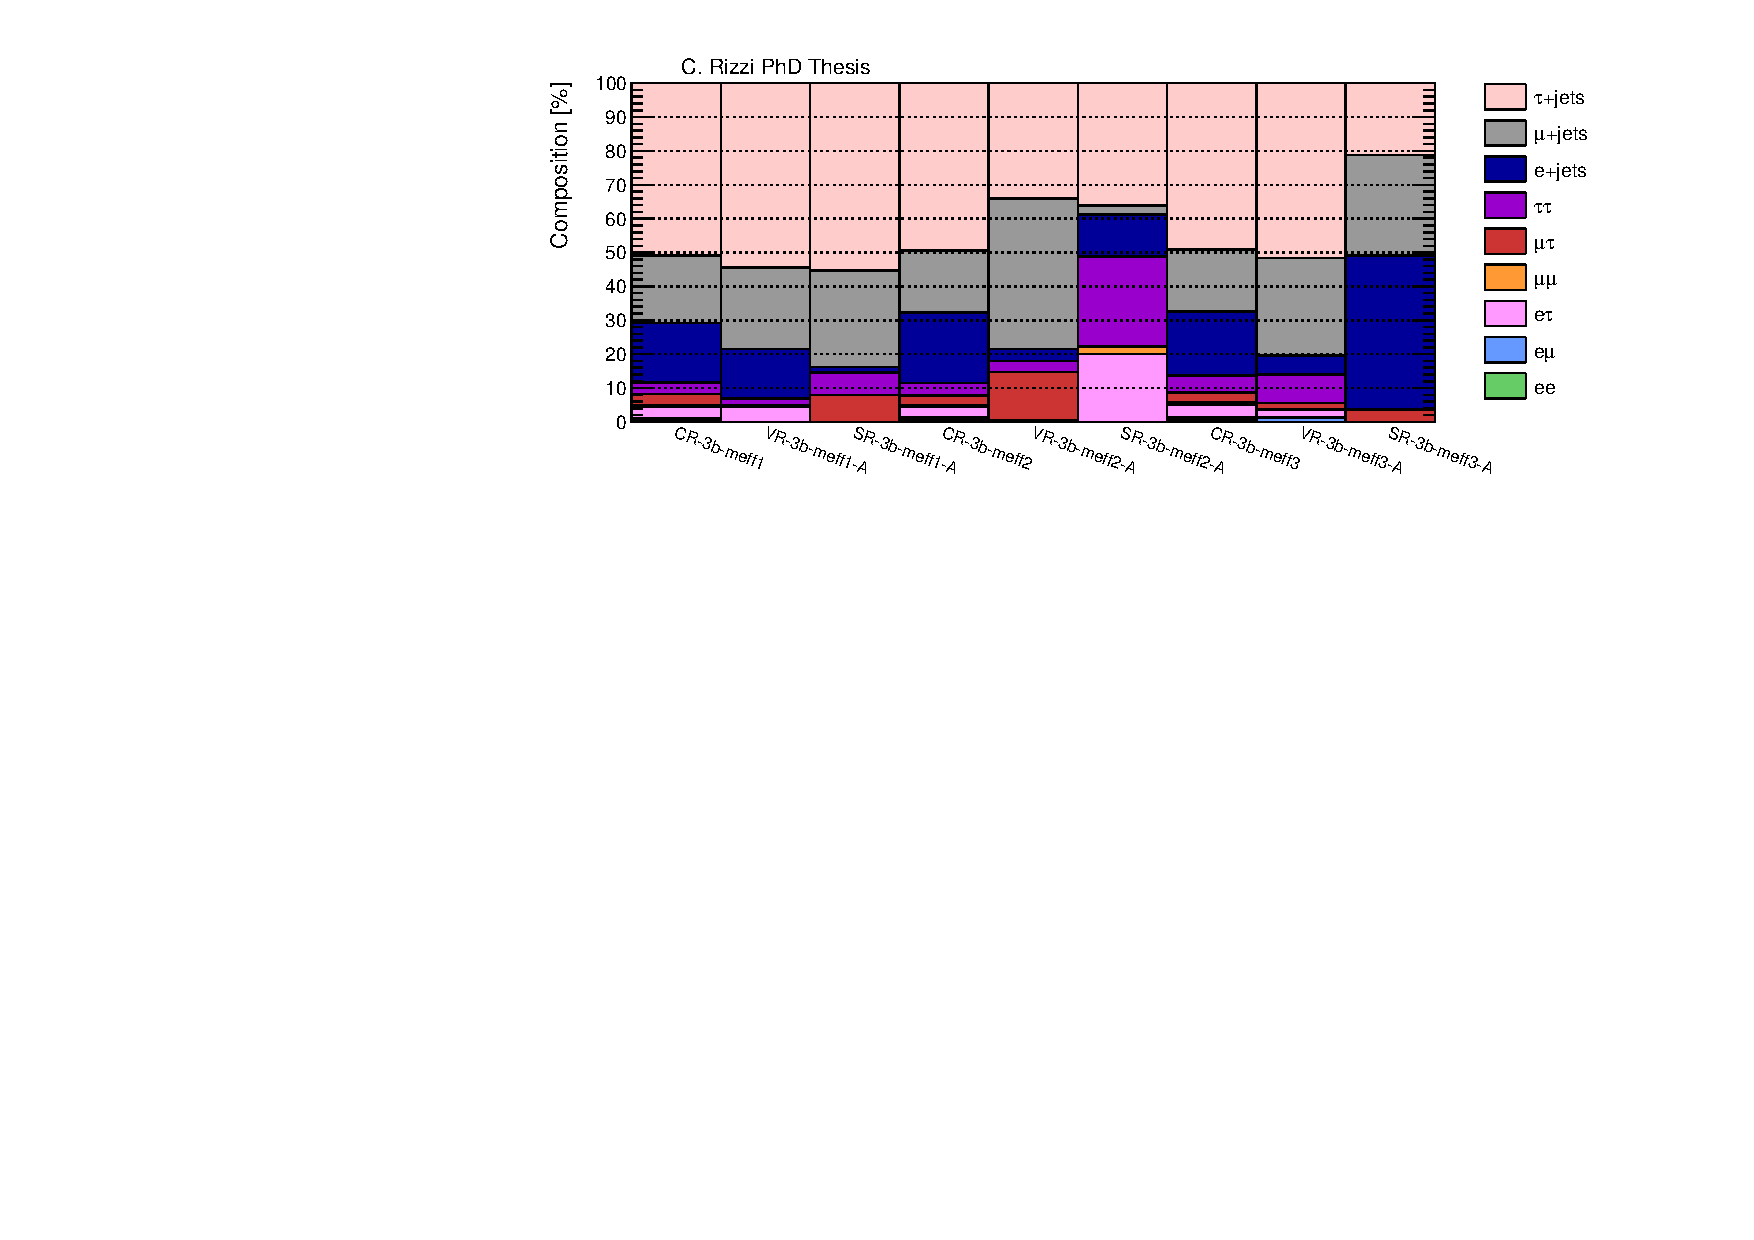
\includegraphics[width=\textwidth]{figures/ewk_prod/comp_plots/hh_3b_tt.pdf}
\caption{Decay mode of the \ttbar background in the regions with exactly three $b$-jets.}
	\label{fig:ttcomp_hh3b}
\end{figure}

\begin{figure}[htbp]
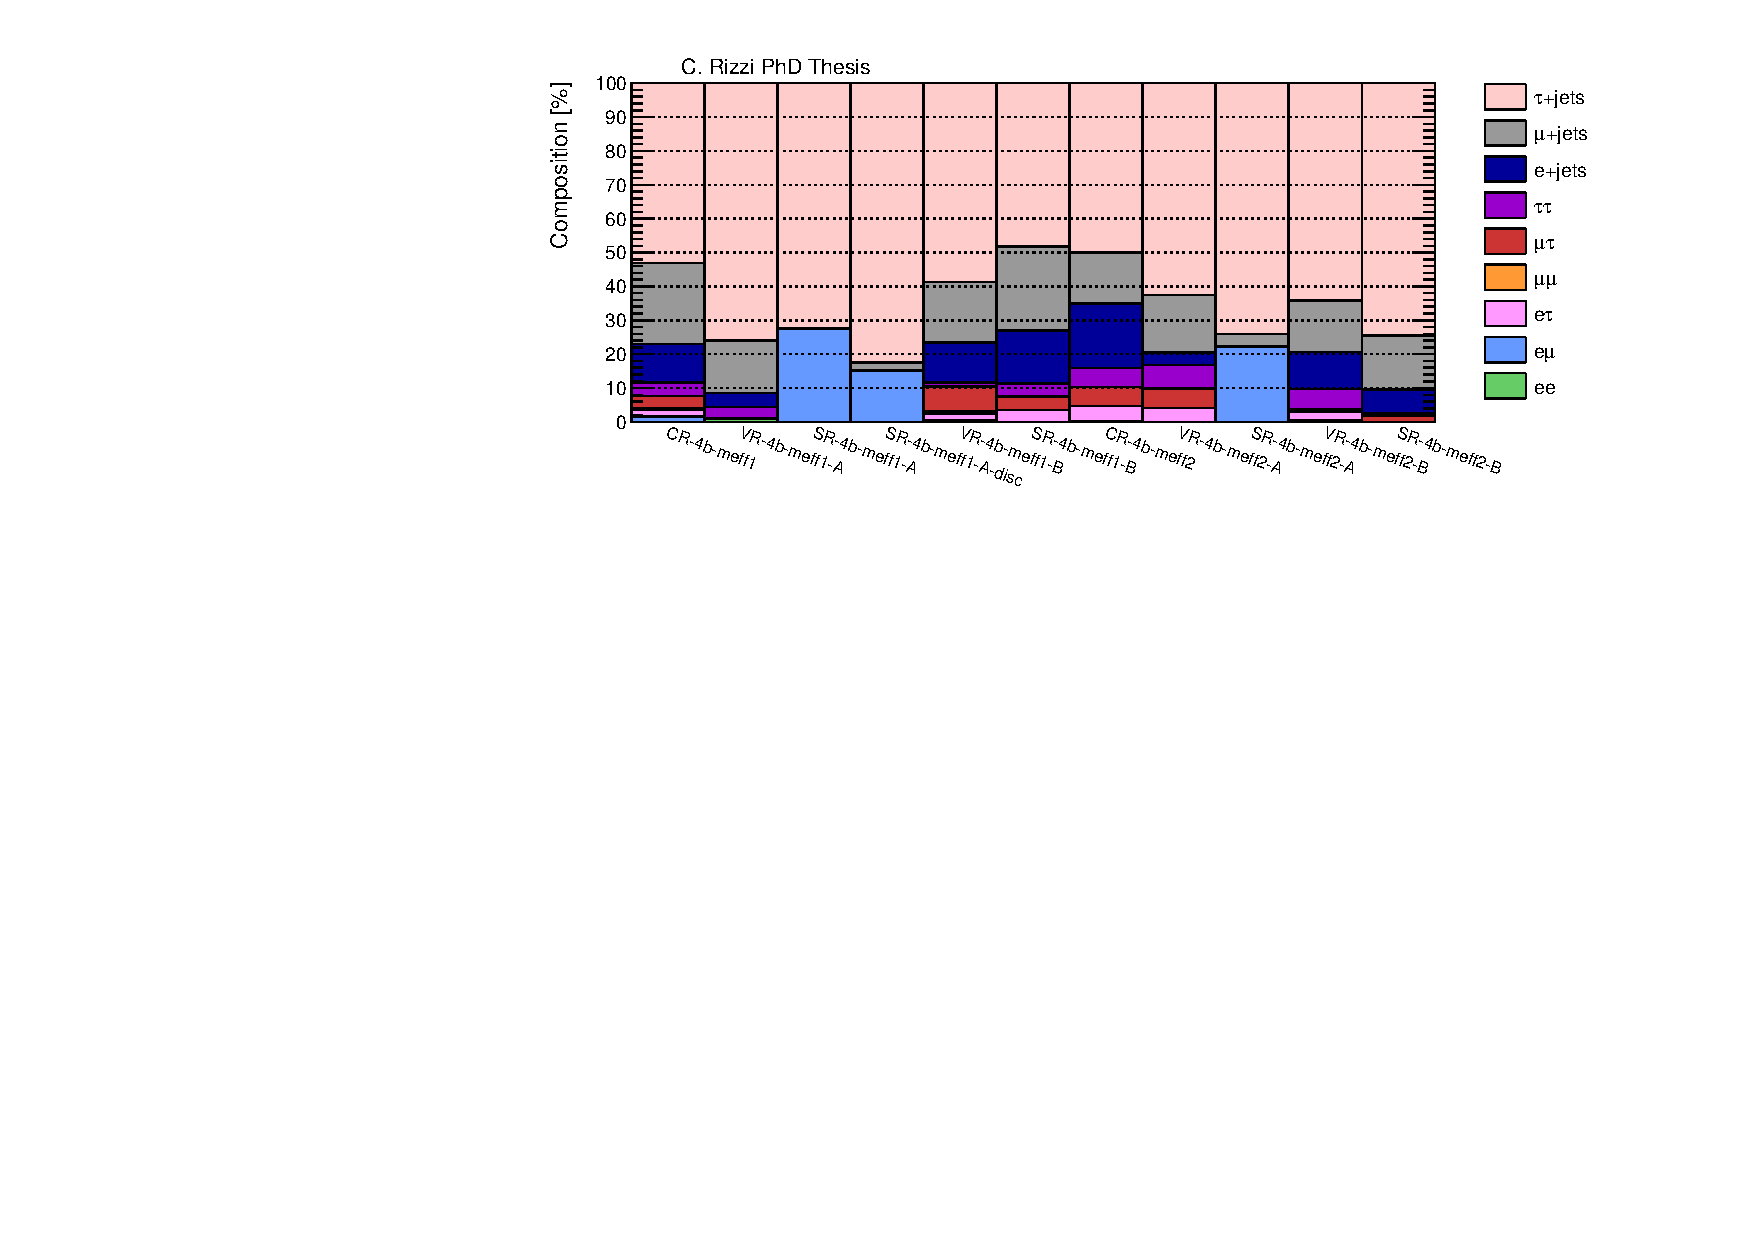
\includegraphics[width=\textwidth]{figures/ewk_prod/comp_plots/hh_4b_tt.pdf}
\caption{Decay mode of the \ttbar background in the regions with at least four $b$-jets.}
	\label{fig:ttcomp_hh4b}
\end{figure}

\begin{figure}[htbp]
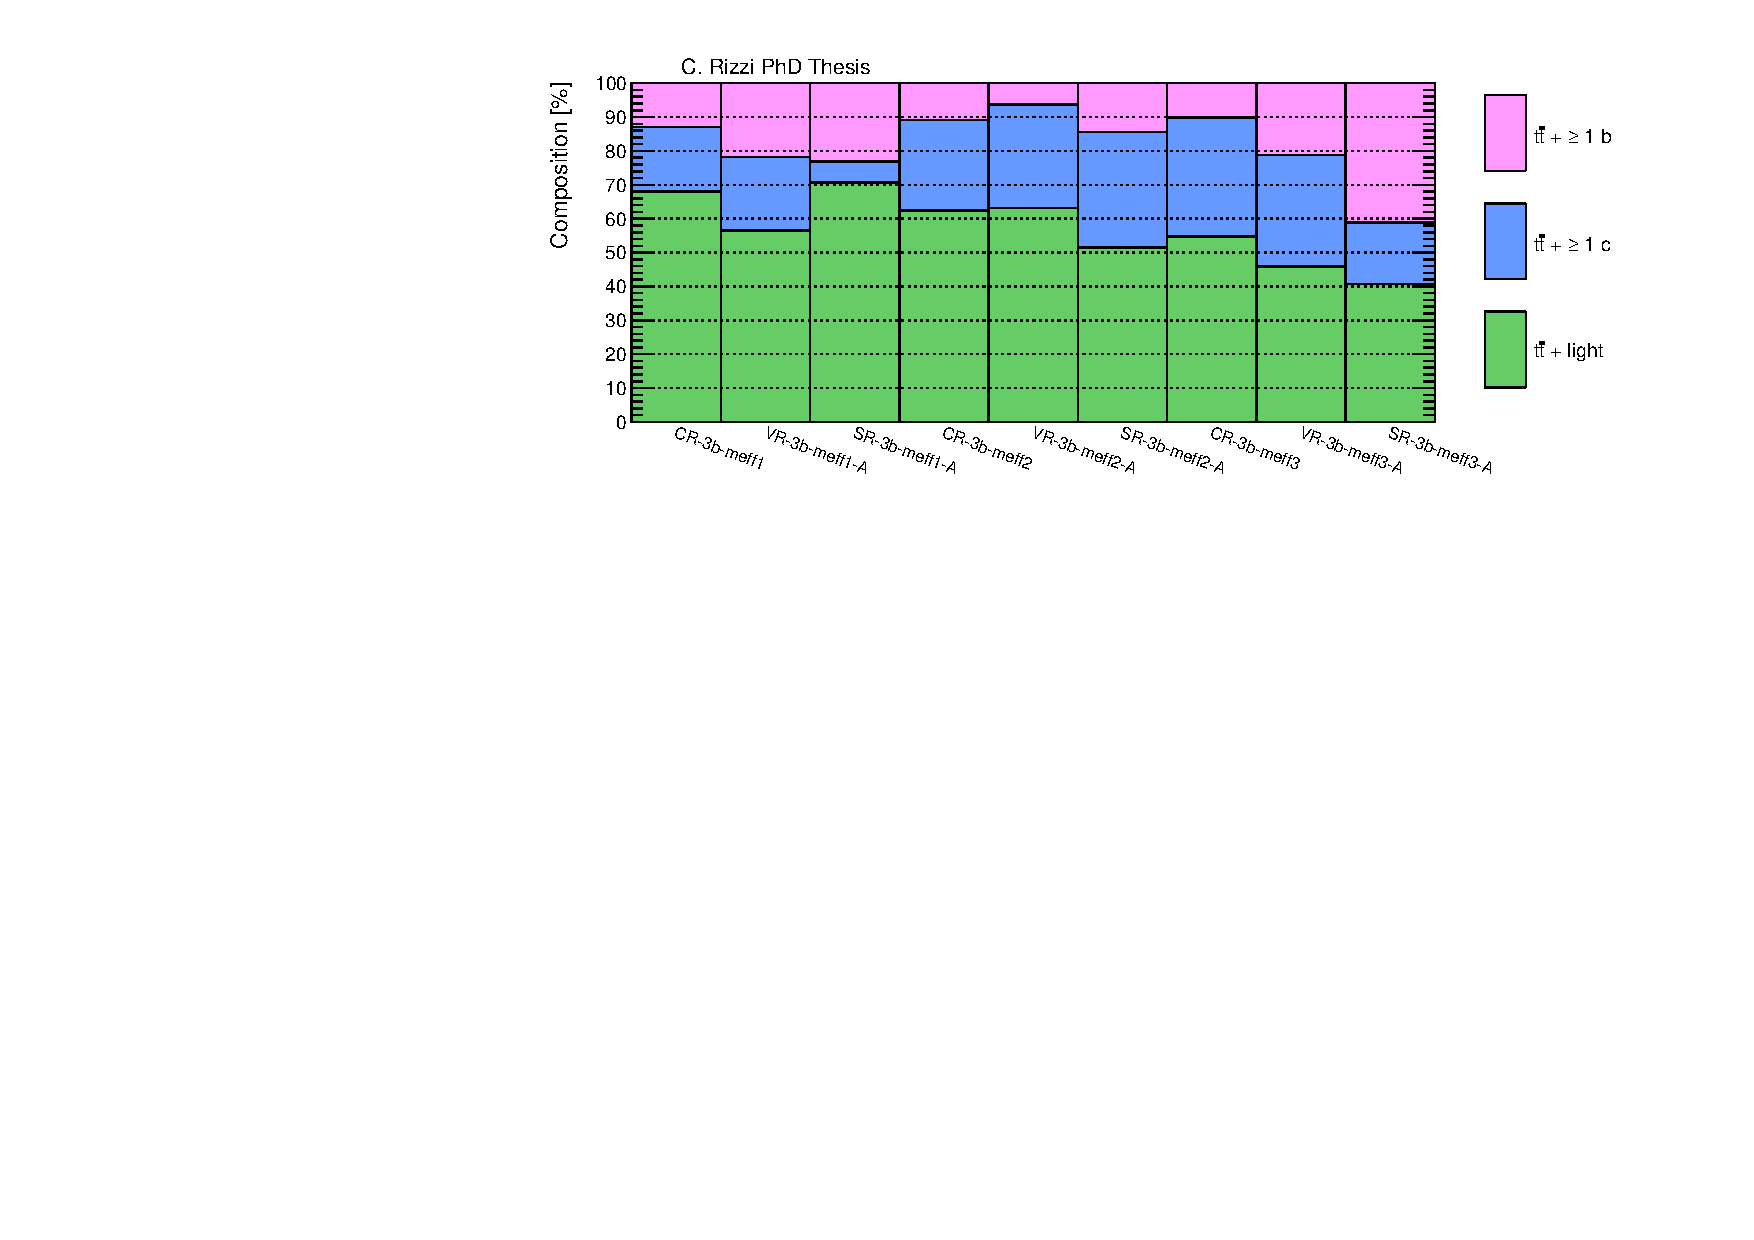
\includegraphics[width=\textwidth]{figures/ewk_prod/comp_plots/hh_3b_HF.pdf}
\caption{Heavy-flavor composition of the \ttbar background in regions with exactly three $b$-jets.}
	\label{fig:HFcomp_hh3b}
\end{figure}

\begin{figure}[htbp]
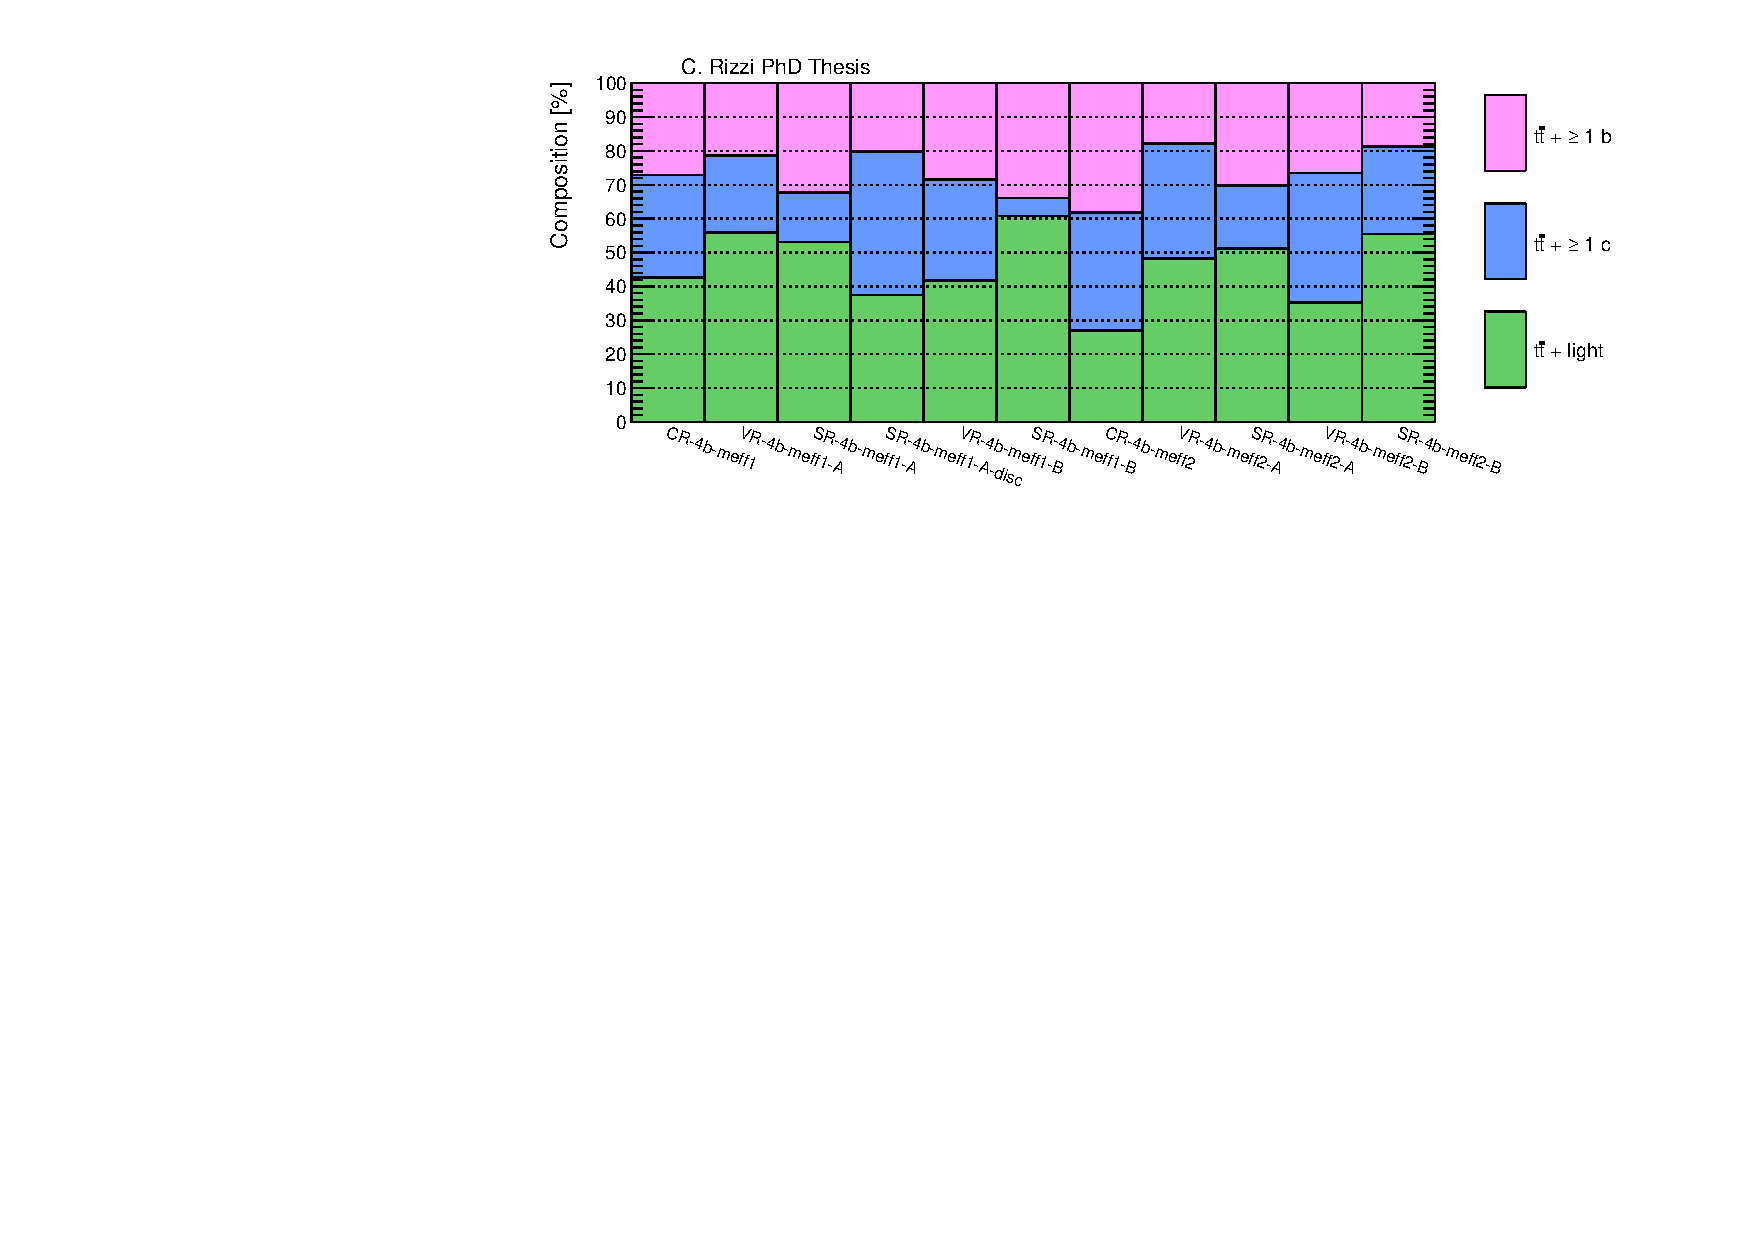
\includegraphics[width=\textwidth]{figures/ewk_prod/comp_plots/hh_4b_HF.pdf}
\caption{Heavy-flavor composition of the \ttbar background in regions with at least four $b$-jets.}
	\label{fig:HFcomp_hh4b}
\end{figure}

\FloatBarrier

\section{Comparison between data and simulation}
\label{sec:ewk:dataMC}

The modeling of the main kinematic variables is very similar to what observed in Section \ref{sec:strong:dataMC} 
for the strong-production multi-b analysis, as the few differences in object definitions are not enough to 
lead to a substantial change in the agreement between data and simulation; 
this section therefore focuses on the variables specific to Higgs boson reconstruction.
The comparison between data and simulation for the variables already shown in Section \ref{sec:strong:dataMC} but with the object definitions 
specific to this analysis are shown in Appendix \ref{app:ewk:datamc}.
There is nevertheless a notable exception: in the analysis described in this chapter, the agreement between data and simulation in the 
distribution of the number of $b$-jets is improved, as can be appreciated comparing Figure \ref{fig:strong:datamc0L:bjets_n} with Figure \ref{fig:ewk:datamc_bjets}.
This is the result of the improvement in the $b$-tagging calibration: as discussed in Section \ref{sec:obj:btaggingcalib}, 
the calibration of $c$-jets used in this analysis is based on \ttbar events, rather than on $W+c$ events as in the gluino analysis.
The other important difference with respect to the strong-production analysis is that in this case the analysis is performed 
only in regions with a lepton veto; it is not therefore sensitive to the mismodeling in the 1-lepton channel discussed in Section 
\ref{sec:strong:kinrw} and no kinematic reweighting is required. 

As shown in Figure \ref{fig:ewk:datamc_a}, all the variables specific to this analysis show a good 
agreement between data and the simulation. 

\begin{figure*}[htbp]
\centering 
%\subfigure[\nbjet]{
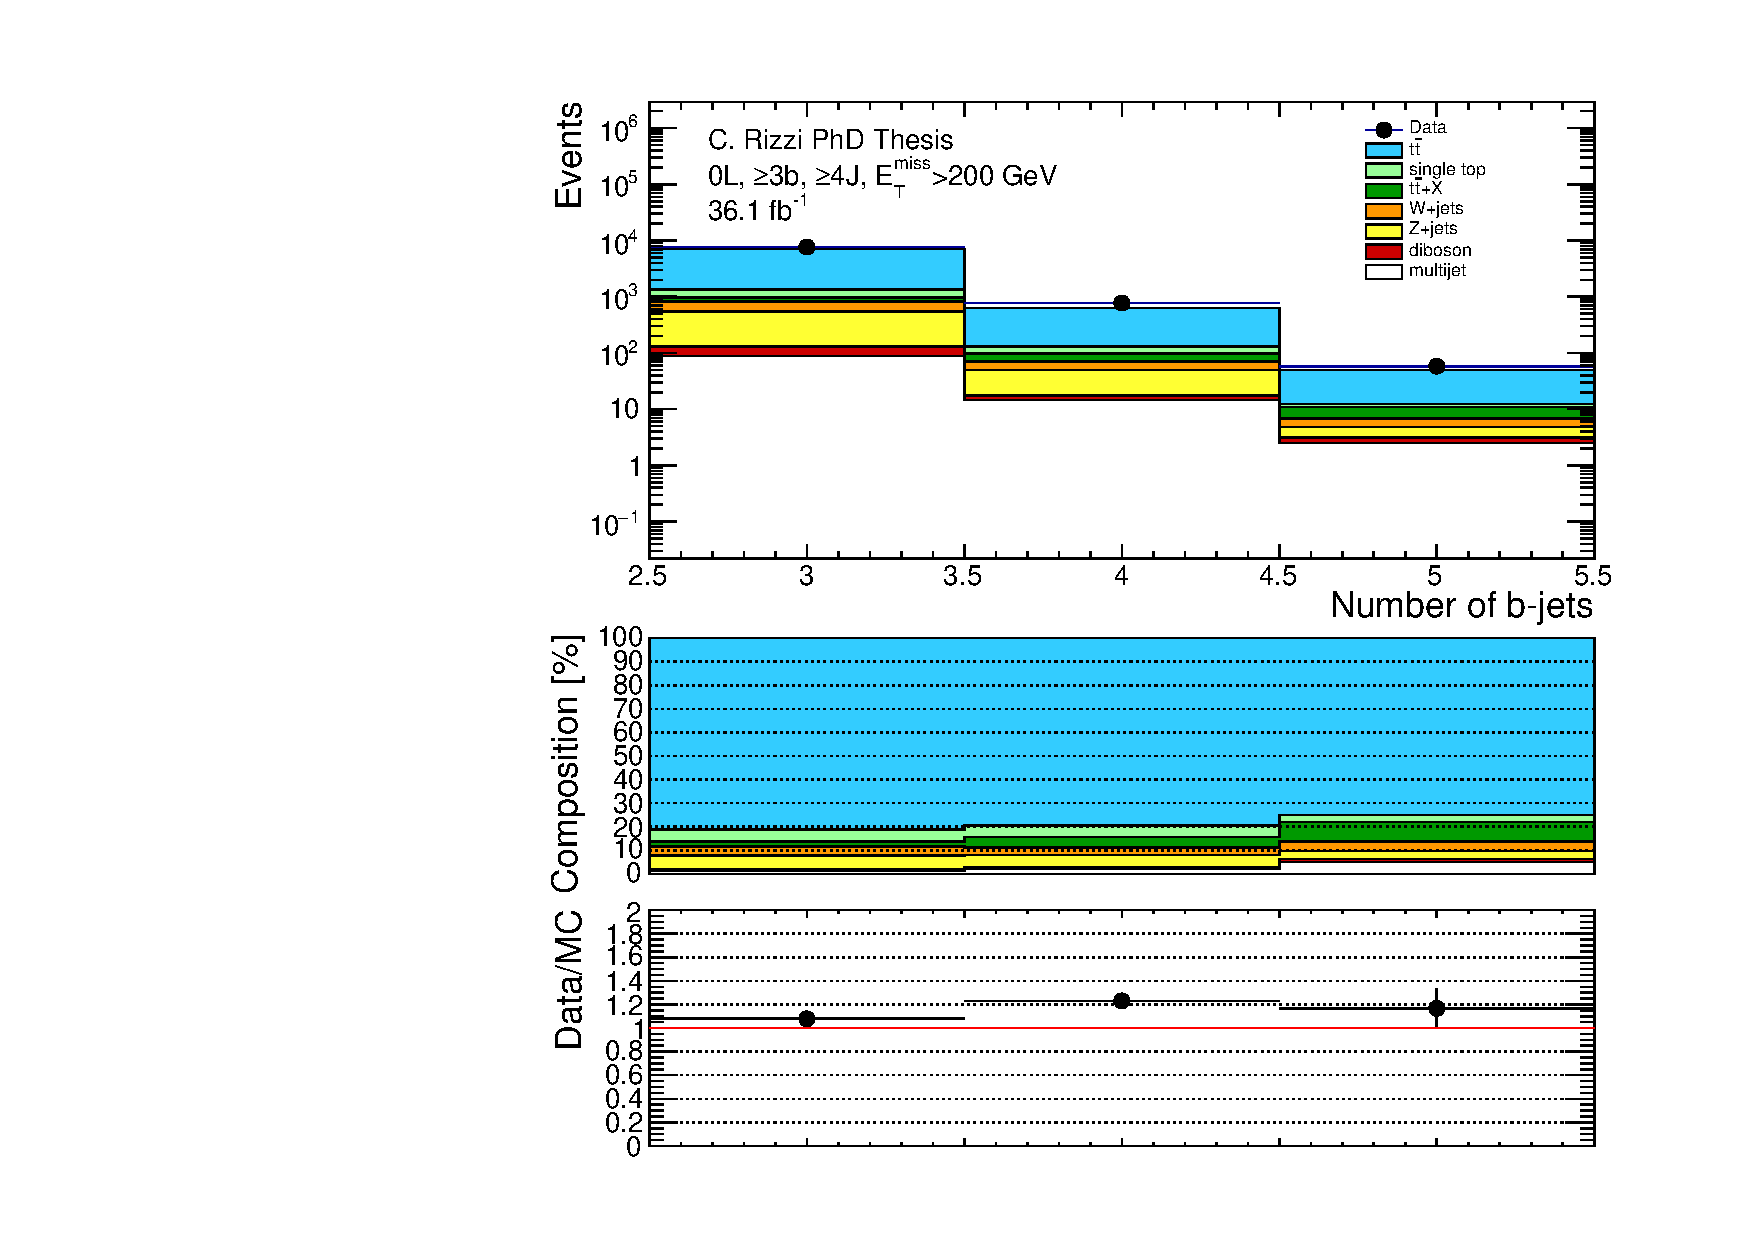
\includegraphics[width=0.45\textwidth]{figures/ewk_prod/data_mc/0L_3bin/data_mc_bjets_n.pdf}
%\label{fig:ewk:datamc:bjets_n}}\\
\caption{Comparison of the number of $b$-jets between data and simulation in the preselection described in the text.
}
\label{fig:ewk:datamc_bjets}
\end{figure*}

\begin{figure*}[htbp]
\centering 
\subfigure[m($h_1$)]{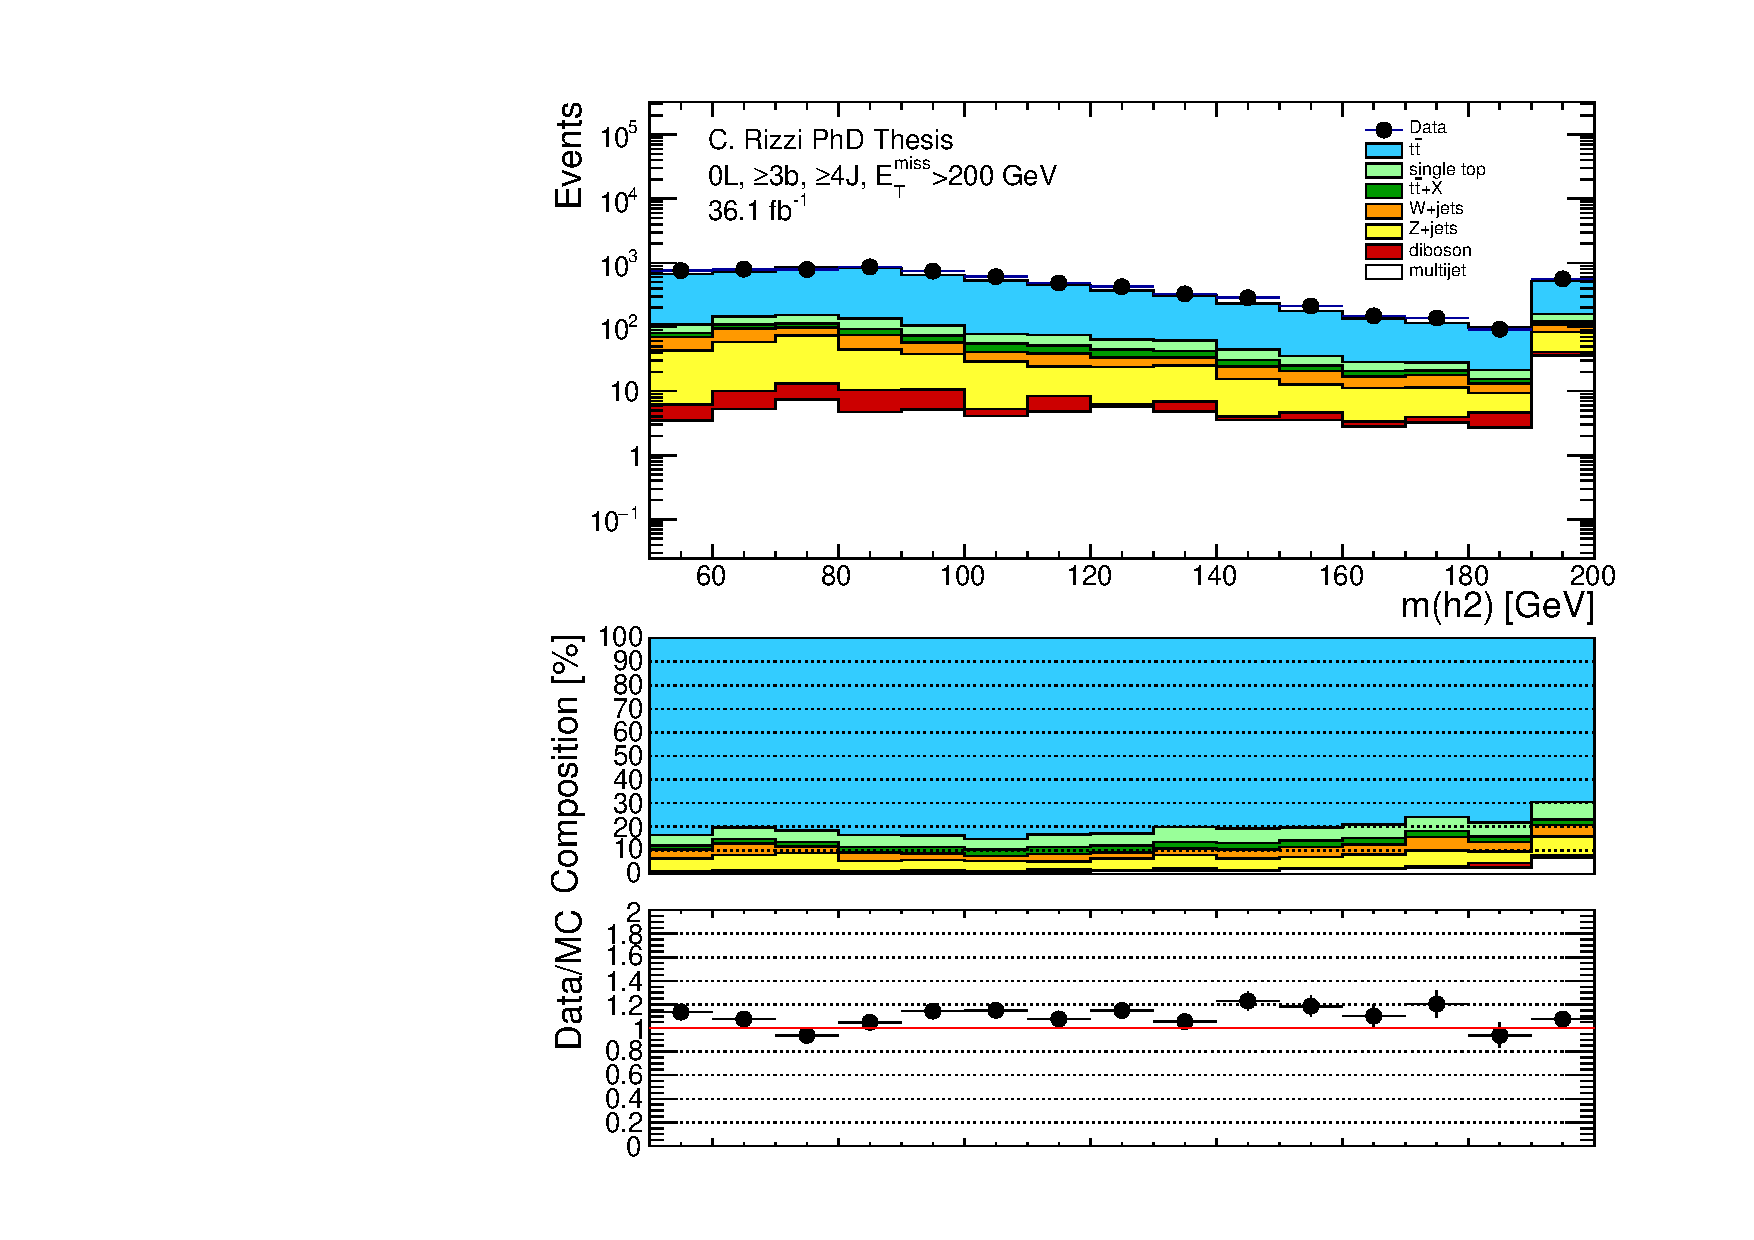
\includegraphics[width=0.45\textwidth]{figures/ewk_prod/data_mc/0L_3bin/data_mc_mass_h2_min_dR.pdf}
\label{fig:ewk:datamc:mass_h2_min_dR}}
\subfigure[m($h_2$)]{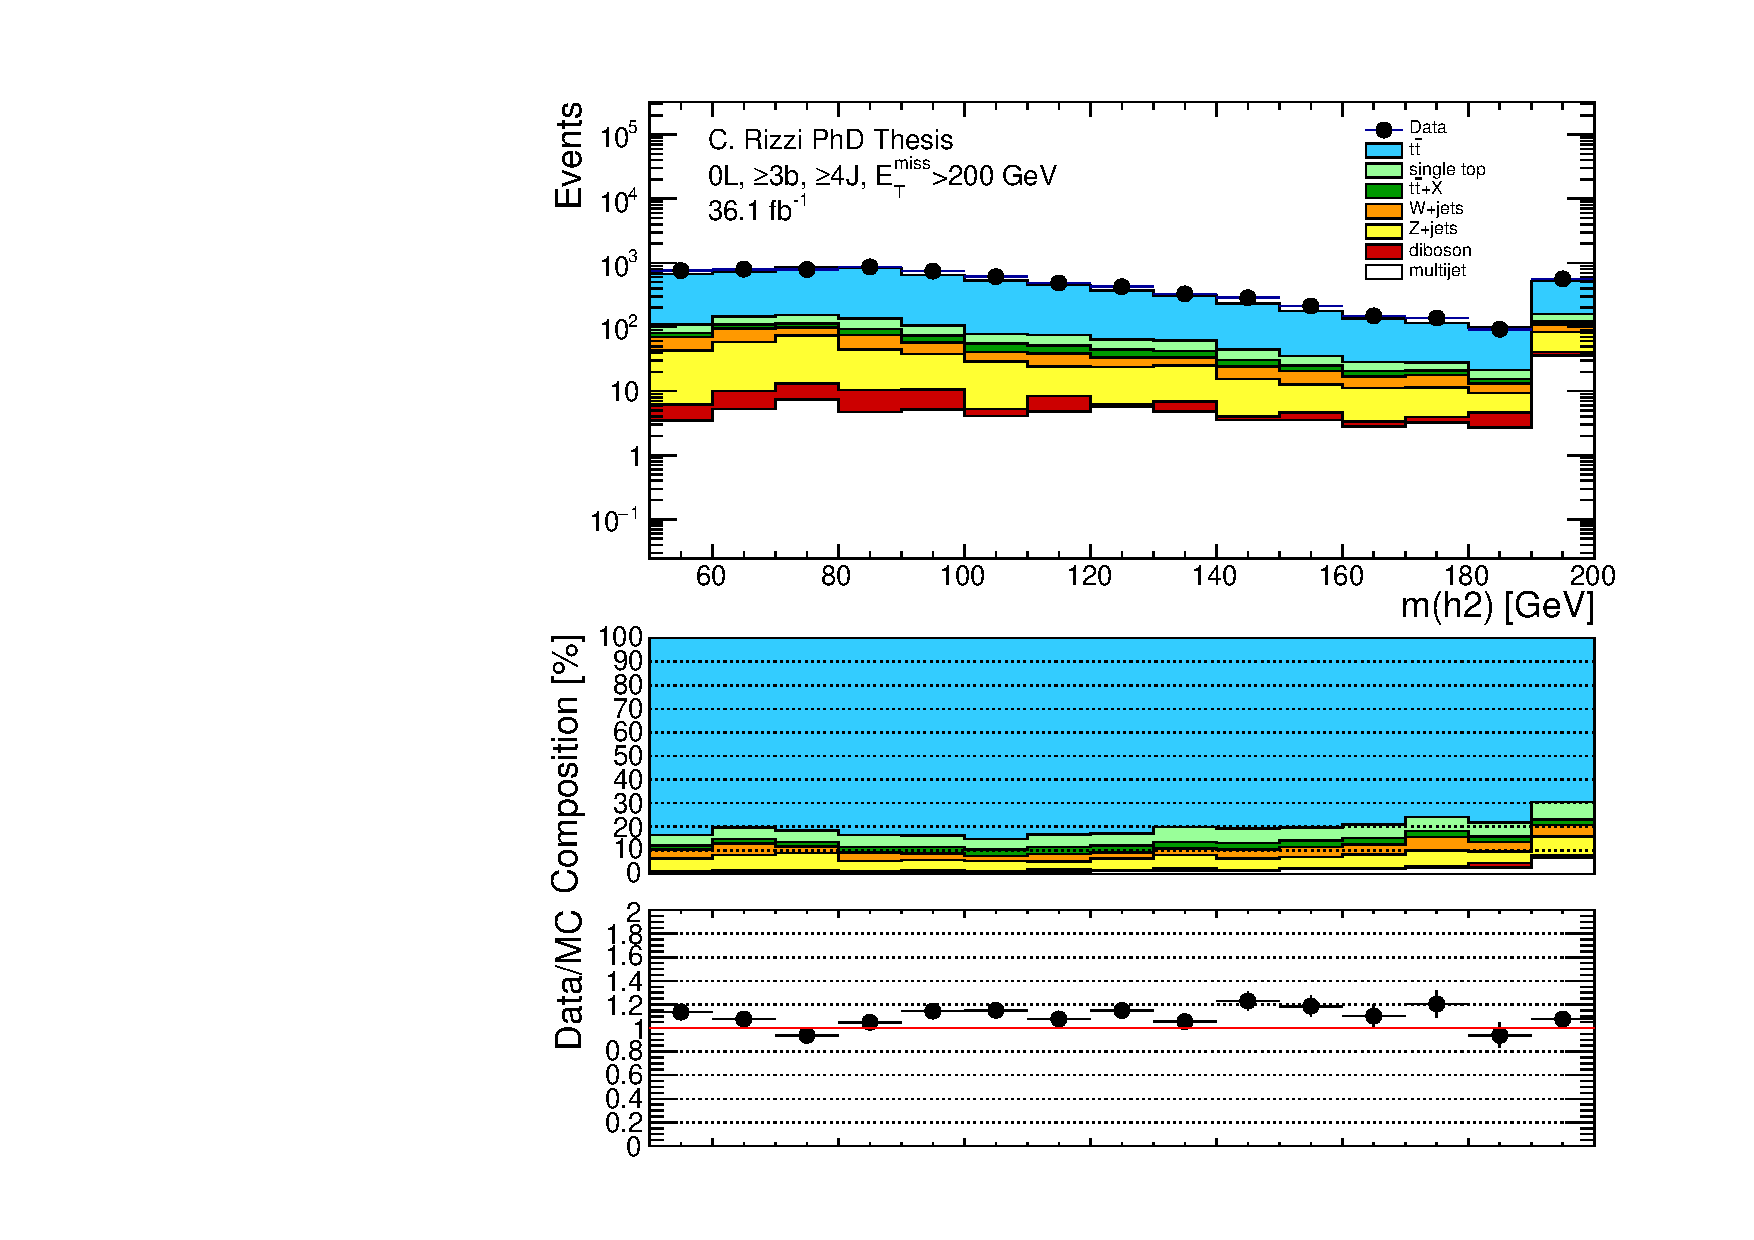
\includegraphics[width=0.45\textwidth]{figures/ewk_prod/data_mc/0L_3bin/data_mc_mass_h2_min_dR.pdf}
\label{fig:ewk:datamc:mass_h2_min_dR}}\\
\subfigure[\dRmax]{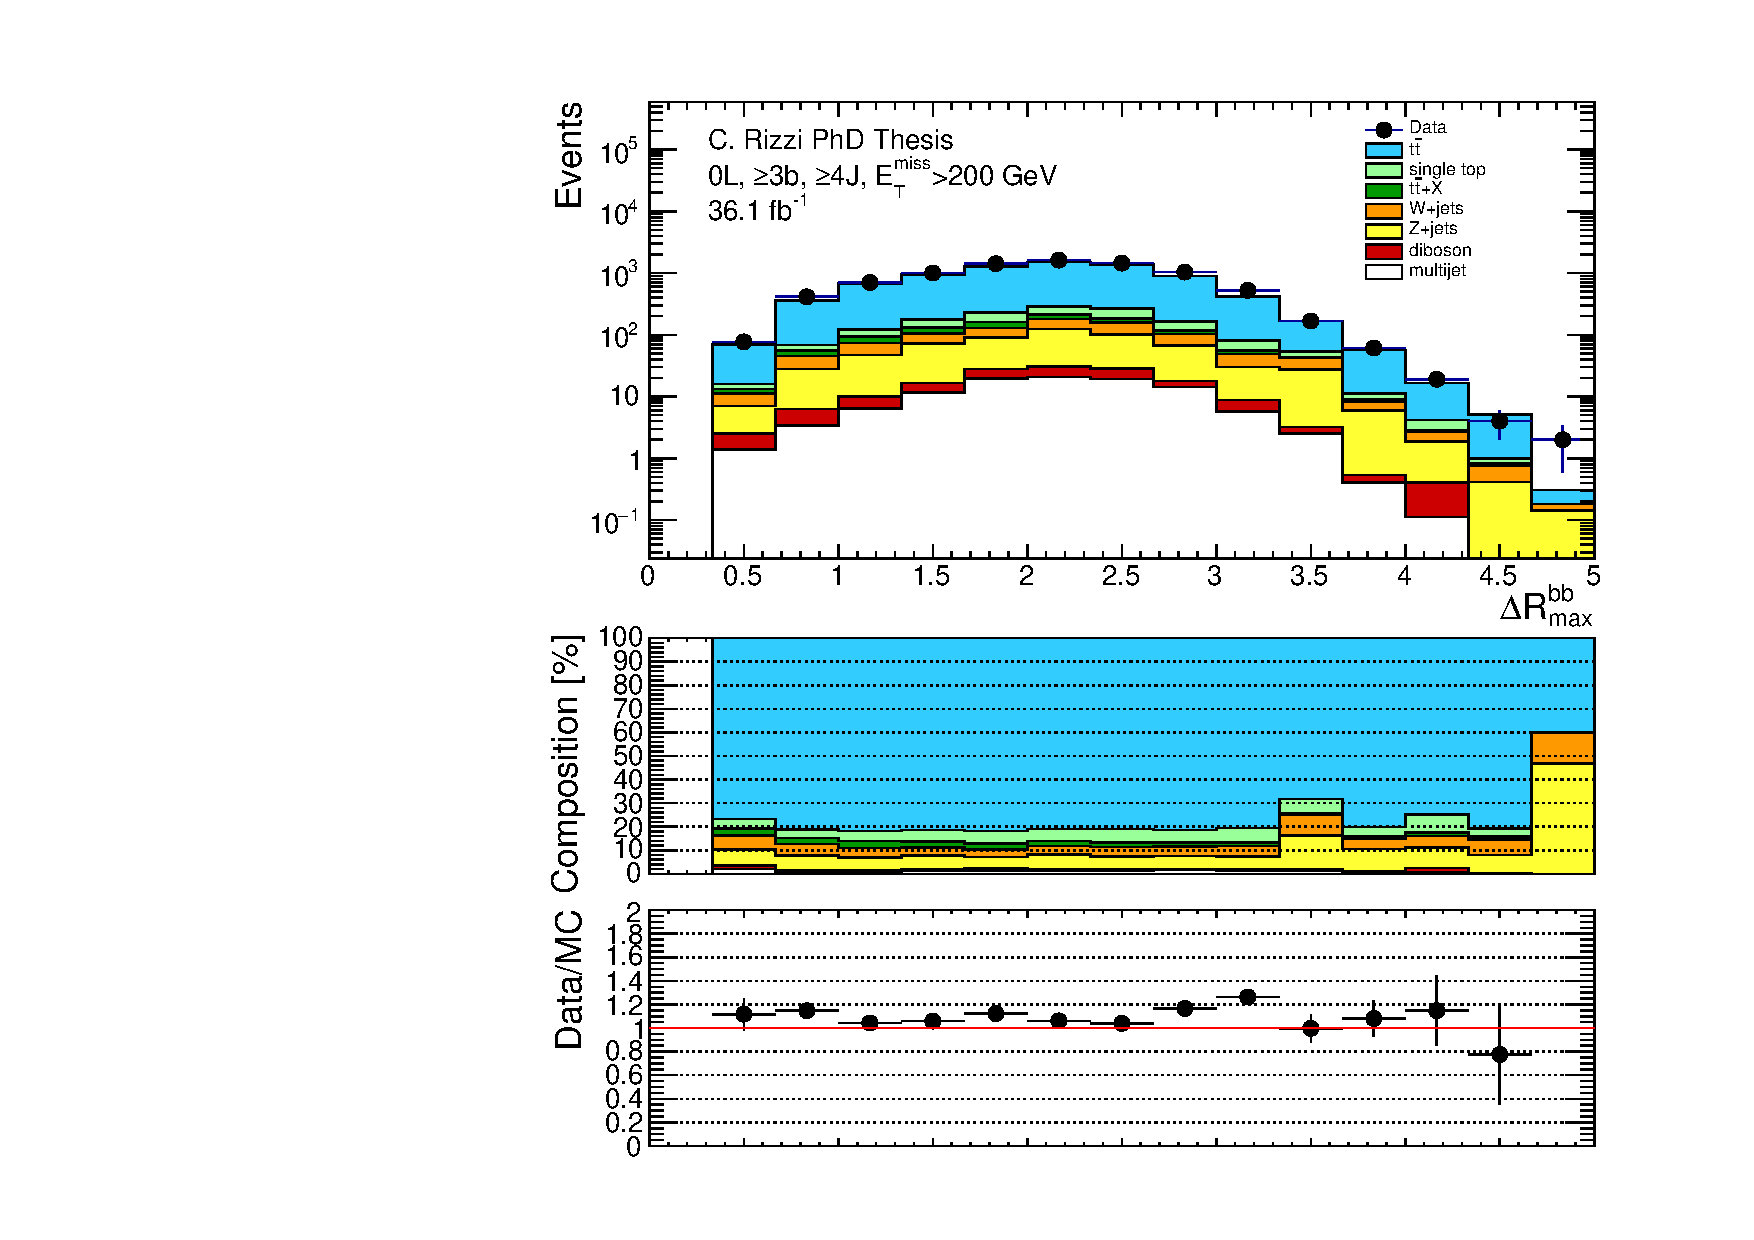
\includegraphics[width=0.45\textwidth]{figures/ewk_prod/data_mc/0L_3bin/data_mc_dRmax_dR.pdf}
\label{fig:ewk:datamc:dRmax_dR}}
\subfigure[\meffb]{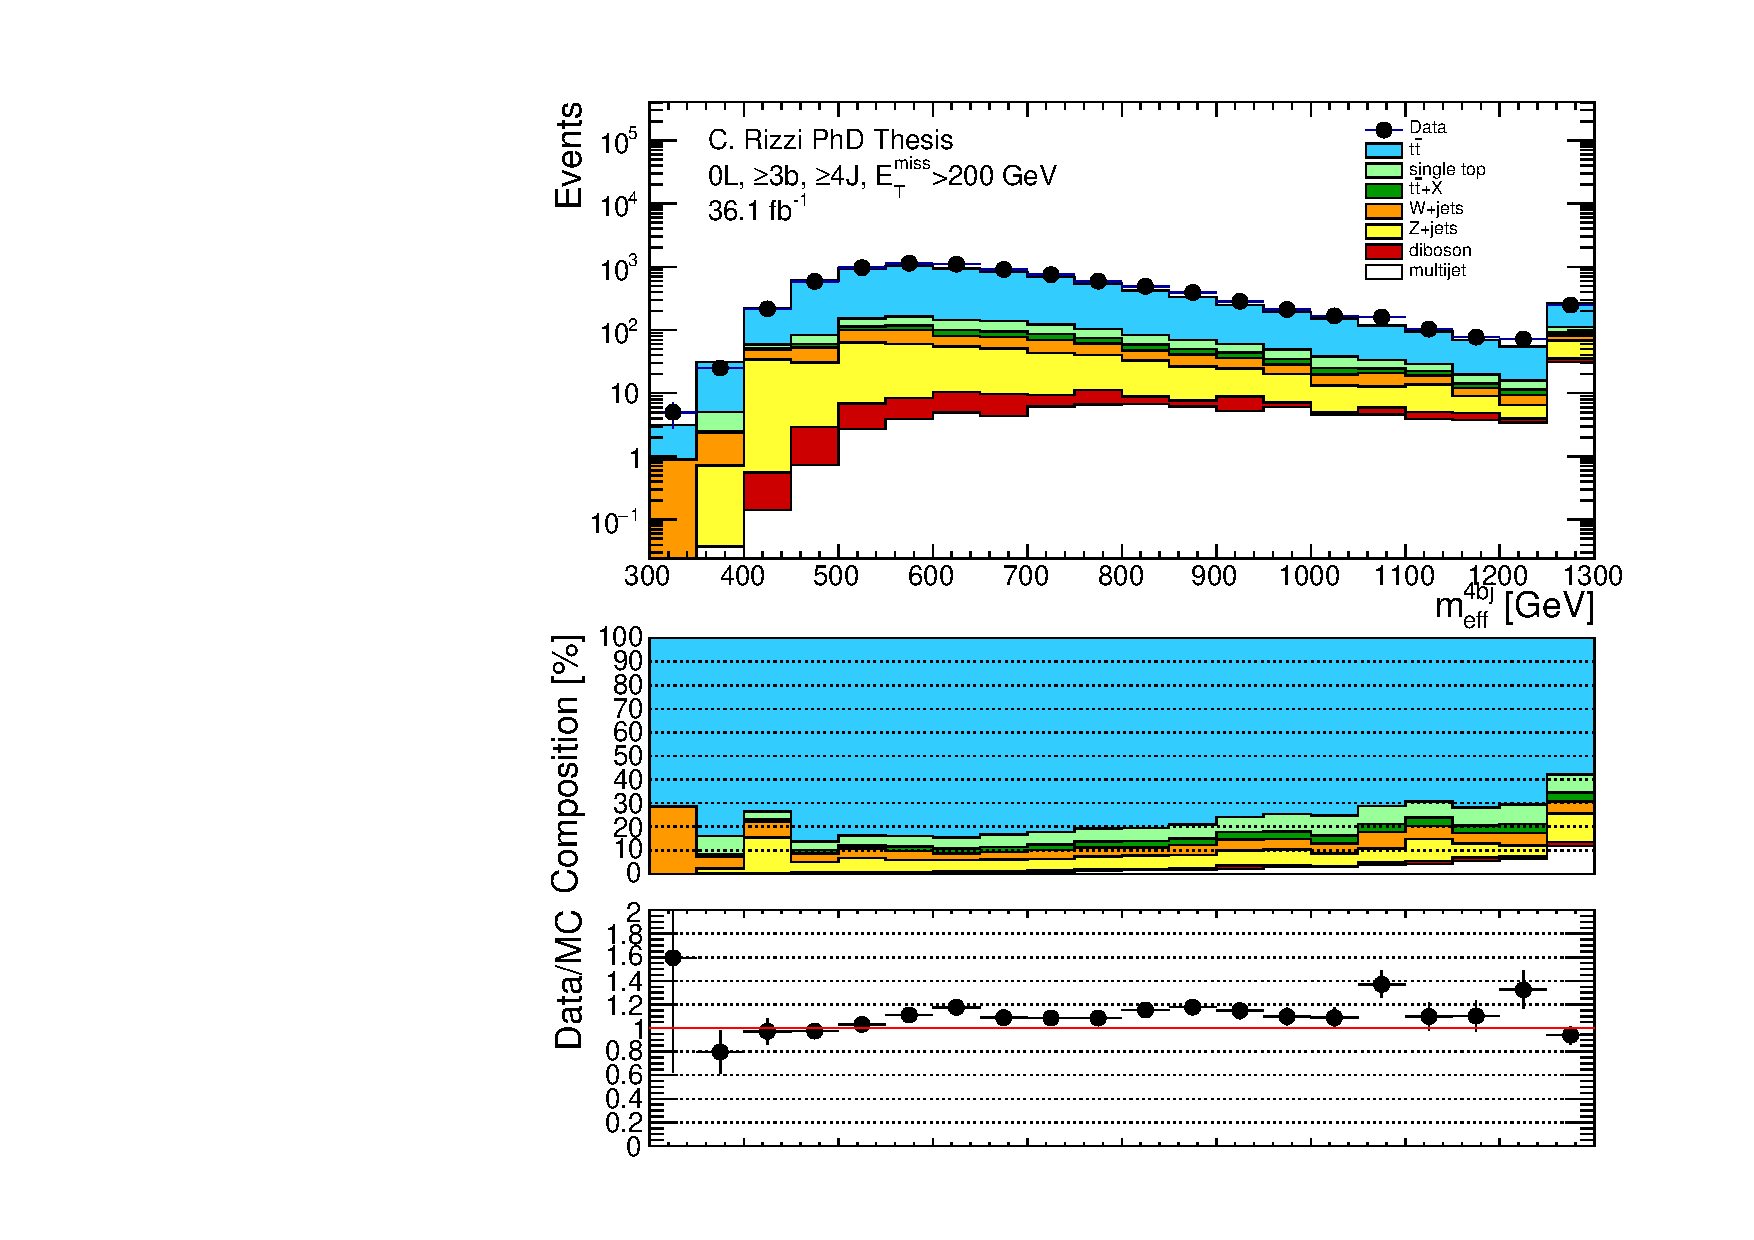
\includegraphics[width=0.45\textwidth]{figures/ewk_prod/data_mc/0L_3bin/data_mc_meff_4bj.pdf}
\label{fig:ewk:datamc:pt_meff_4bj}}
\caption{Comparison between data and simulation in the preselection described in the text.
}
\label{fig:ewk:datamc_a}
\end{figure*}

\clearpage

